\section{Отбор эталонов}
Как правило, работа с выборками большого объёма сопряжена с большими затратами времени на обучение модели. Кроме этого, в достаточно популярном методе \(k\) ближайших соседей обучающая выборка хранится полностью, что в случае выборки большого объёма является ограничивающим для него фактором. Таким образом, привлекательными кажутся техники, которые позволяют уменьшить объём обучающей выборки, почти не теряя обобщающей способности. Данная тематика в литературе на английском языке называется instance selection (prototype selection).

В \cite{ps-taxonomy} было проведено крупномасштабное исследование, а также классификация методов отбора объектов обучающей выборки. Авторы разбили их на следующие группы по механизму работы:
\begin{itemize}
    \item методы сгущения (condensation) --- стремятся сократить число точек, далёких от границ классов, в предположении, что они слабо влияют на геометрию границы. Они стремятся сохранить качество классификации на обучающей выборке, при этом качество классификации на тестовой выборке может пострадать. Тем не менее, они, как правило, достигают высокой степени сокращения объёма обучающей выборки;
    \item методы редактирования (edition) --- стремятся сократить число точек, близких к границам классов, несогласованных с соседними, шумовых точек. Данные методы создают более гладкие границы между классами, и приводят к повышению обобщающей способности классификатора, но они в меньшей степени сокращают объём выборки, чем методы предыдущей группы;
    \item гибридные методы (hybrid) --- стремятся найти подмножество выборки как можно меньшей мощности, которое улучшает обобщающую способность на тестовых данных.
\end{itemize}

Столкнувшись со значительными затратами вычислительных ресурсов при тестировании различных методов машинного обучения в нашей задаче, мы решили опробовать несколько методов отбора эталонов и оценить, насколько большую пользу они могут принести в данной задаче. В пакете scikit-learn данный класс методов не представлен, а существующие реализации на Python \cite{scikit-protopy} показали себя неудовлетворительно с точки зрения производительности. Поэтому для проведения данной работы методы condensed nearest neighbor (CNN), fast condensed nearest neigbor (FCNN) и class conditional instance selection (CCIS), реализованные авторами \cite{ps-taxonomy}, были портированы на язык C. В следующих подразделах выбранные методы отбора эталонов описаны и приведены результаты, показанные ими на нашей задаче.

Все представленные в данном разделе методы используют \(k\)NN для внутренних нужд: оценки подмножеств обучающей выборки, нахождения новых элементов для добавления в неё или удаления из неё. Значительное количество методов, исследованных в \cite{ps-taxonomy} опираются на \(k\)NN (в частности, из-за того, что они чаще всего применяются в связке с \(k\)NN классификатором). Тем не менее, спектр методов отбора эталонов ими не ограничивается, часть методов в \cite{ps-taxonomy} относится к классу эволюционных. Некоторые из них могут агрессивно редуцировать обучающую выборку и обеспечивать хорошое качество классификации. К сожалению, данные методы требуют значительно больших затрат времени, чем рассматриваемые далее, что не позволило нам оценить их в рамках данной работы.

\subsection{Condensed nearest neighbor}
Данный метод хронологически является одним из первых методов отбора эталонов. Он был описан в 1966 году в \cite{hart} вместе с понятием \emph{согласованного подмножества} (consistent subset) обучающей выборки \(T\) --- такого подмножества \(S\subseteq T\), что метод ближайшего соседа, обученный на \(S\), правильно классифицирует \(T\setminus S\). Он представляет из себя простейший метод сгущения и оперирует с двумя множествами: \(S\) и \(R\). Изначально \(S\) содержит лишь первый элемент обучающей выборки, а \(R=\varnothing\). Второй элемент классифицируется методом ближайшего соседа на основе множества \(S\), и, если ему присвоен верный класс, то он добавляется в \(R\), иначе он добавляется в \(S\). Каждый следующий элемент \(T\) обрабатывается аналогичным образом. После первого прохода через \(T\) процедура начинает совершать проходы через множество \(R\), до тех пор, пока за весь проход через \(R\) ни один элемент не будёт перенесён в \(S\), после чего в \(S\) находится согласованное подмножество \(T\).

Метод CNN был сформулирован для метода одного ближайшего соседа, однако расширение на \(k\) ближайших соседей производится очевидным образом: при классификации очередного элемента \(T\) (а впоследствии \(R\)) используется метод \(k\)NN с обучающей выборкой \(S\). Стоит отметить, что данный метод строит согласованное подмножество только по отношению к методу \(k\) ближайших соседей (для конкретного \(k\)), результирующее подмножество \(S\) не обязано быть согласованным для произвольного алгоритма классификации.

\subsubsection*{Результаты применения CNN}
Были проведены эксперименты с методом CNN для \(k\in\{1, 5, 10\}\). На рис.~\ref{fig:cnn-stats} указаны результаты, показанные непосредственно CNN: время работы и доля отобранных объектов. Оказалось, что в нашей задаче доля отобранных объектов не имеет ярко выраженной зависимости от \(k\). Время работы ожидаемо зависит от \(k\) линейно (в реализации был использован наивный алгоритм \(k\)NN с перебором всех соседей).

\begin{figure}[h!]
    \centering
	\begin{subfigure}{0.45\textwidth}
		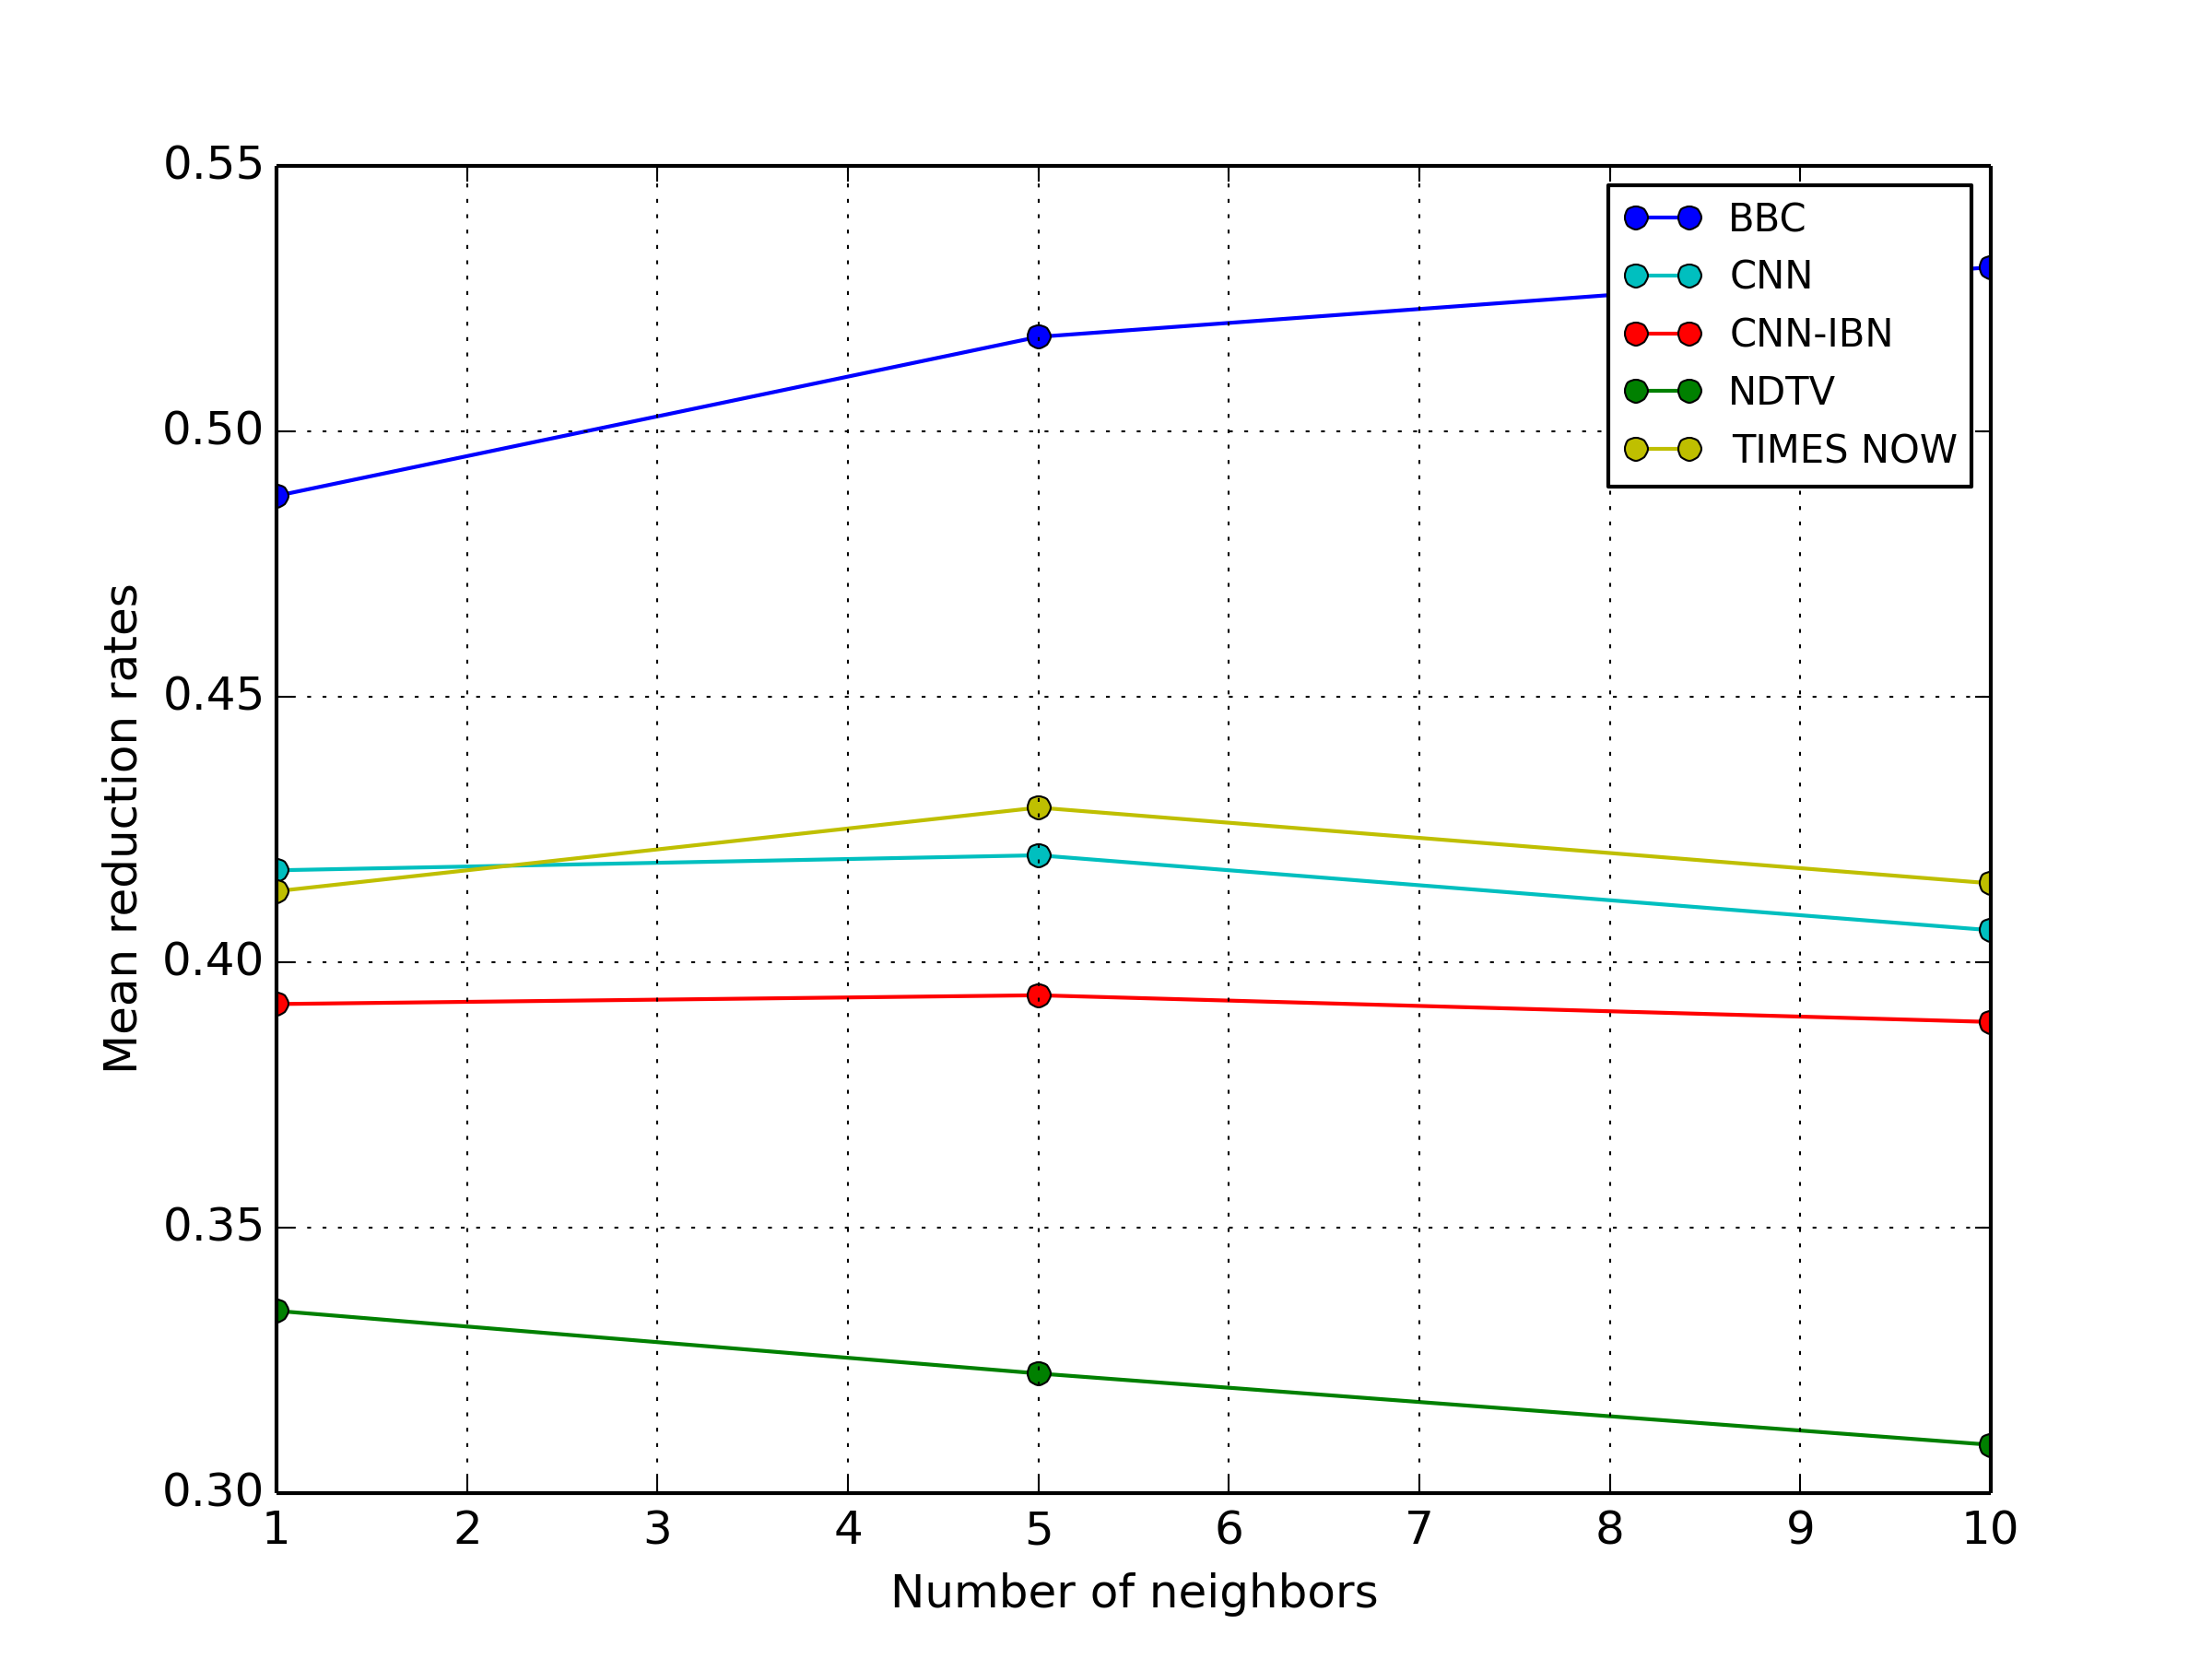
\includegraphics[width=\textwidth]{images/cnn-stats.png}
		\caption{Доля отобранных объектов.}
	\end{subfigure}
	\begin{subfigure}{0.45\textwidth}
		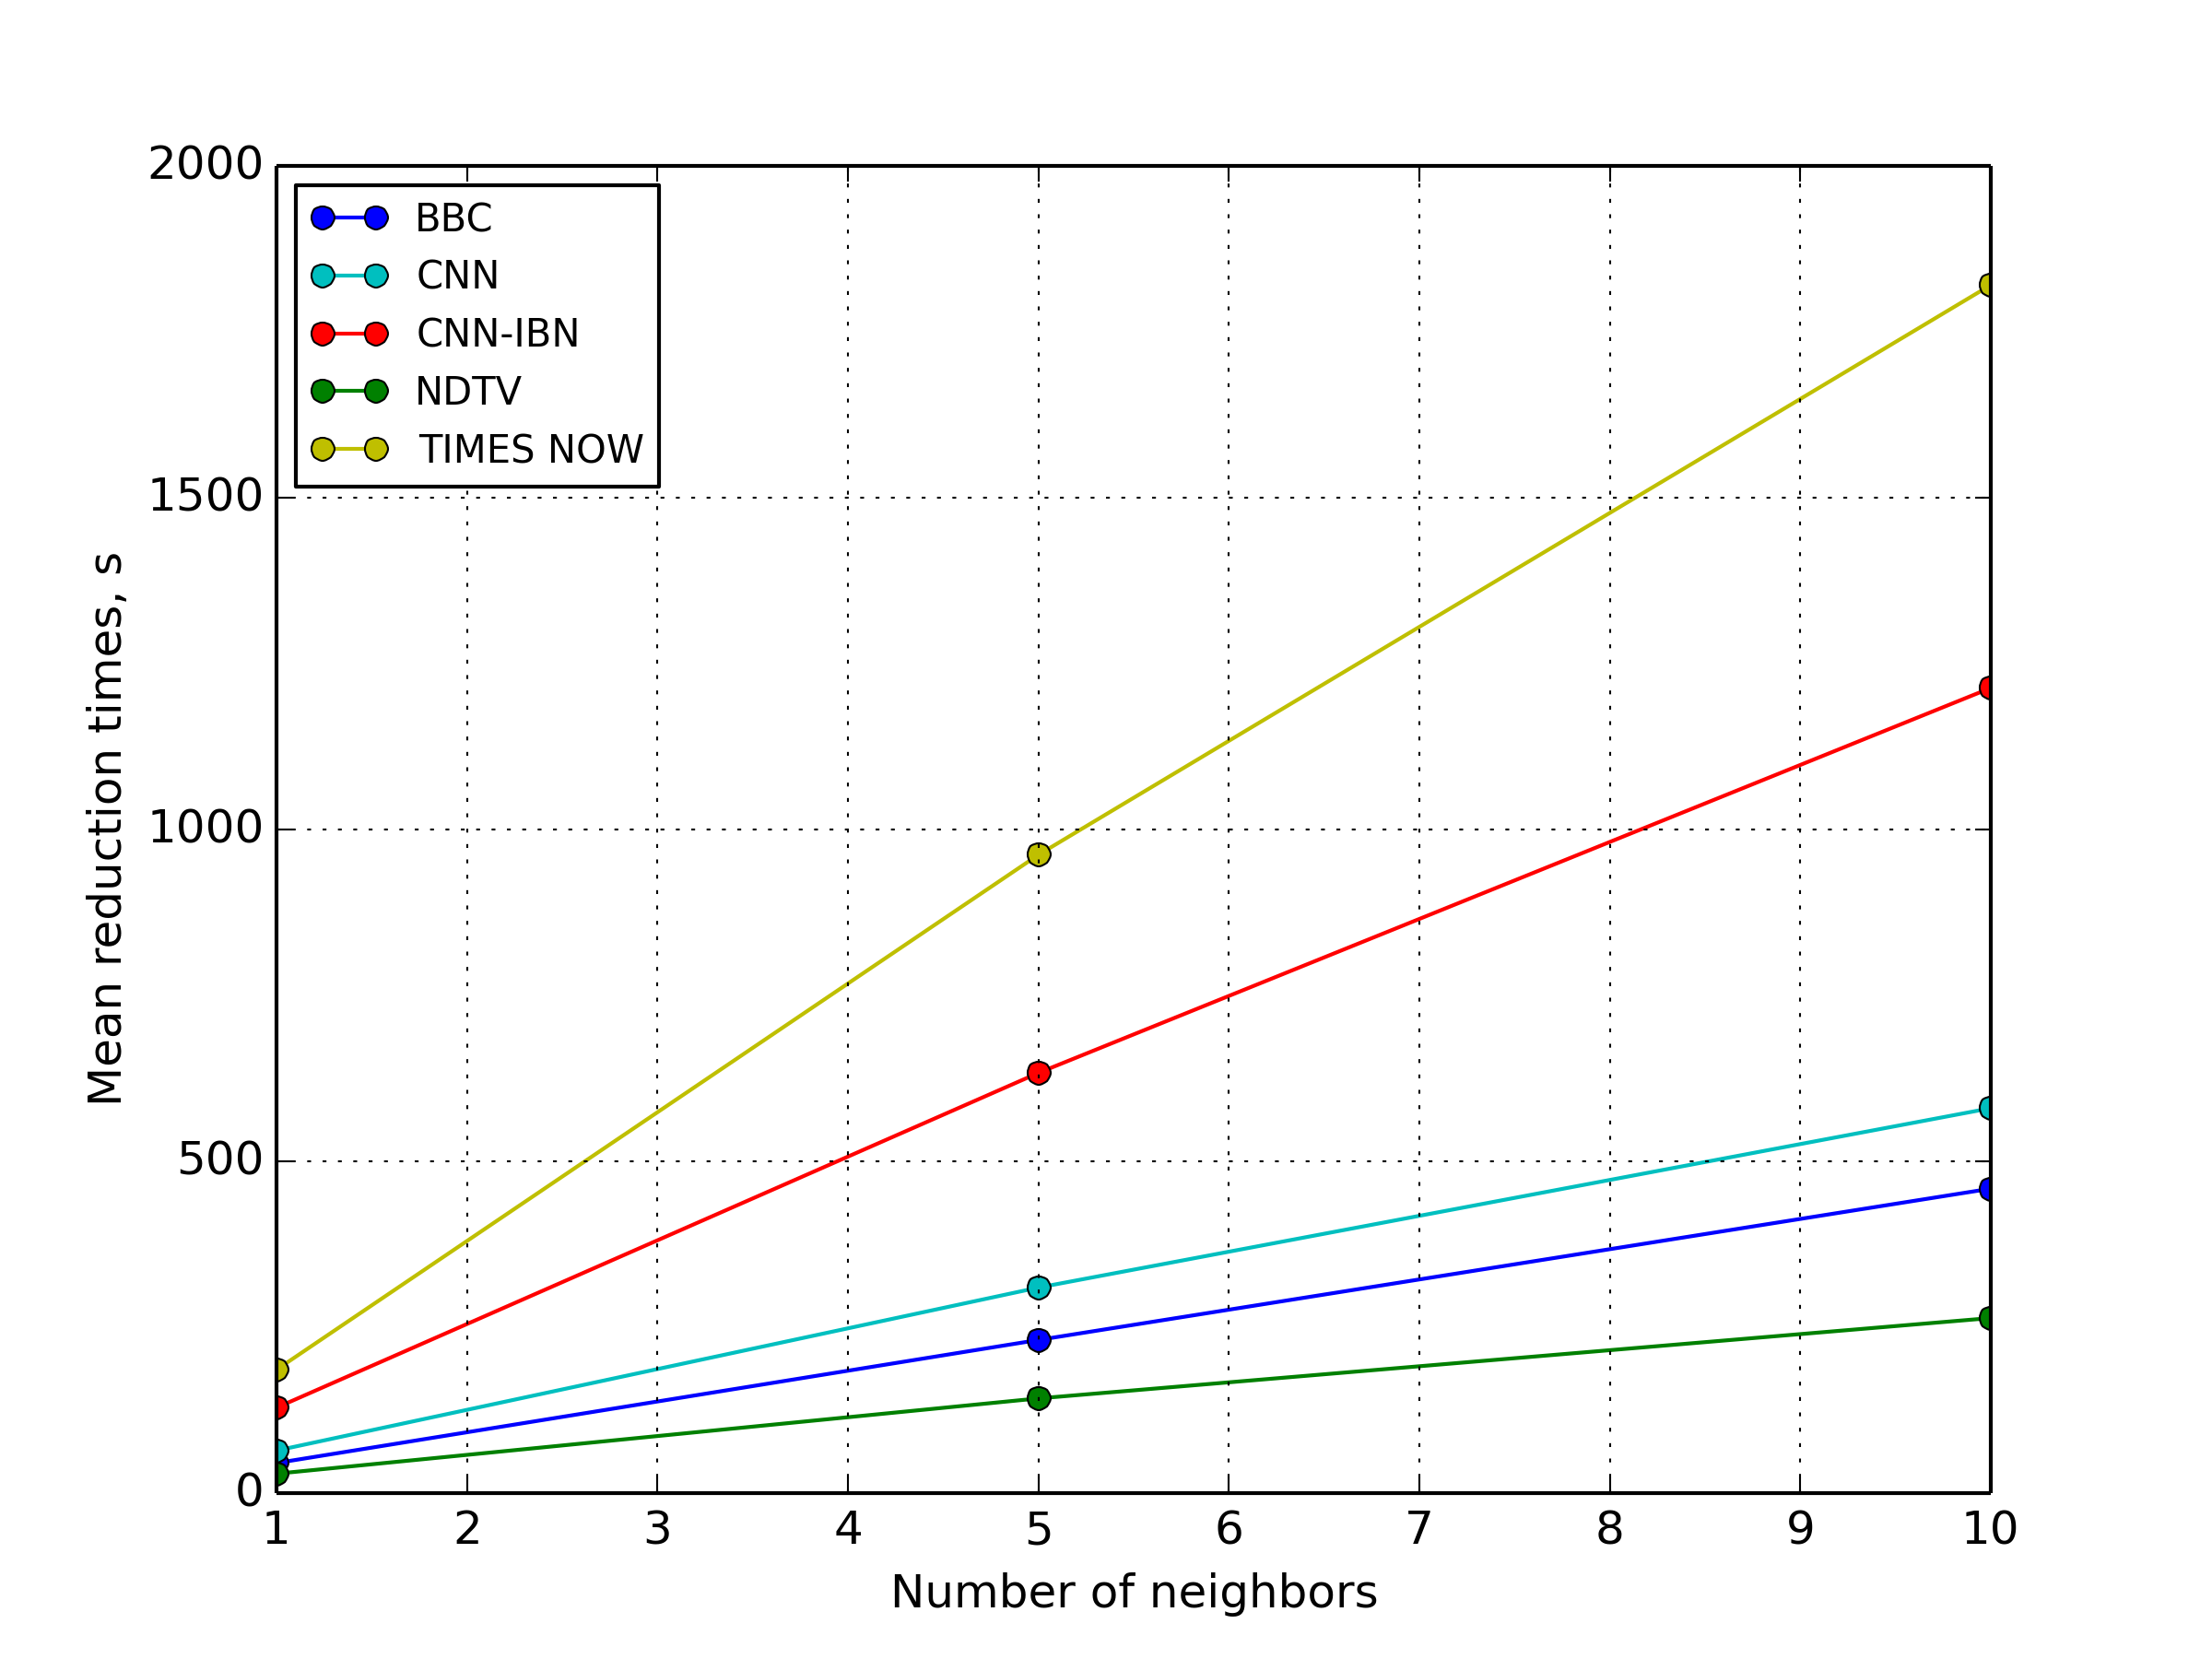
\includegraphics[width=\textwidth]{images/cnn-TimeStats.png}
		\caption{Время, потраченное на отбор эталонов.}
	\end{subfigure}
	\caption{Результаты работы CNN.}\label{fig:cnn-stats}
\end{figure}

На рис.~\ref{fig:cnn-knn-results}--\ref{fig:cnn-gtb-results} приведены результаты работы базовых методов на обучающих выборках, редуцированных с помощью CNN. При использовании \(k\), отличных от 1, CNN выбирает примерно такое же количество эталонов, как и при \(k=1\), но сами эталоны оказываются хуже по качеству. Этот результат не выглядит неожиданным, если учесть, что CNN, будучи методом сгущения, стремится оставить объекты, близкие к границе классов --- объекты, у которых много соседей из другого класса. За исключением каналов TIMES NOW и CNN-IBN для метода SVM использование \(k>1\) также не приносит ускорения базового метода классификации, в основном, потому что \(\left|S\right|\) получается примерно такой же. Иными словами, в данной задаче нет смысла использовать CNN с \(k>1\).

Тот факт, что CNN строит согласованное подмножество для \(k\)NN, наводит на вопрос: насколько хороший результат покажет 15-NN на выходе CNN с \(k=15\)? Такой эксперимент был проведён с одним каналом NDTV и он привёл к неудовлетворительным результатам: качество классификации оказалось близким к случаю \(k=10\) (около 25\%).

\begin{figure}[h!]
    \centering
	\begin{subfigure}{0.45\textwidth}
		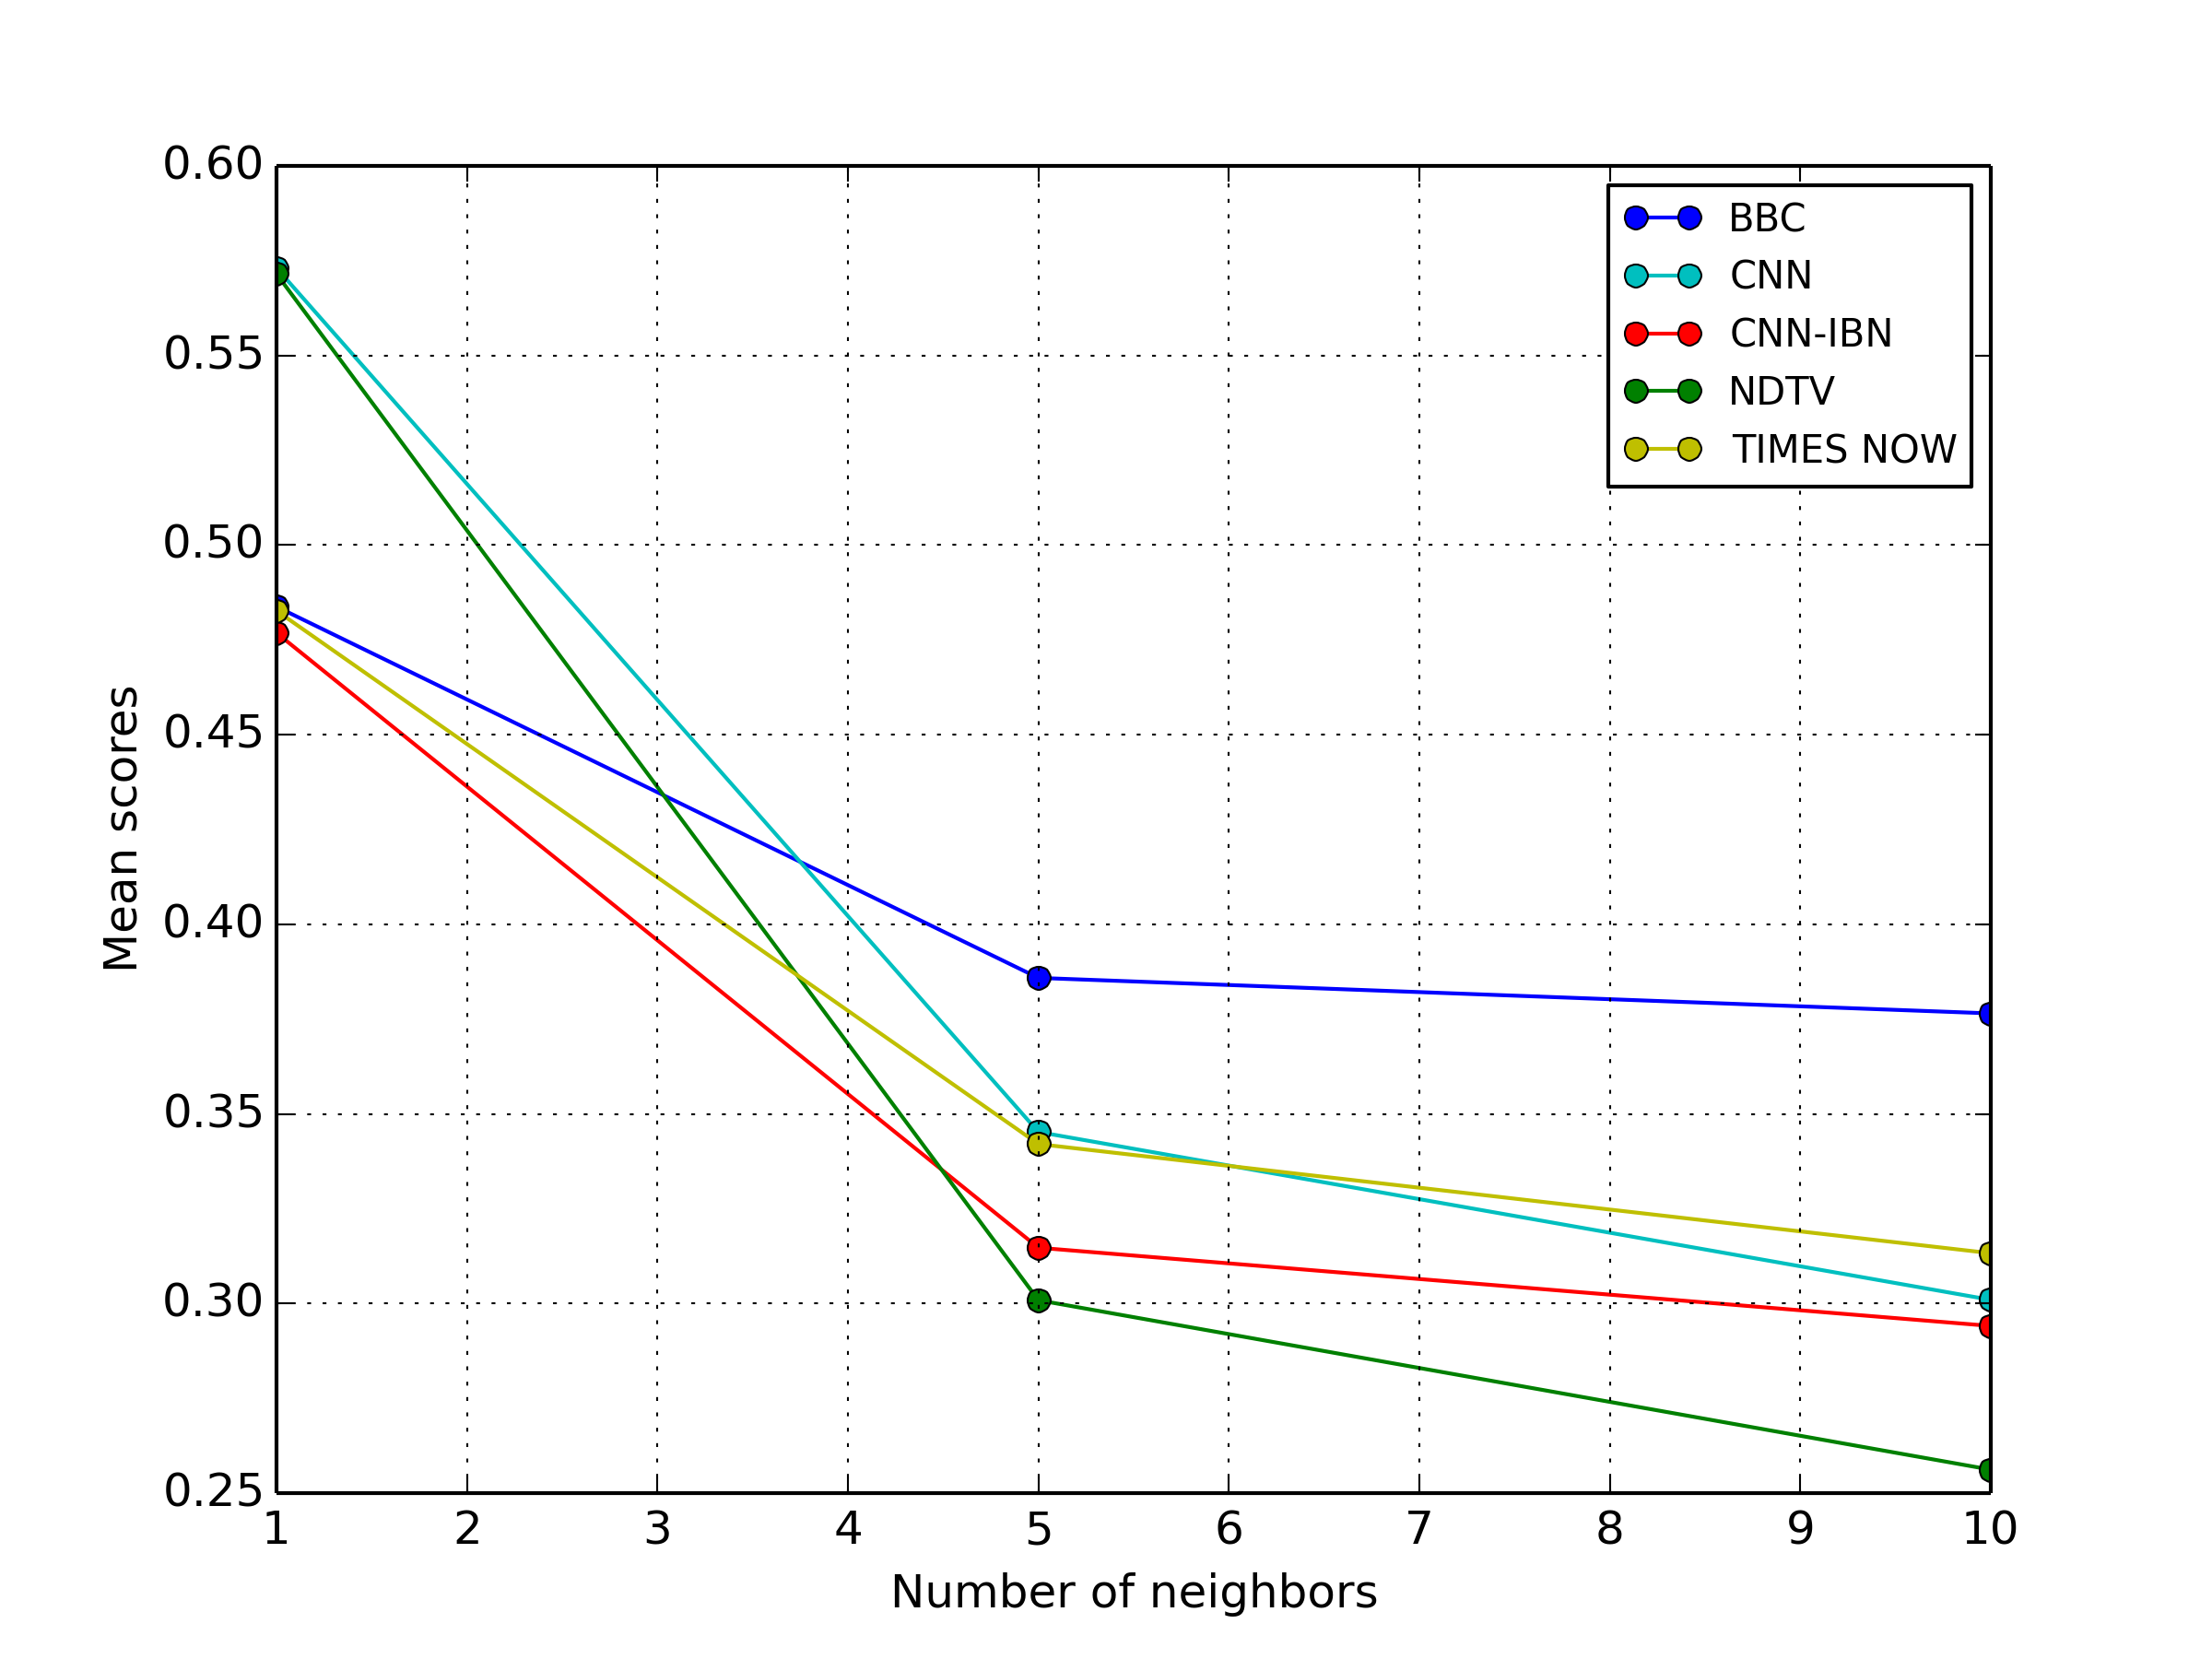
\includegraphics[width=\textwidth]{images/cnn-KNN.png}
		\caption{Качество классификации.}
	\end{subfigure}
	\begin{subfigure}{0.45\textwidth}
		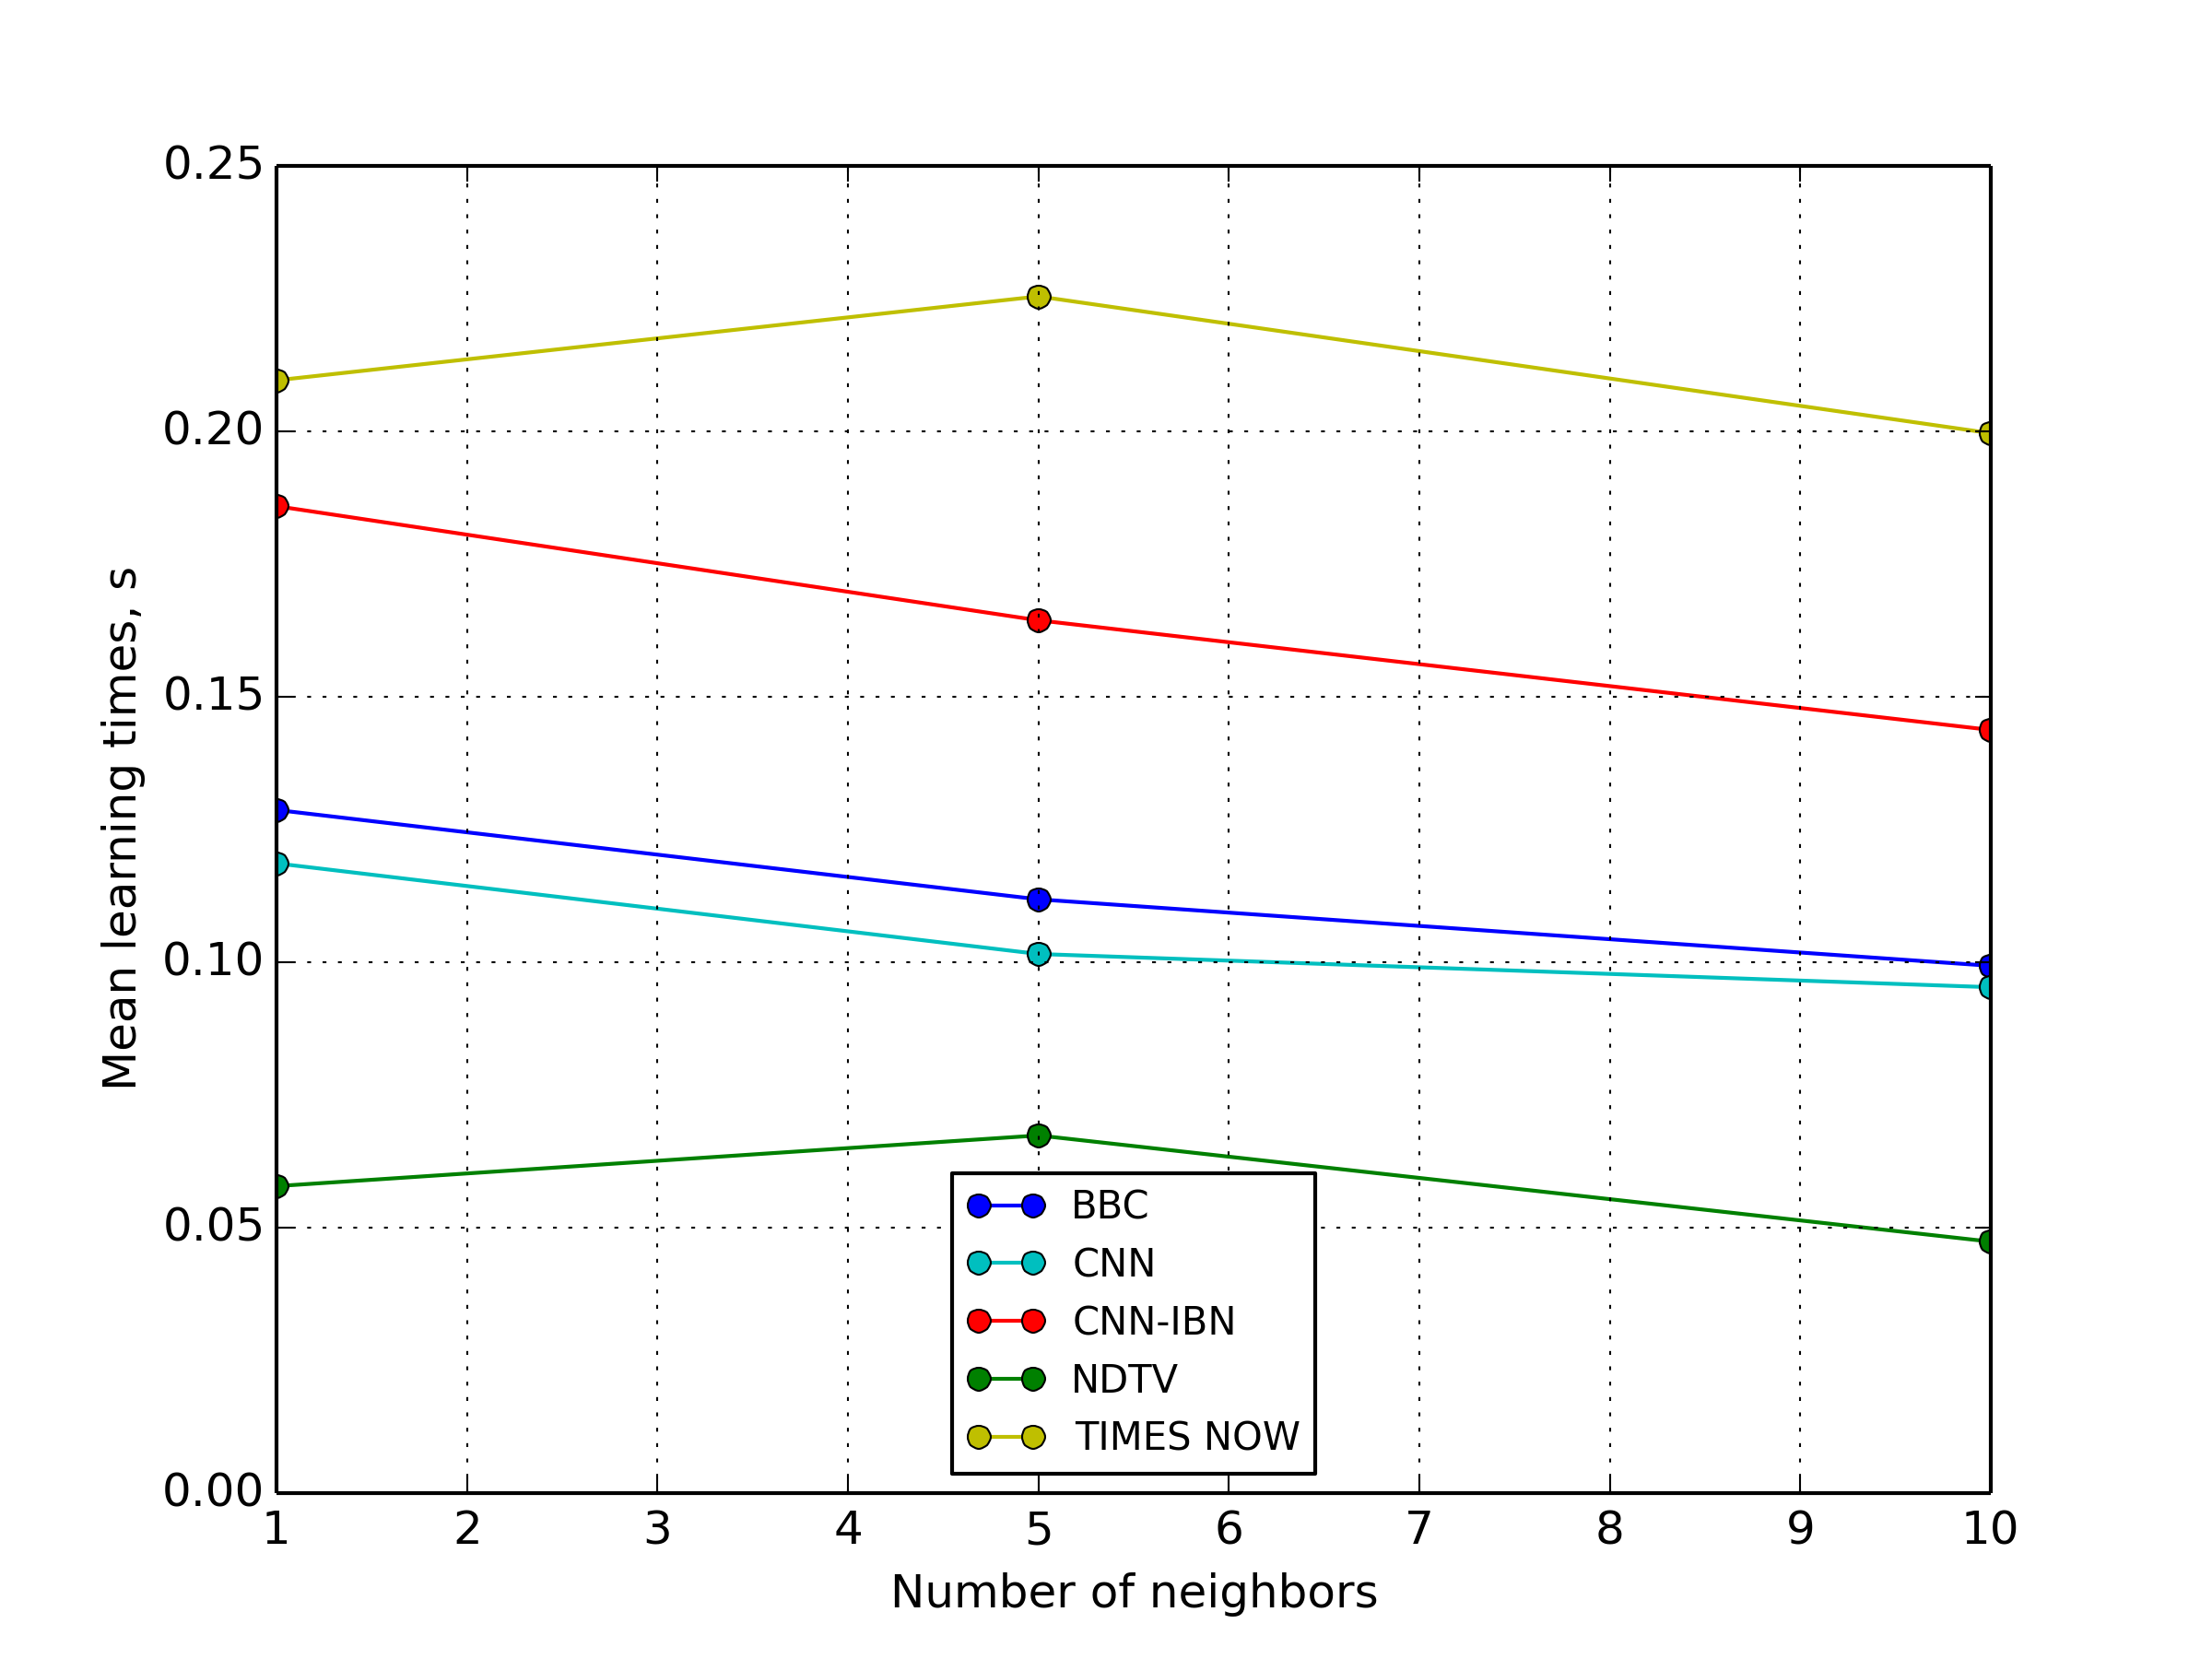
\includegraphics[width=\textwidth]{images/cnn-KNNTime.png}
		\caption{Время обучения.}
	\end{subfigure}
	\caption{Результаты применения CNN для 15-NN.}\label{fig:cnn-knn-results}
\end{figure}

\begin{figure}[h!]
	\centering
	\begin{subfigure}{0.45\textwidth}
		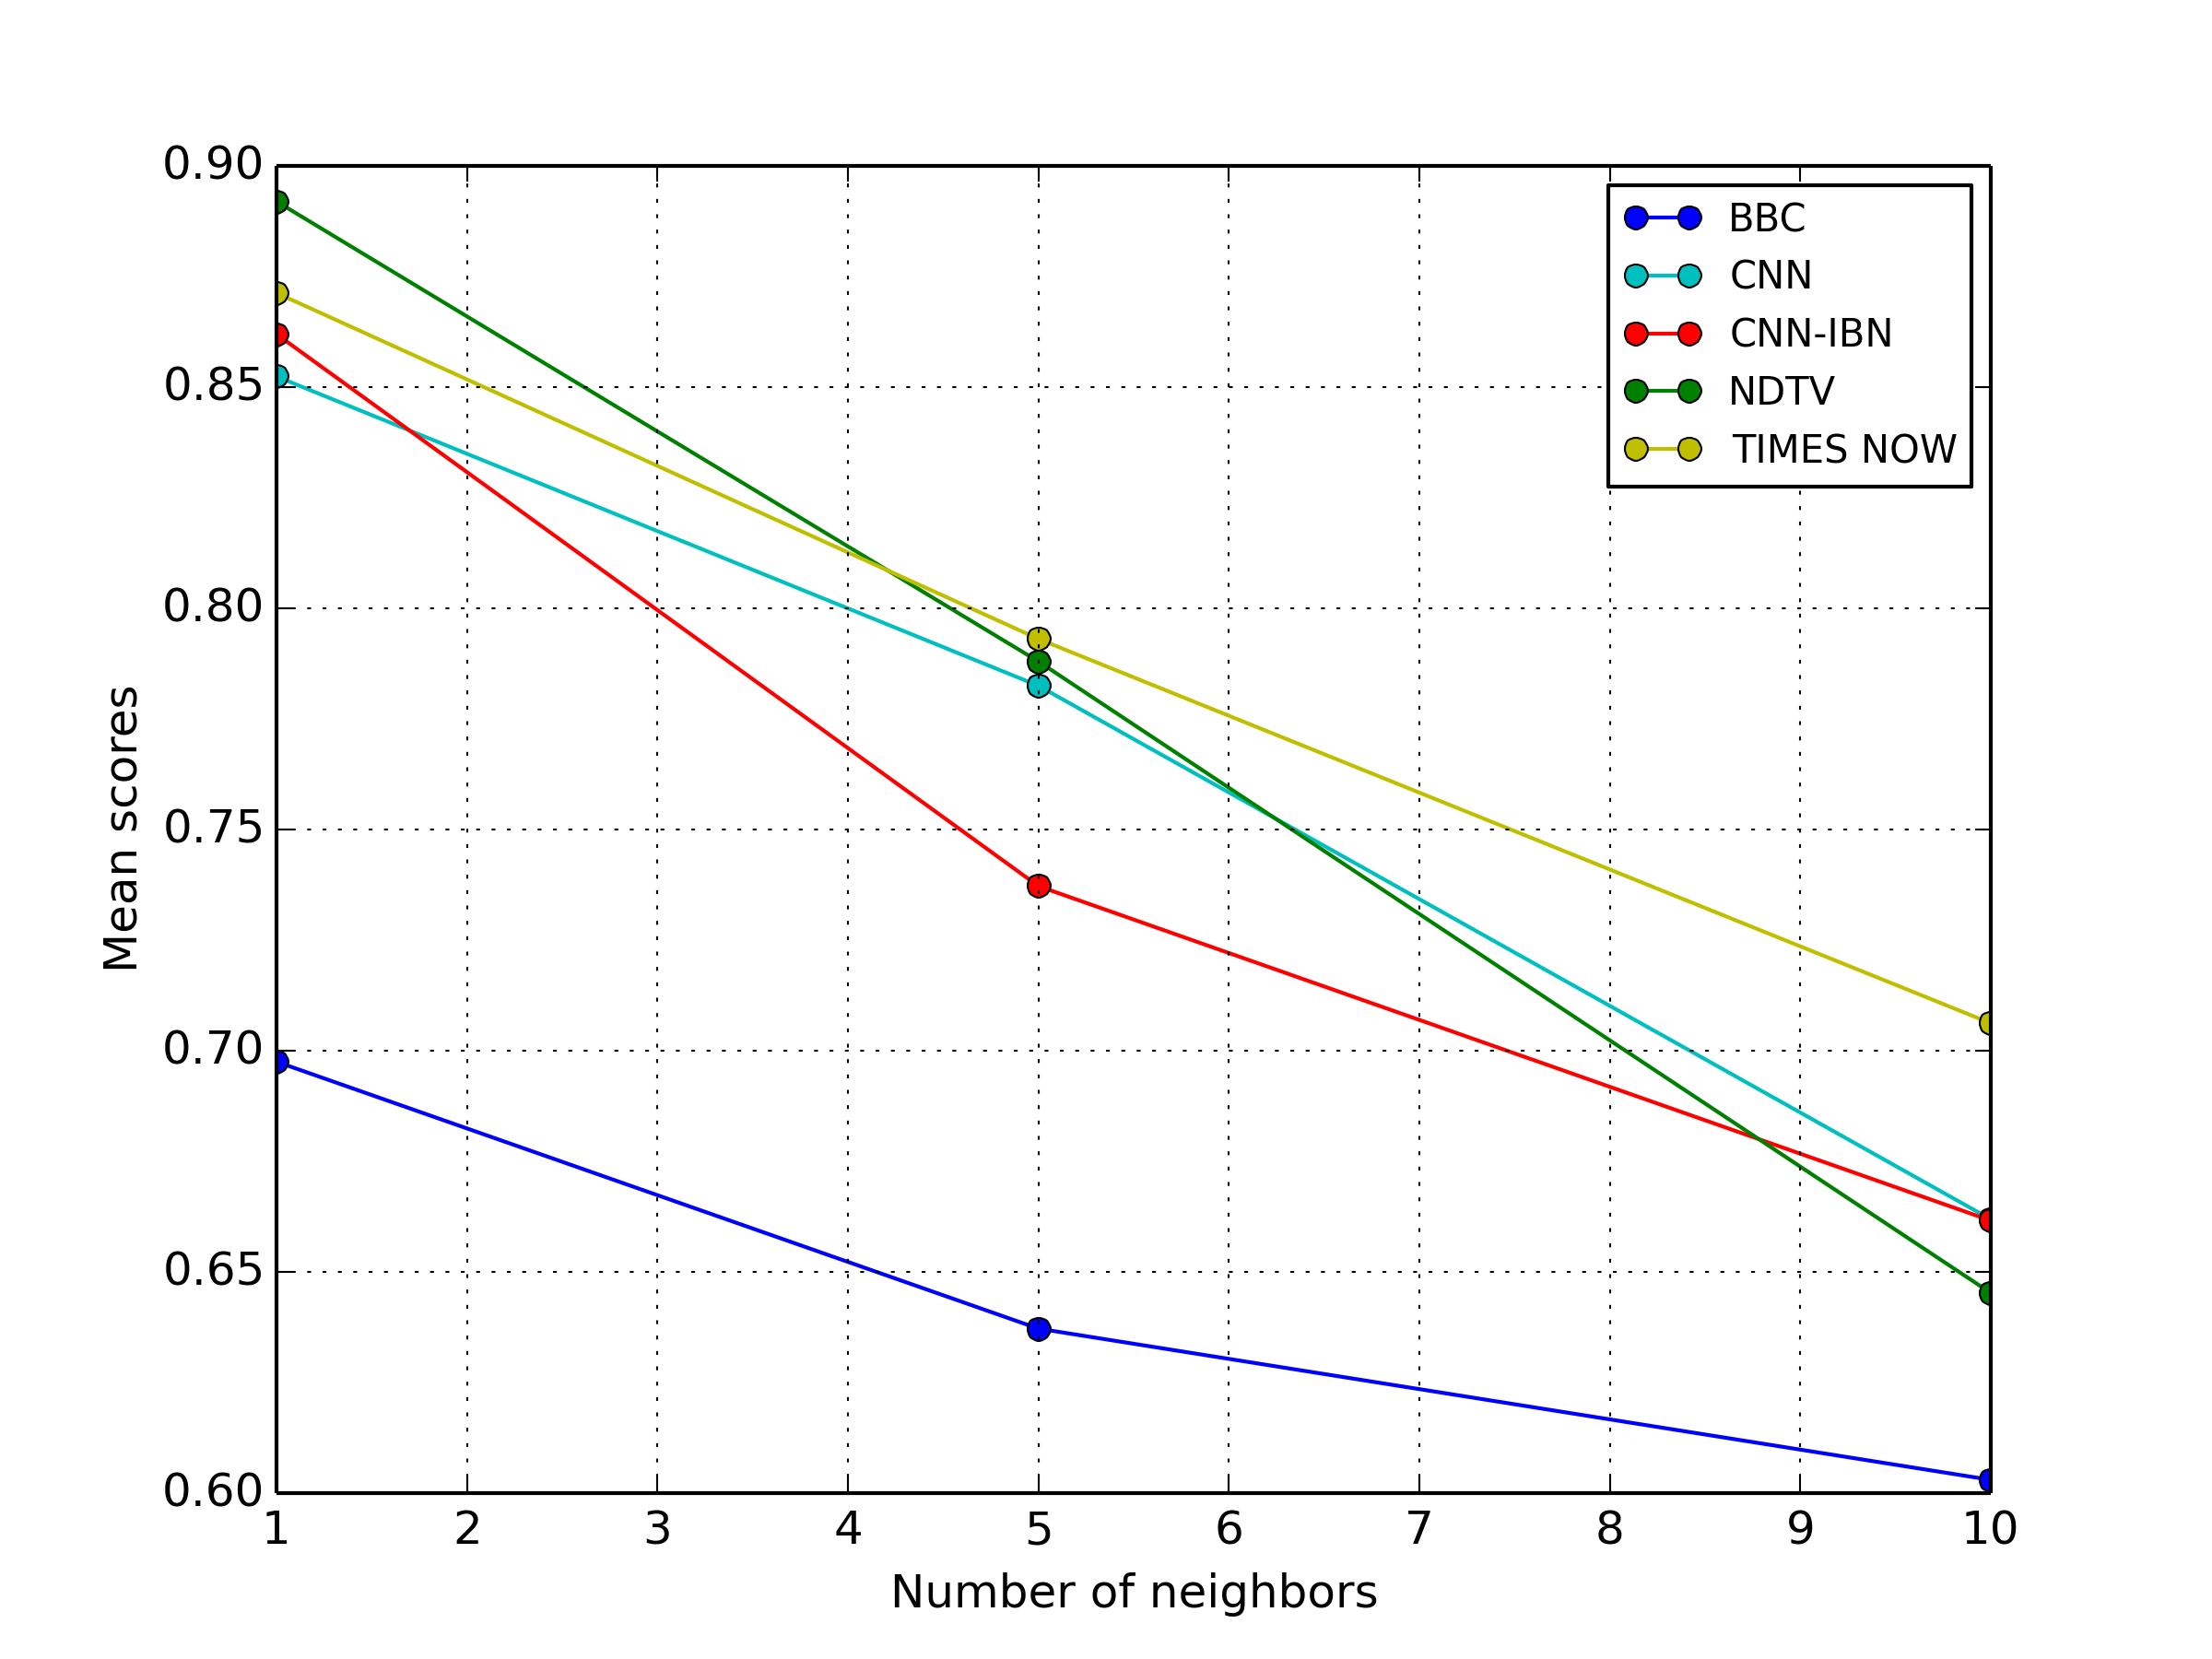
\includegraphics[width=\textwidth]{images/cnn-LDA.png}
		\caption{Качество классификации.}
	\end{subfigure}
	\begin{subfigure}{0.45\textwidth}
		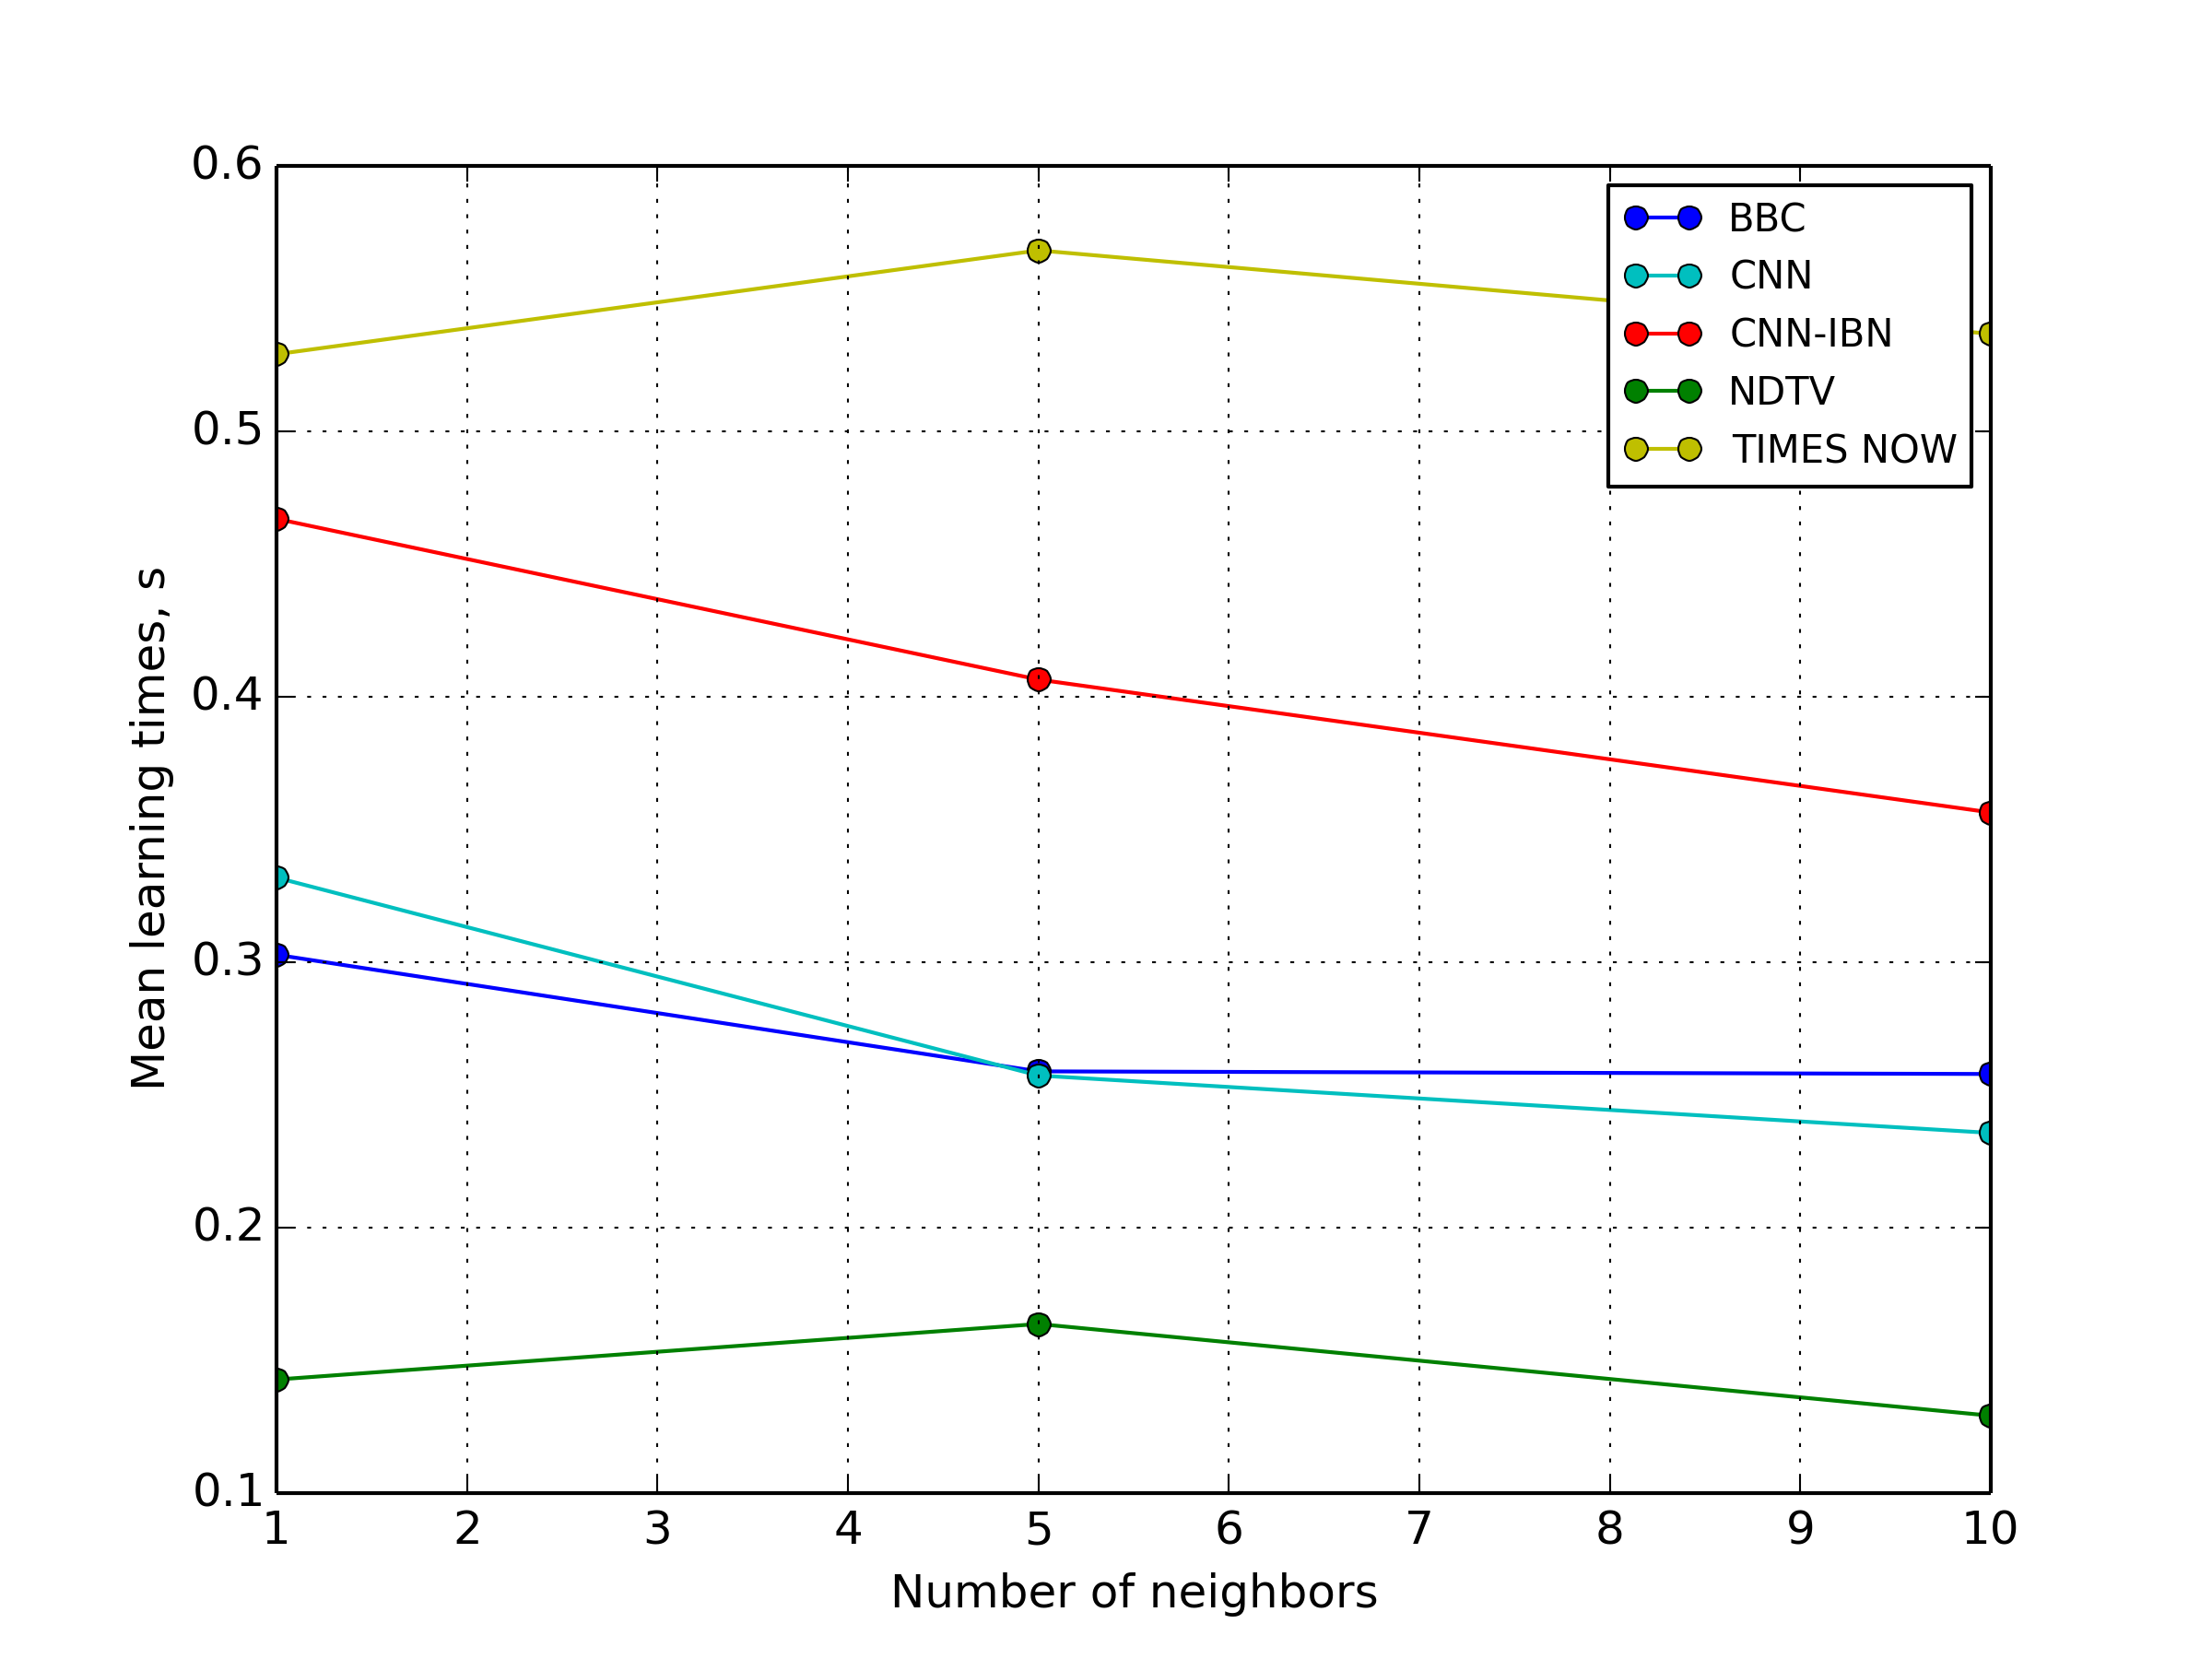
\includegraphics[width=\textwidth]{images/cnn-LDATime.png}
		\caption{Время обучения.}
	\end{subfigure}
	\caption{Результаты применения CNN для LDA.}\label{fig:cnn-lda-results}
\end{figure}

\begin{figure}[h!]
	\centering
	\begin{subfigure}{0.45\textwidth}
		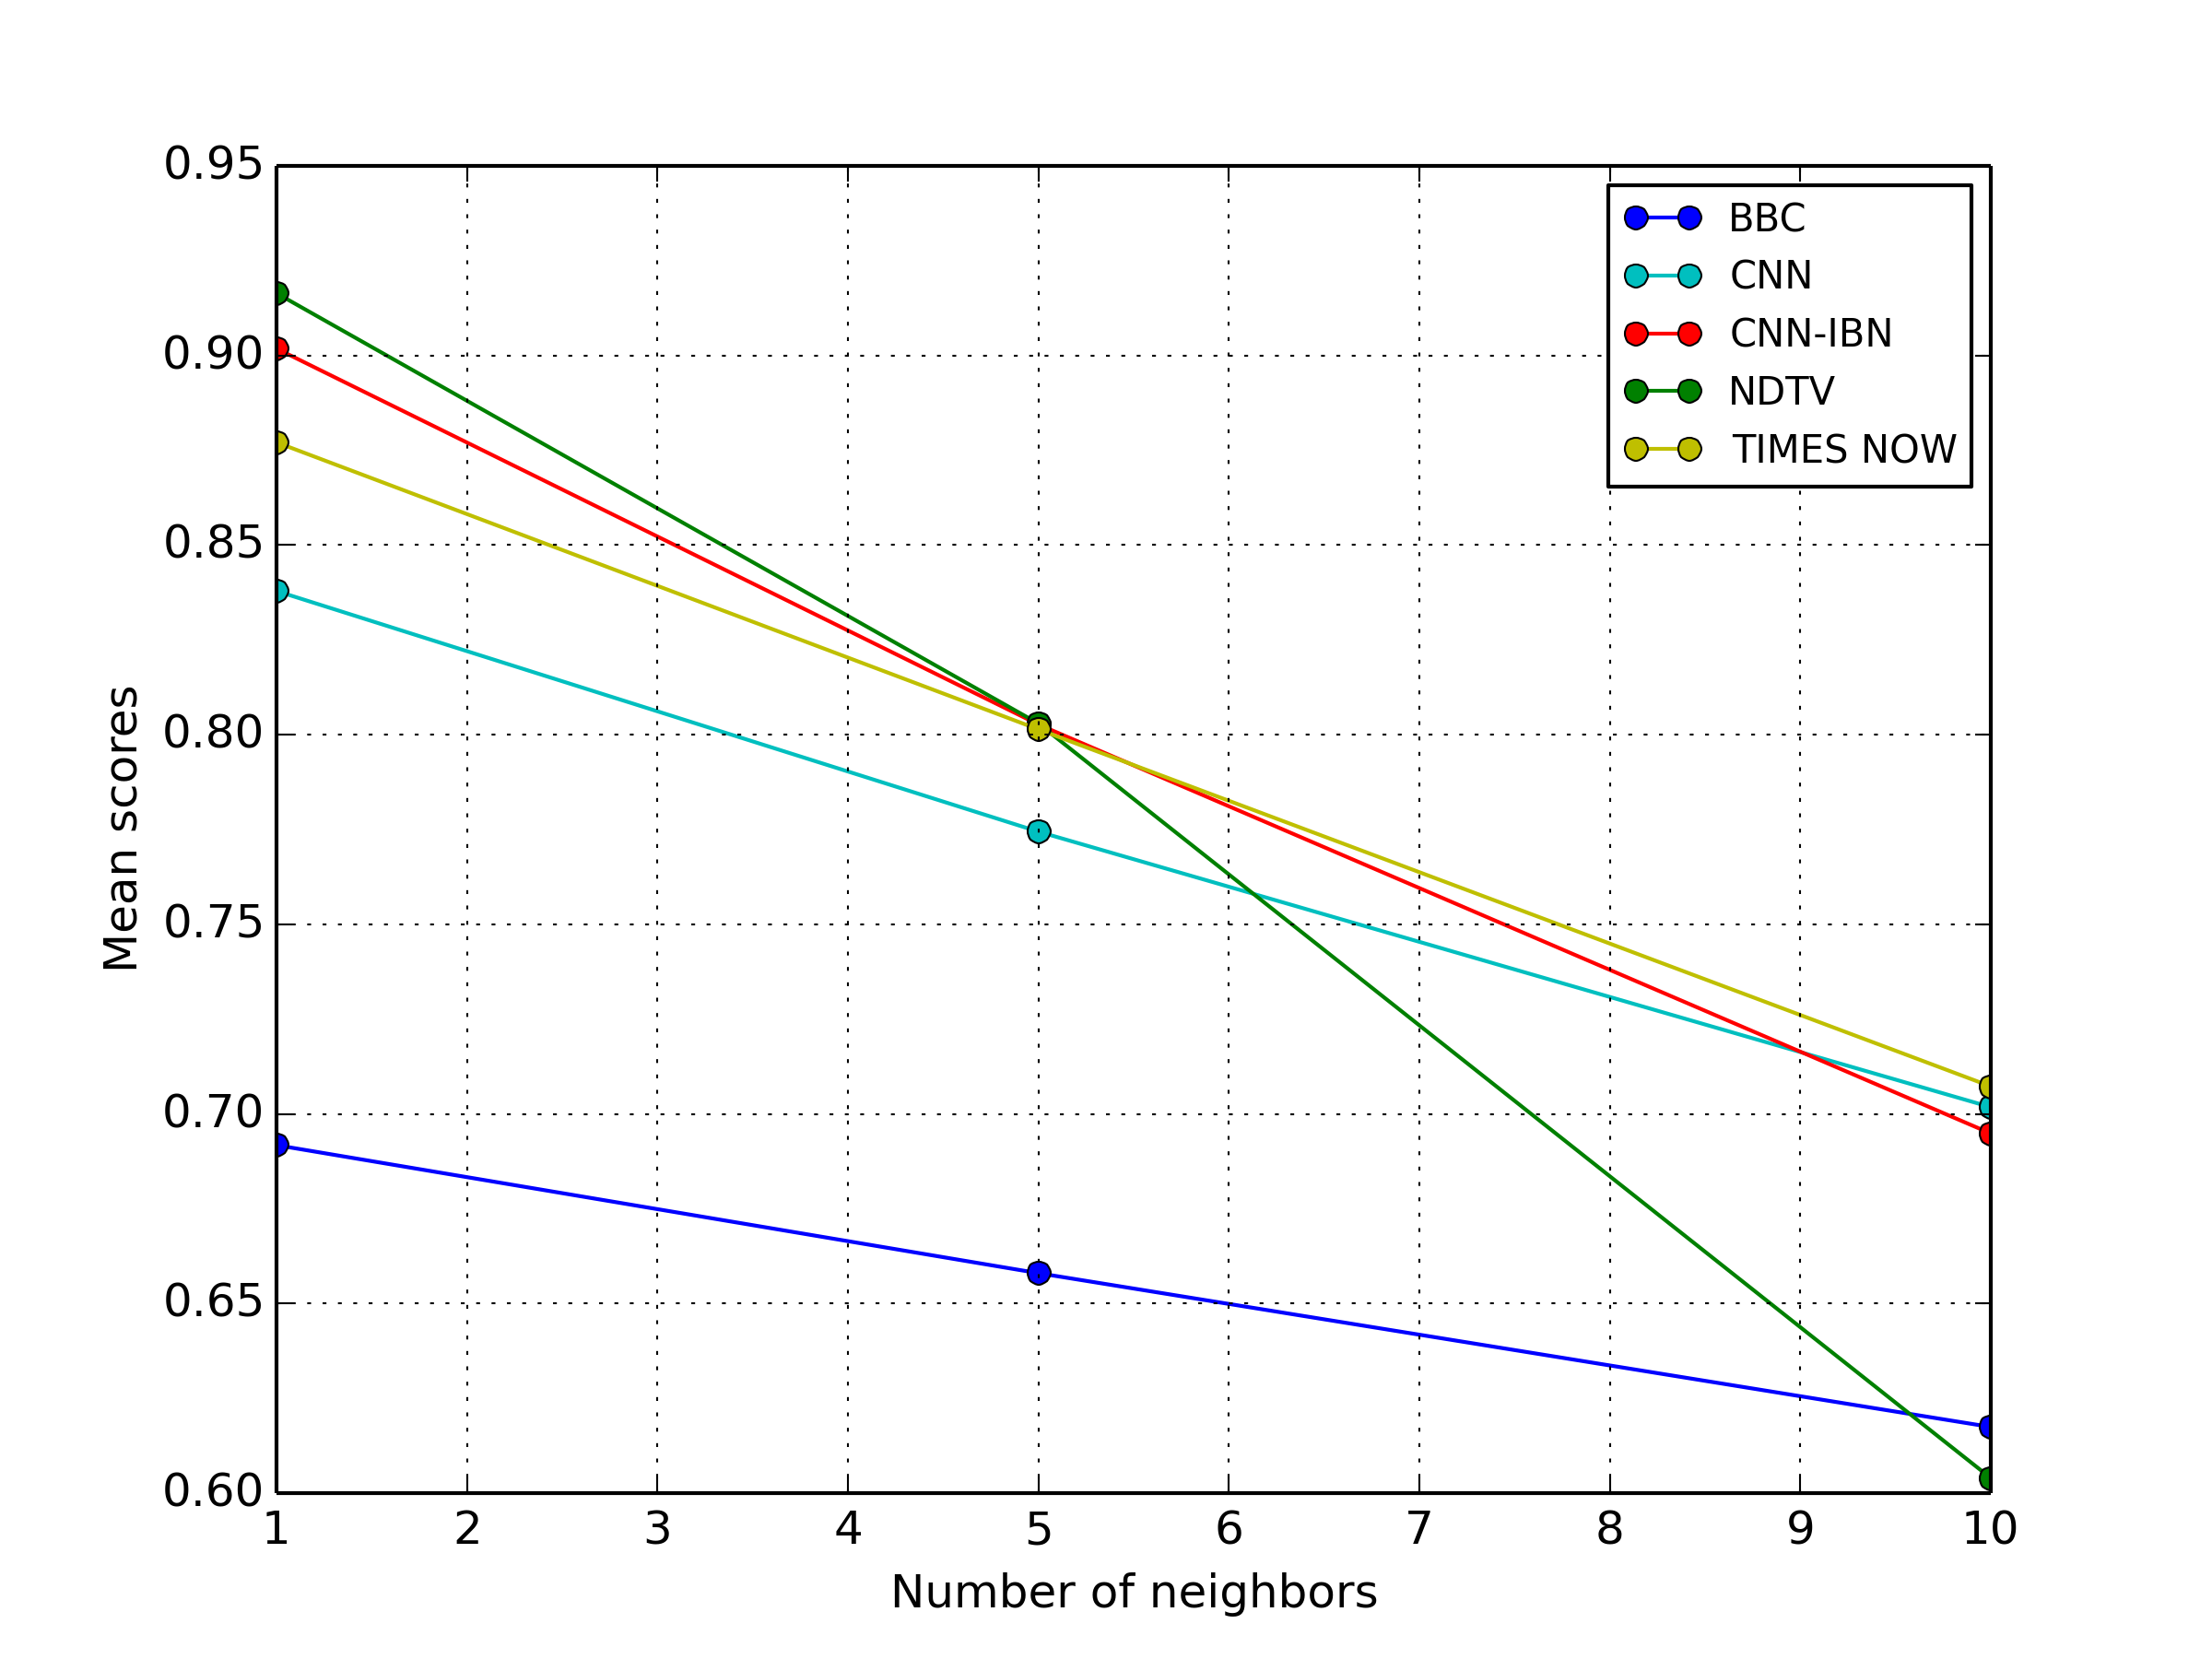
\includegraphics[width=\textwidth]{images/cnn-SVM.png}
		\caption{Качество классификации.}
	\end{subfigure}
	\begin{subfigure}{0.45\textwidth}
		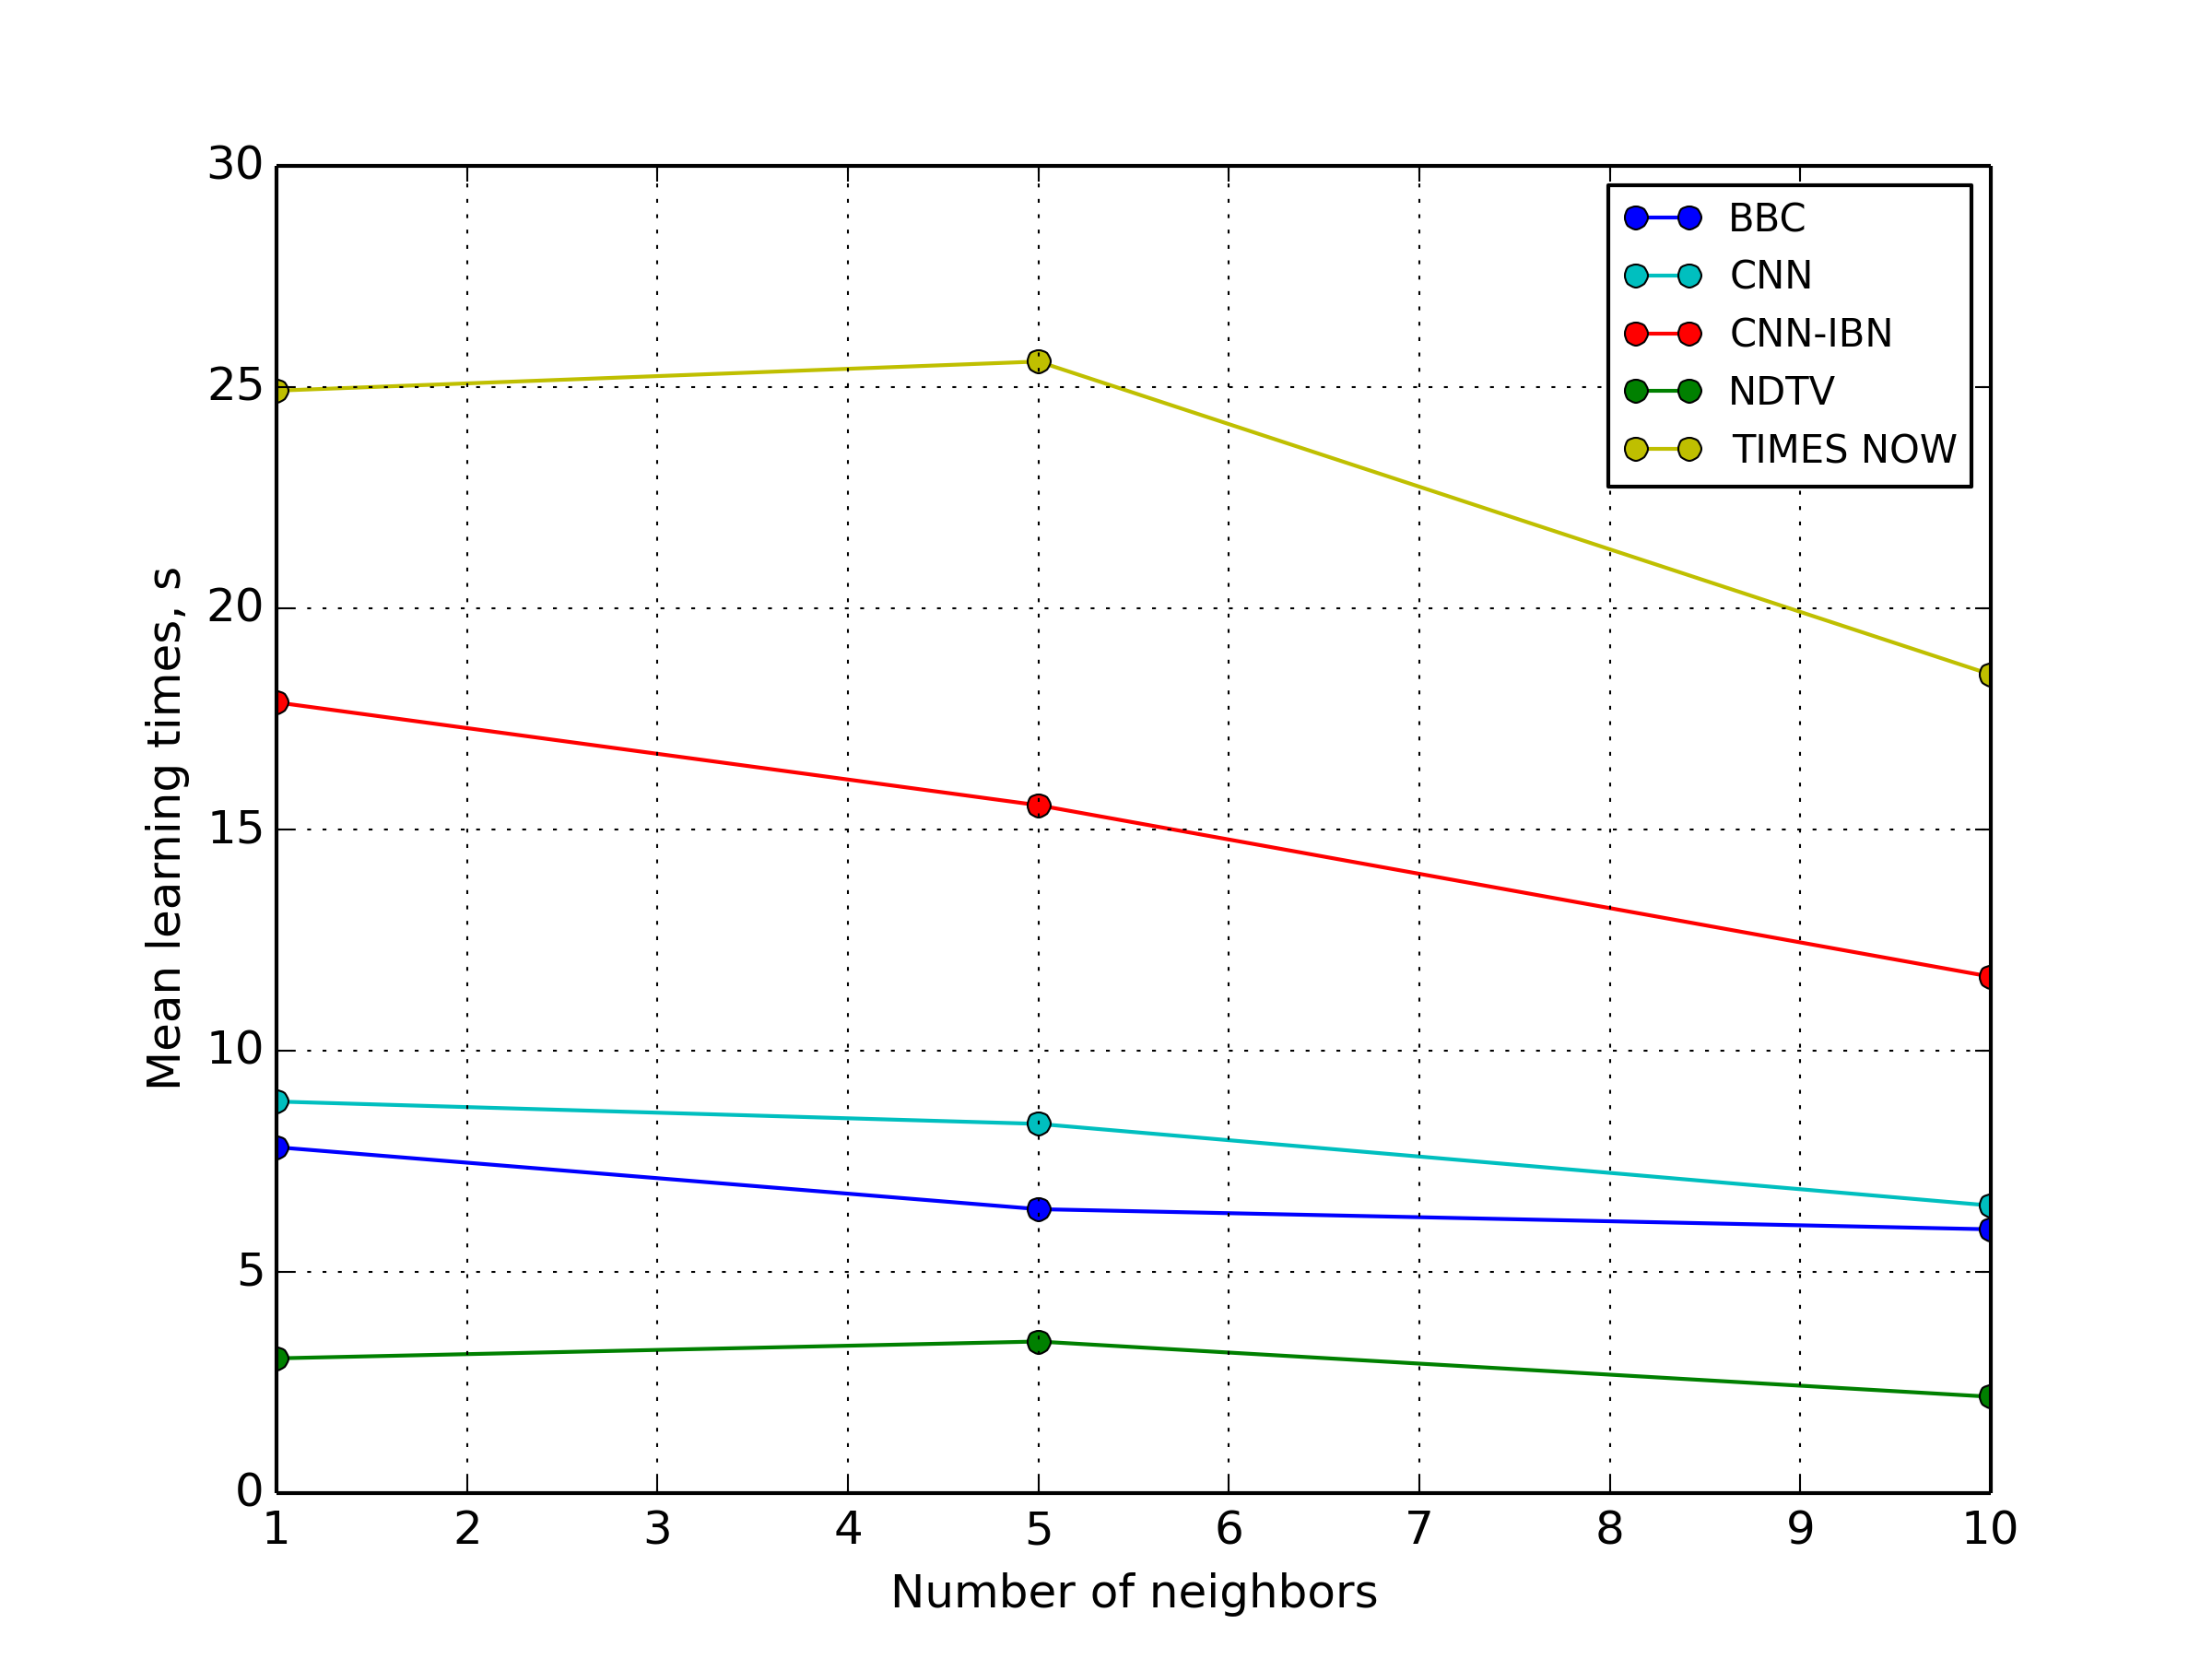
\includegraphics[width=\textwidth]{images/cnn-SVMTime.png}
		\caption{Время обучения.}
	\end{subfigure}
	\caption{Результаты применения CNN для SVM.}\label{fig:cnn-svm-results}
\end{figure}

\begin{figure}[h!]
	\centering
	\begin{subfigure}{0.45\textwidth}
		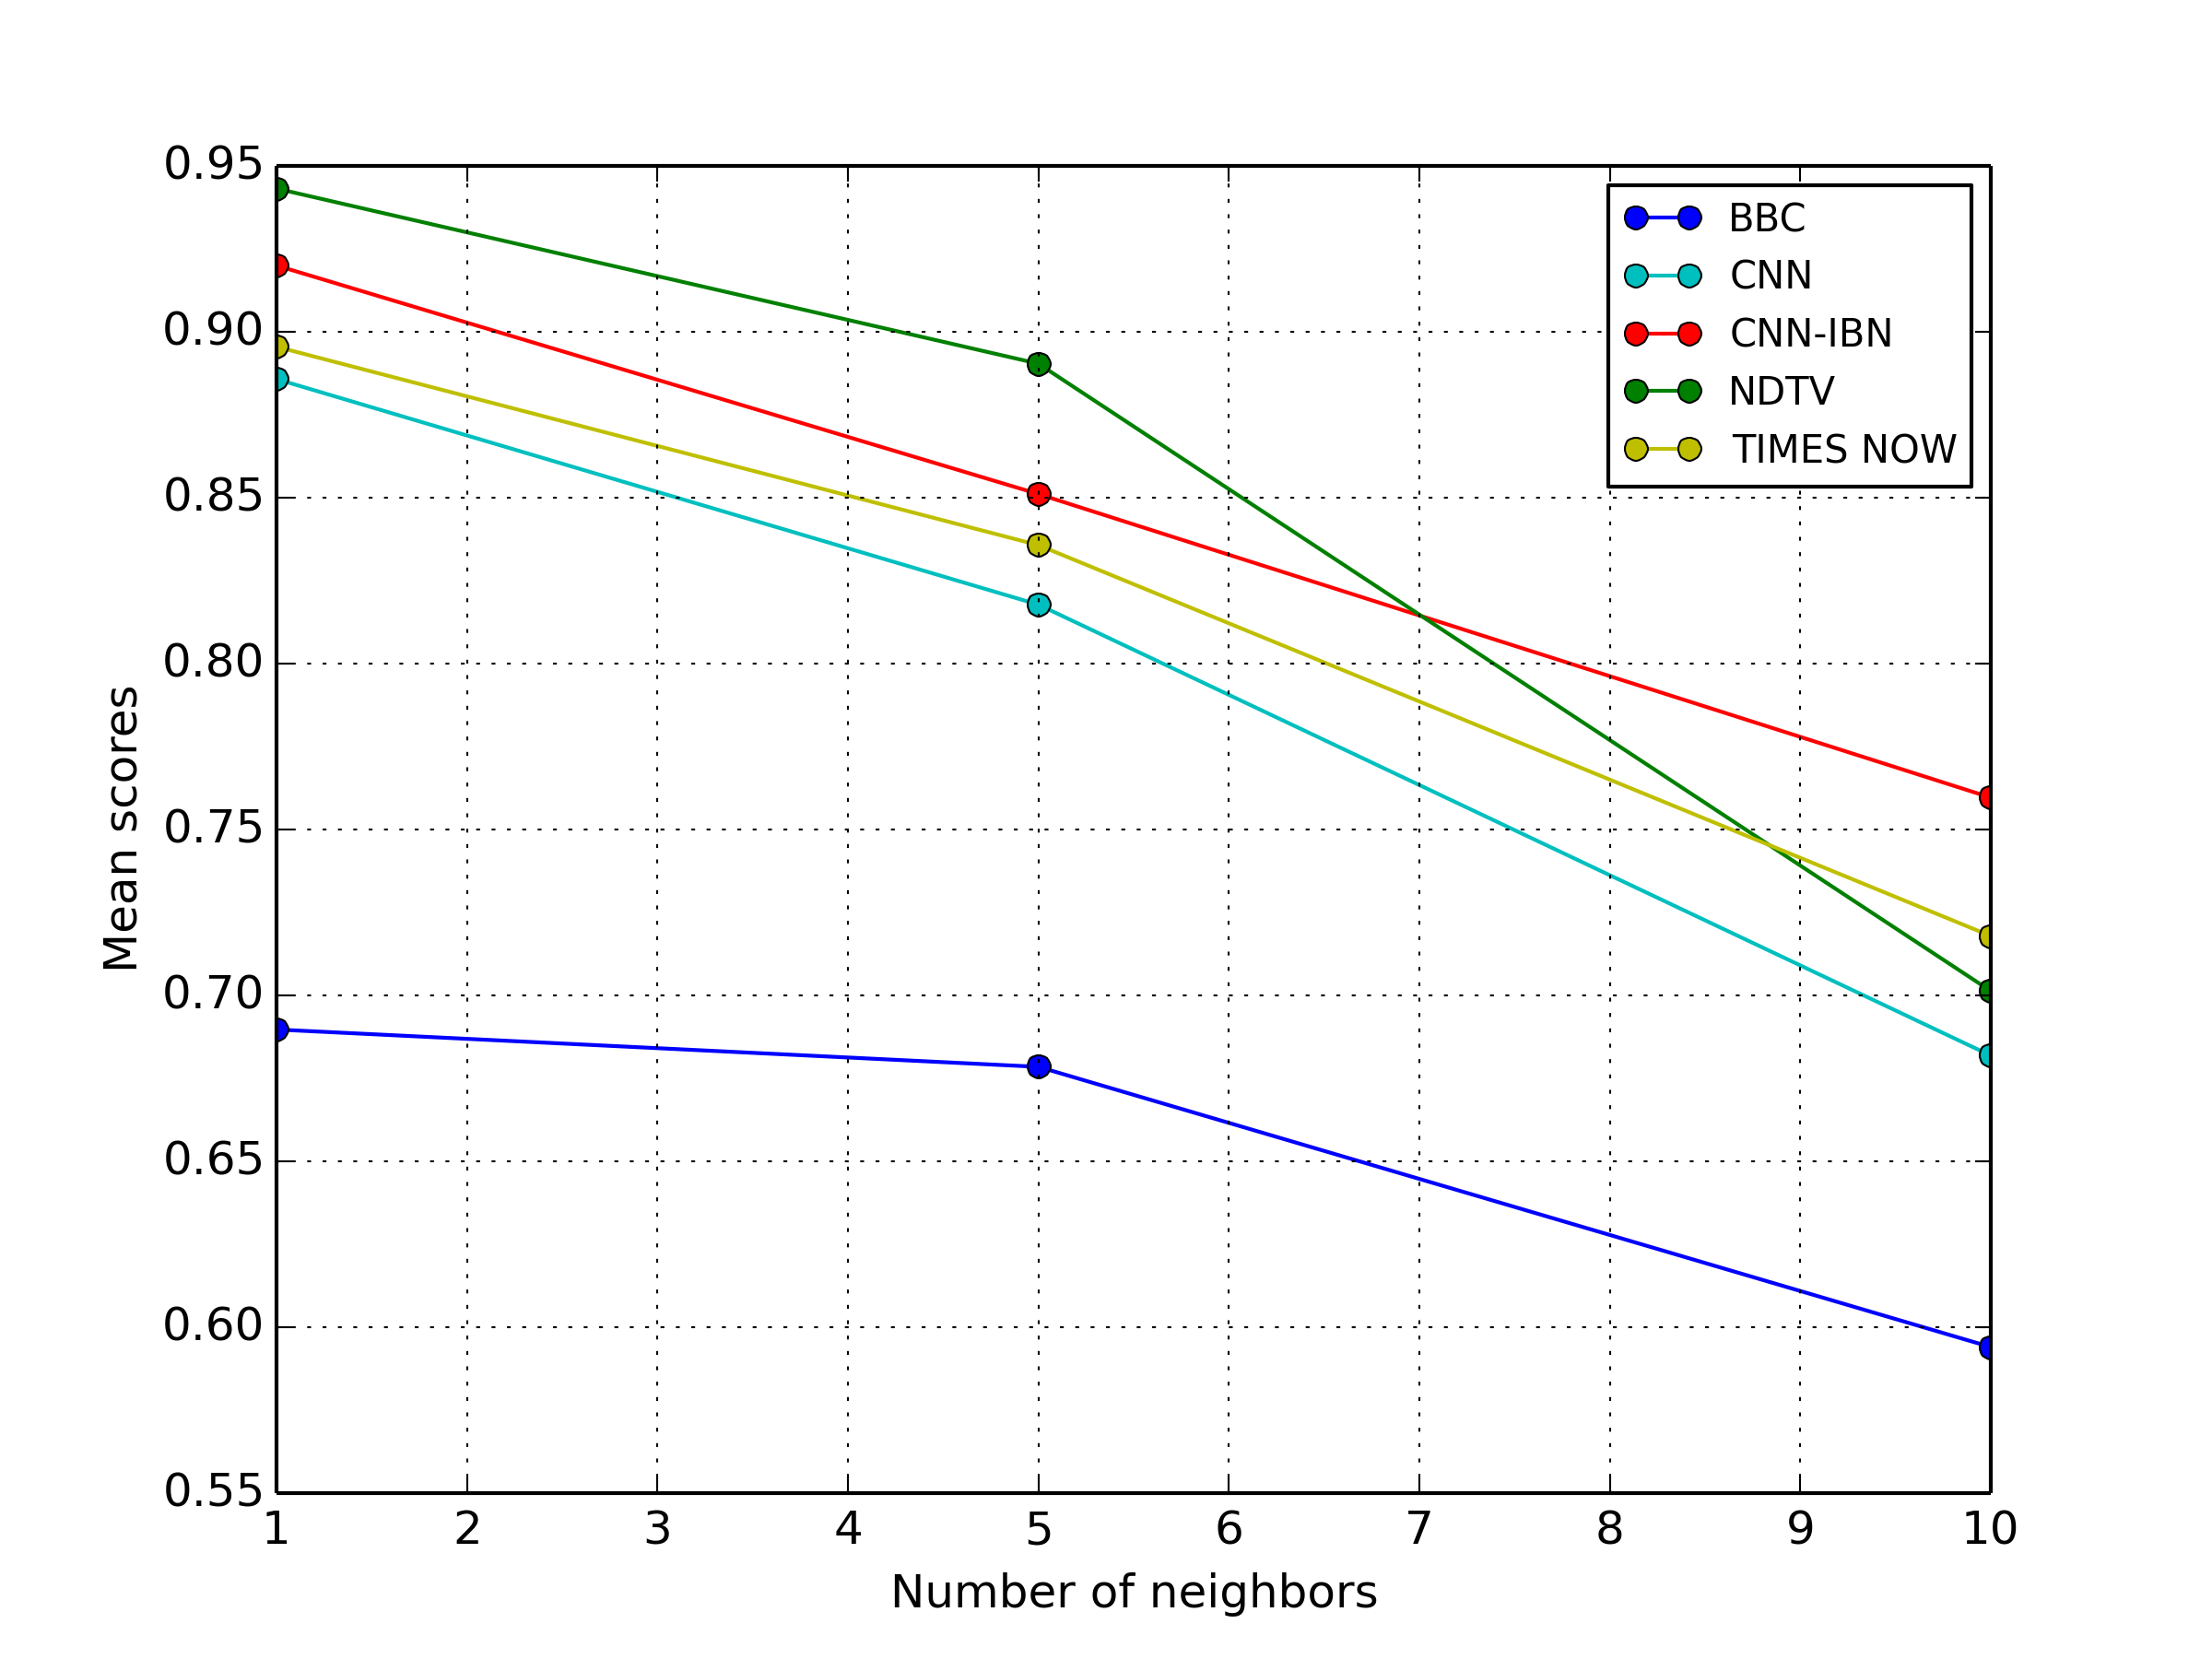
\includegraphics[width=\textwidth]{images/cnn-randforest.png}
		\caption{Качество классификации.}
	\end{subfigure}
	\begin{subfigure}{0.45\textwidth}
		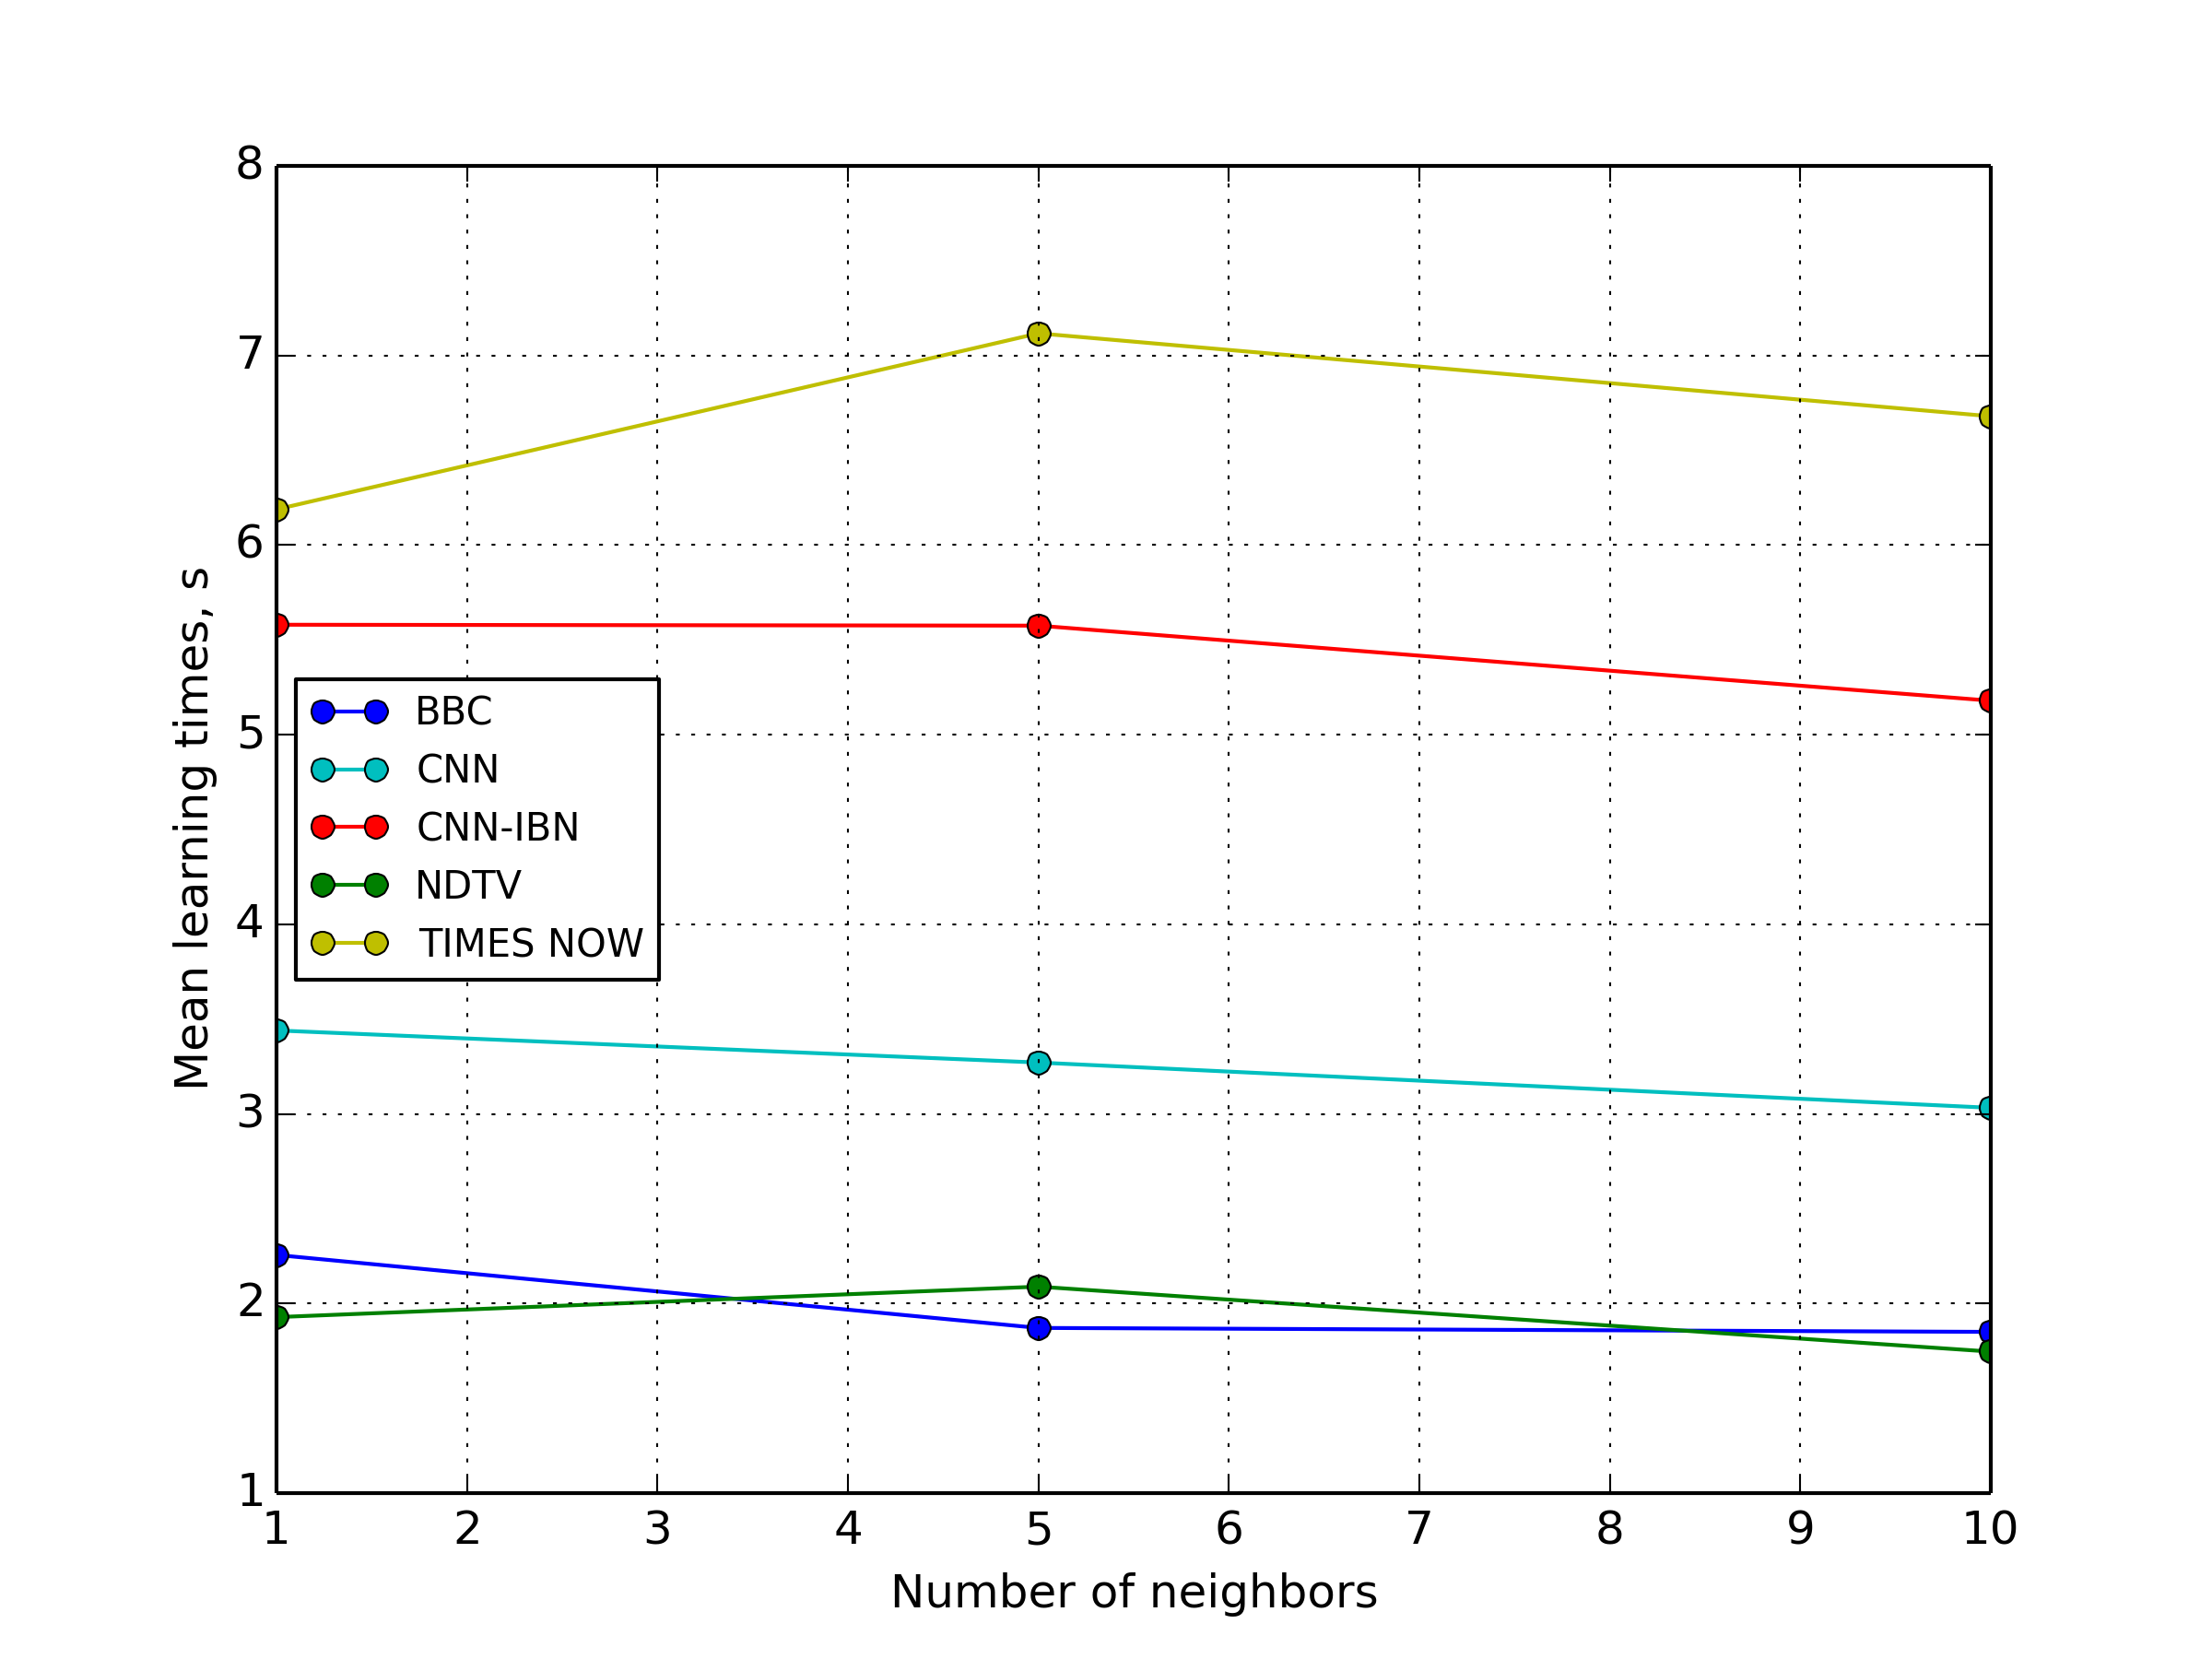
\includegraphics[width=\textwidth]{images/cnn-randforestTime.png}
		\caption{Время обучения.}
	\end{subfigure}
	\caption{Результаты применения CNN для Random forest.}\label{fig:cnn-rf-results}
\end{figure}

\begin{figure}
	\centering
	\begin{subfigure}{0.45\textwidth}
		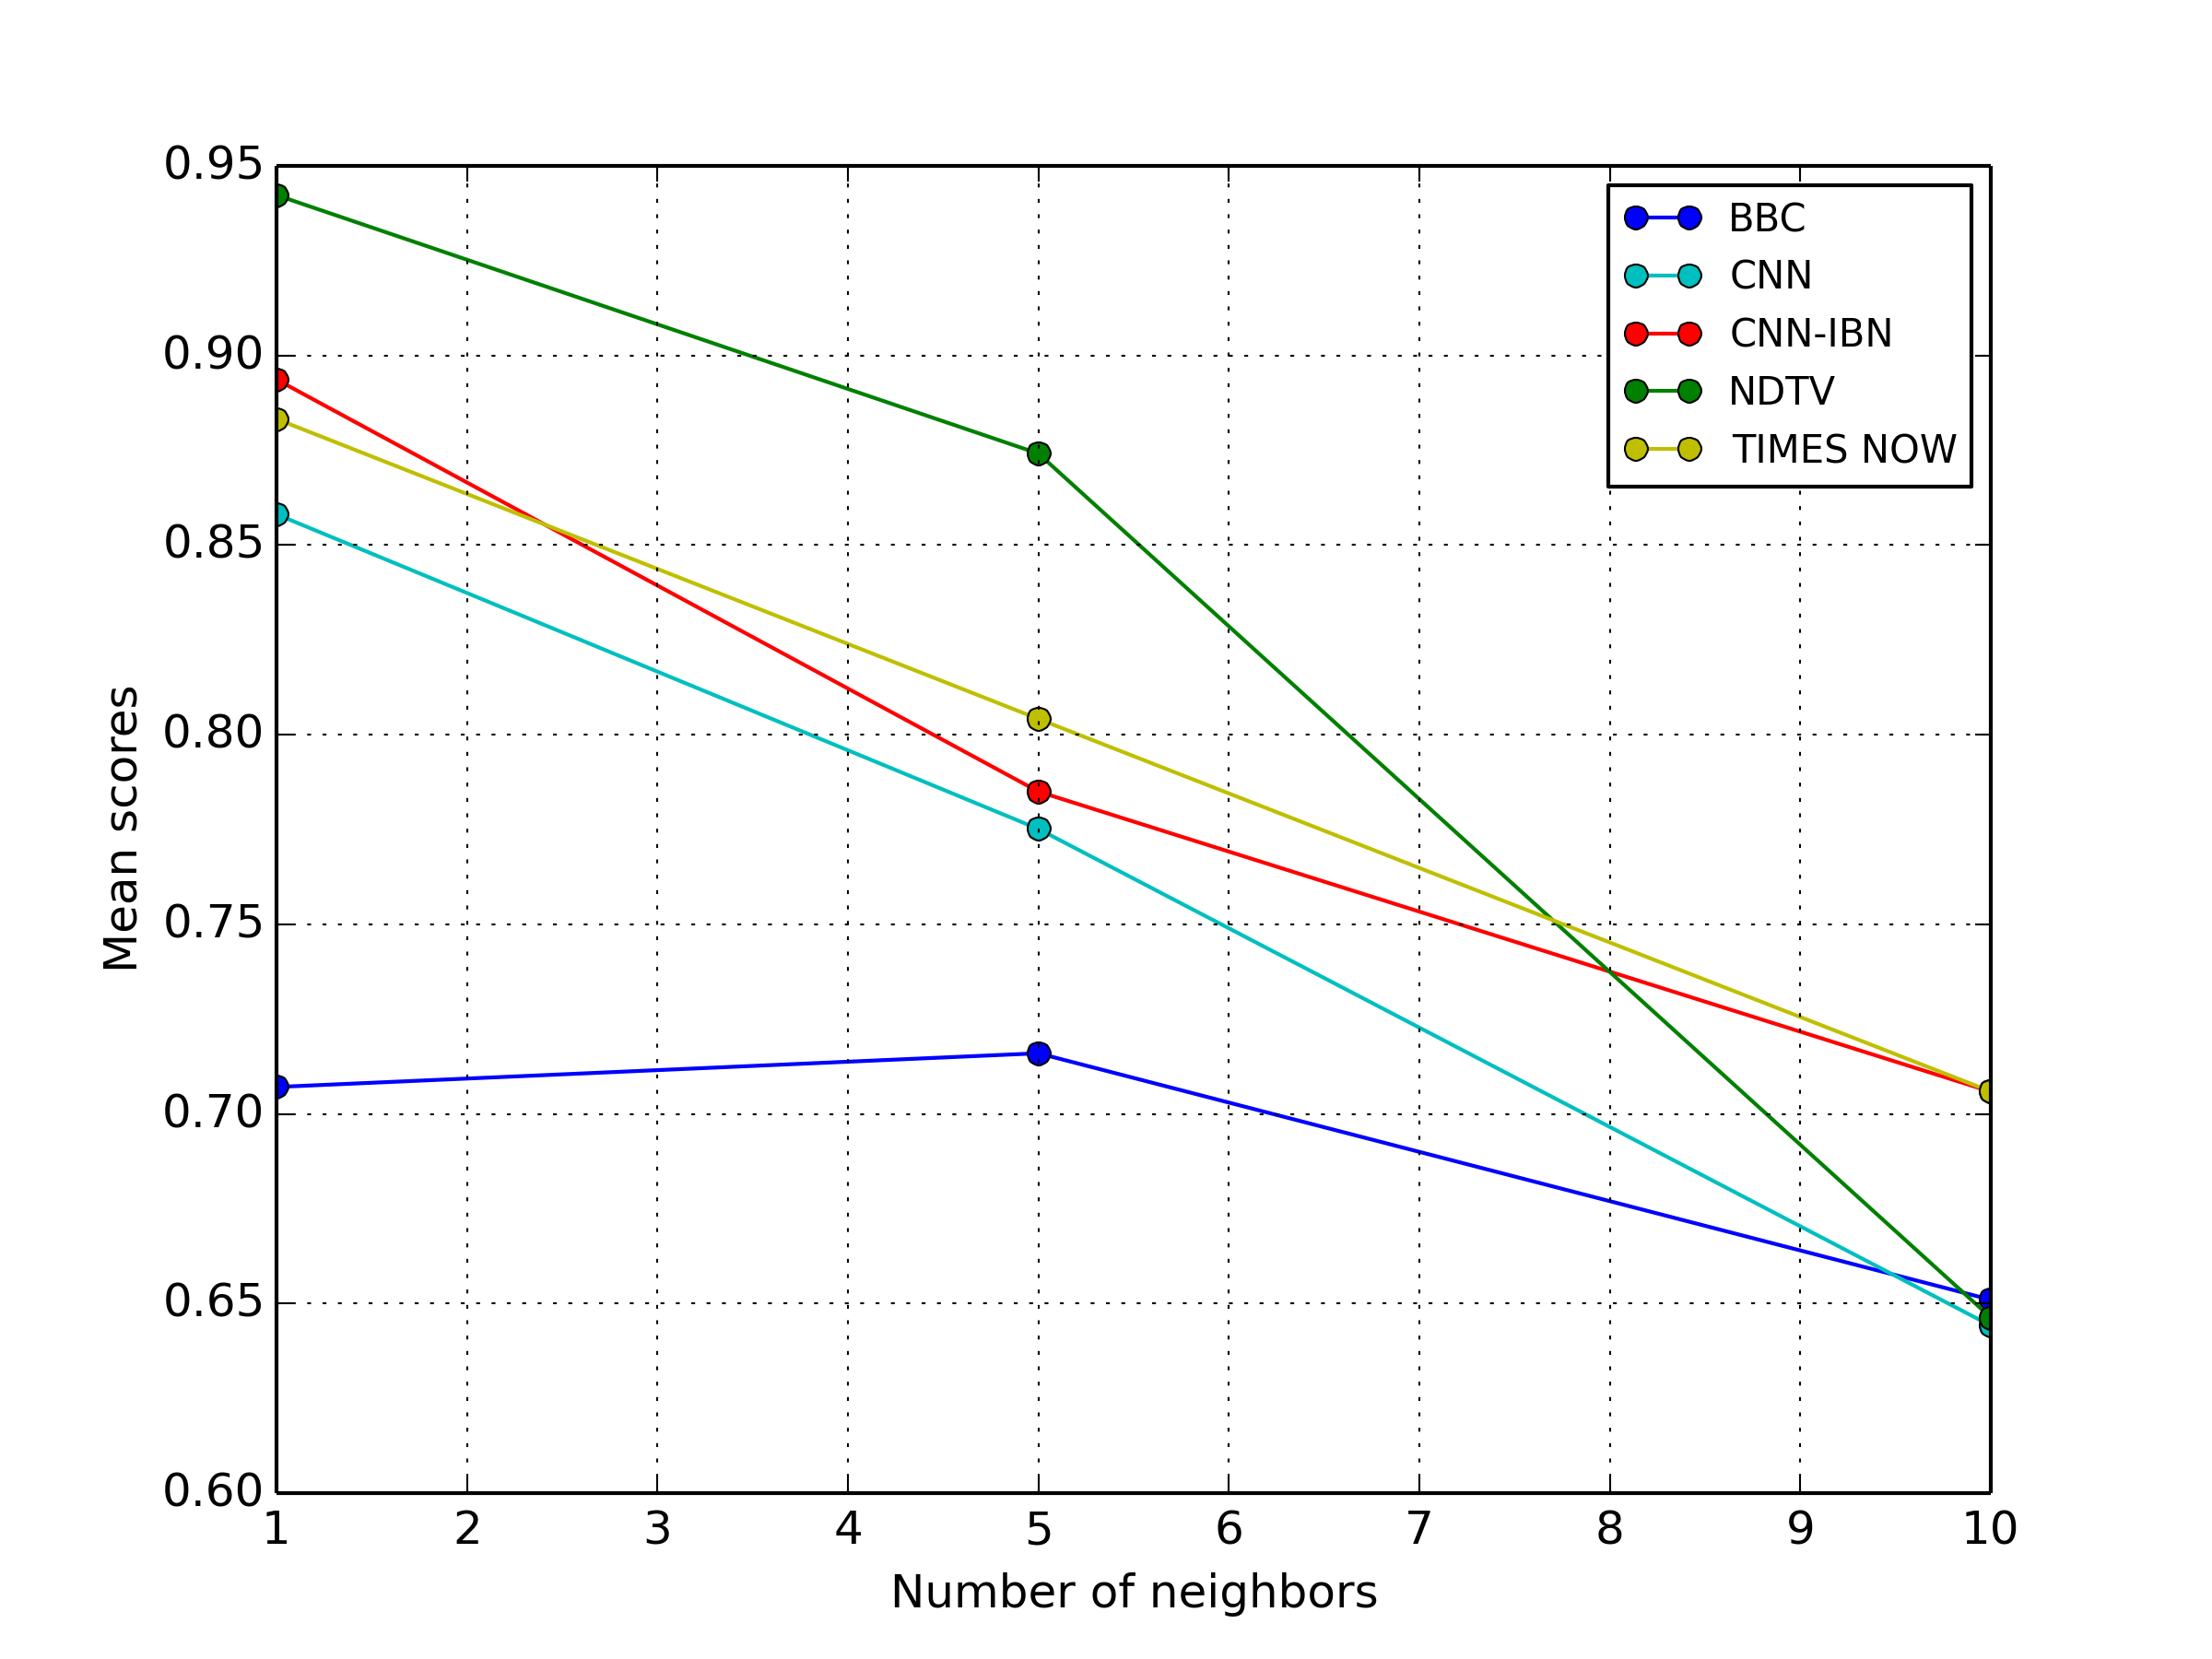
\includegraphics[width=\textwidth]{images/cnn-gradboosting.png}
		\caption{Качество классификации.}
	\end{subfigure}
	\begin{subfigure}{0.45\textwidth}
		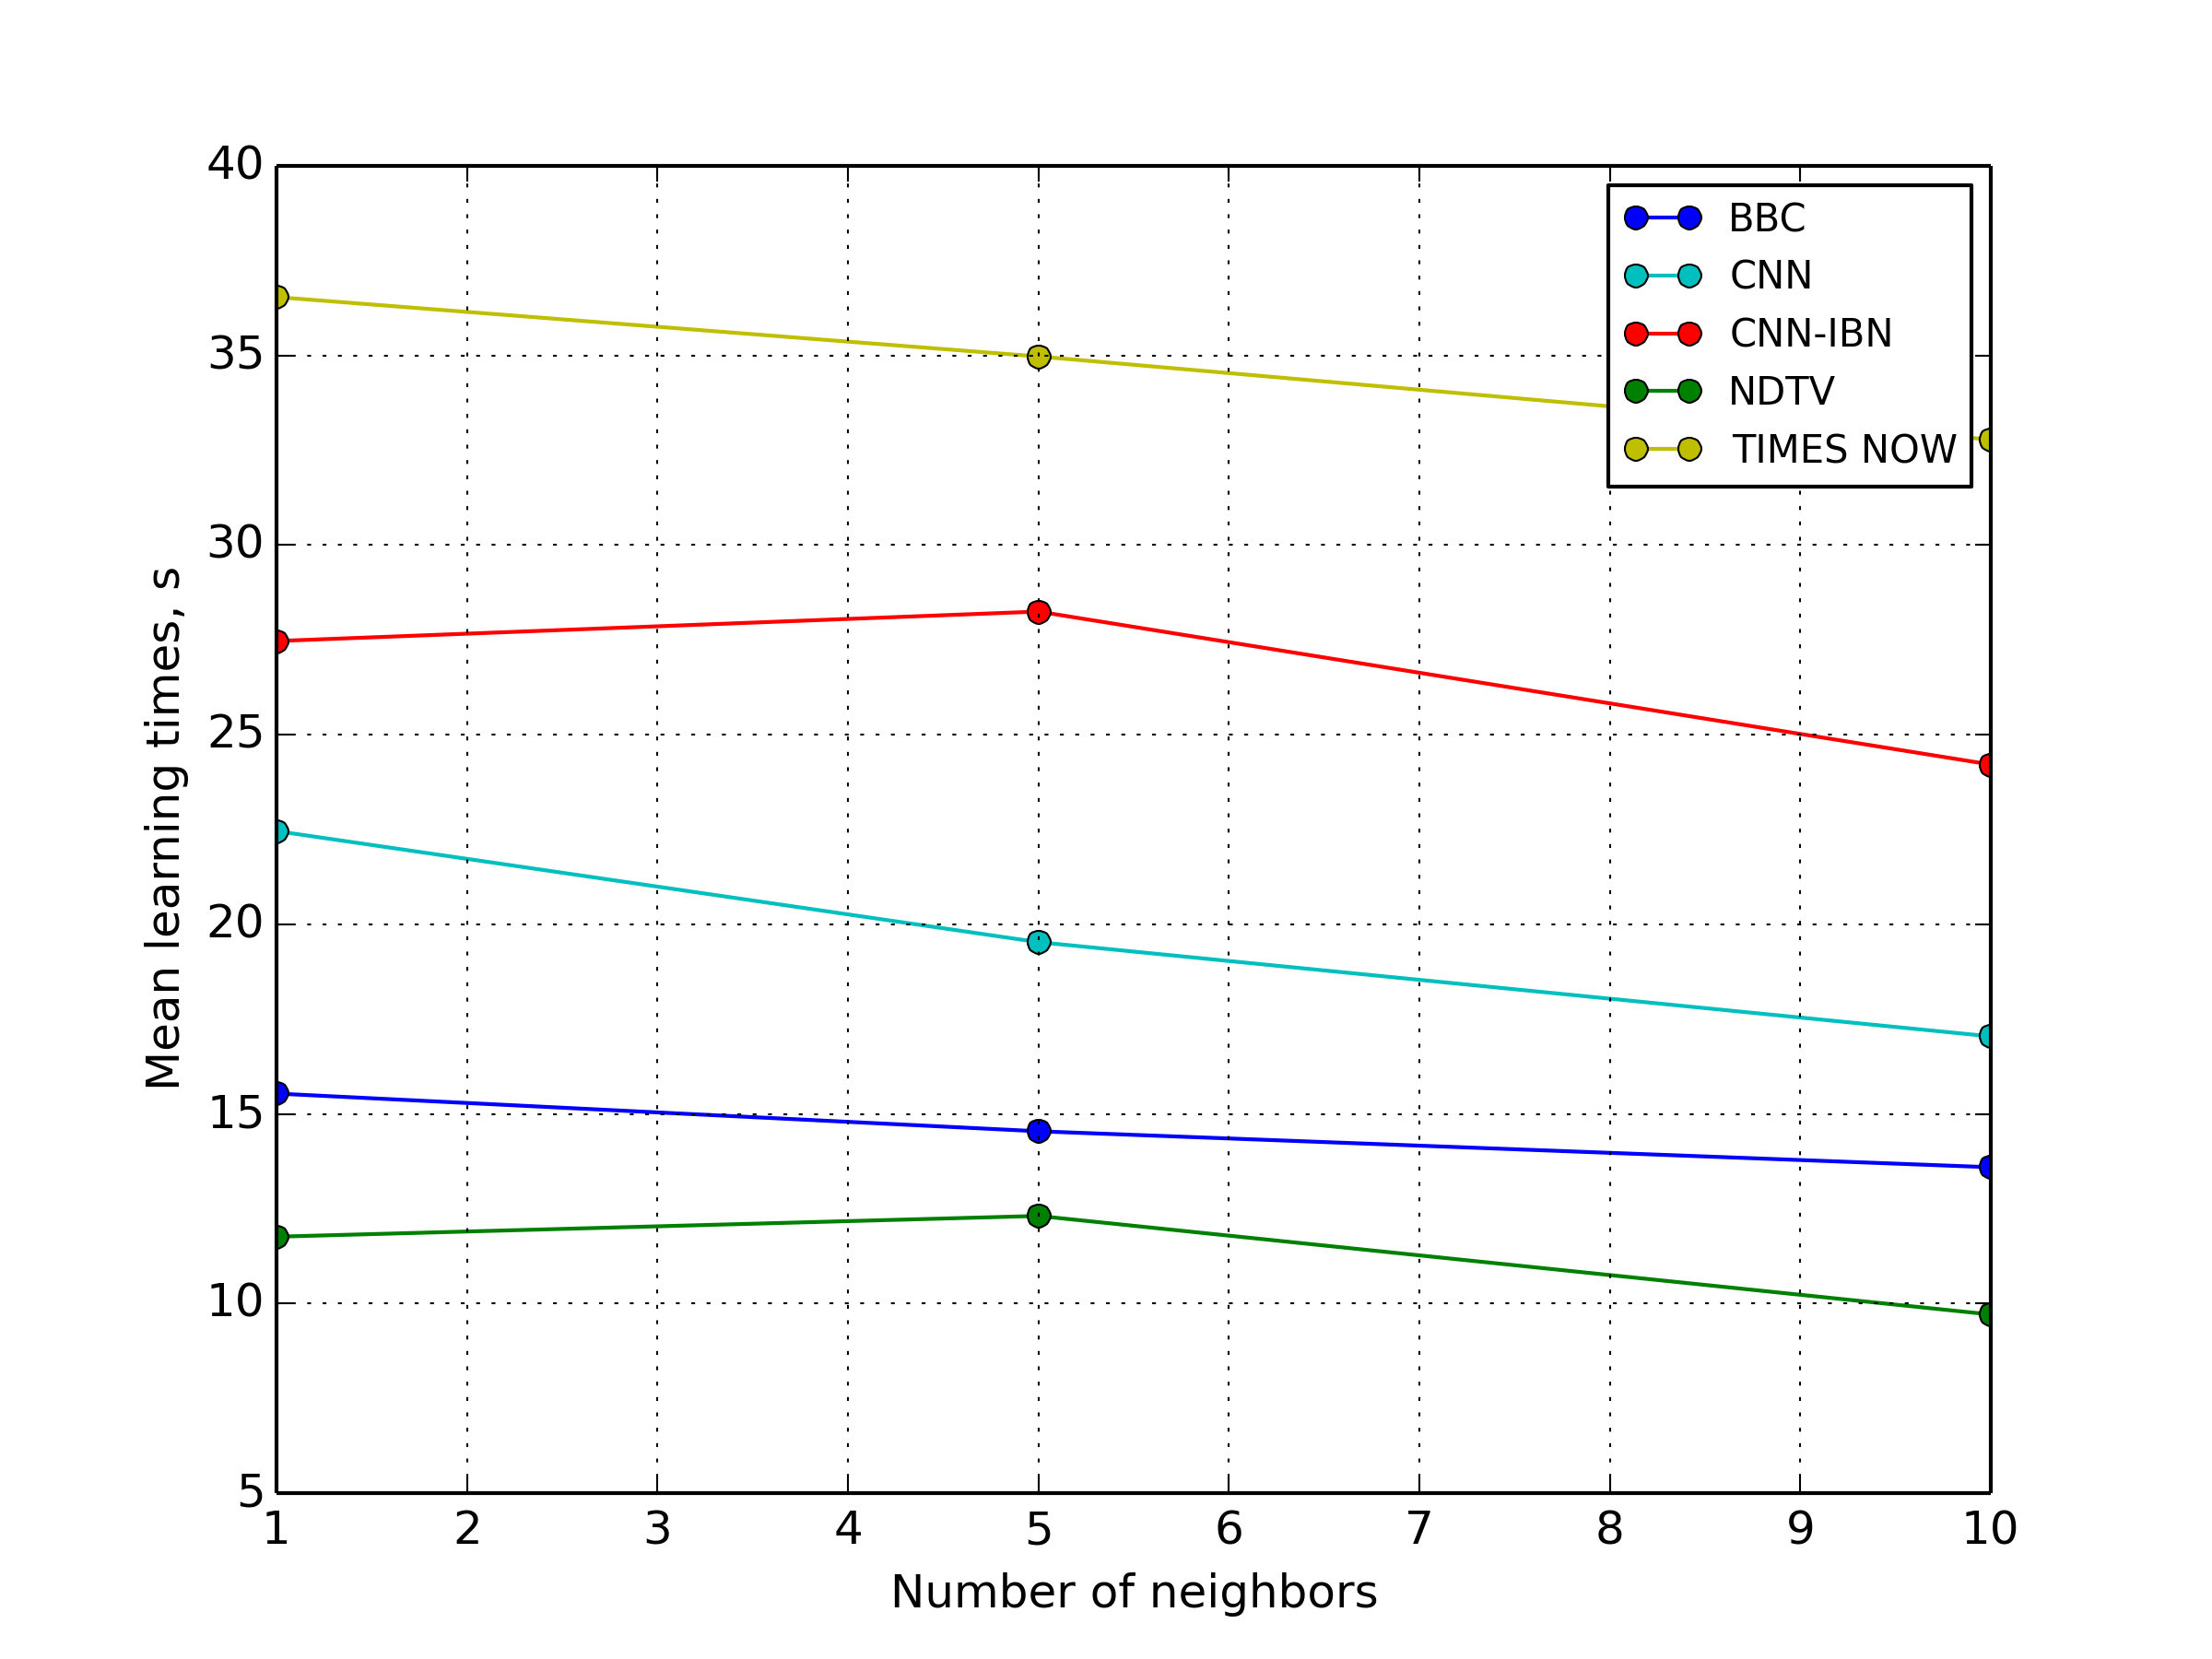
\includegraphics[width=\textwidth]{images/cnn-gradboostingTime.png}
		\caption{Время обучения.}
	\end{subfigure}
	\caption{Результаты применения CNN для GTB}\label{fig:cnn-gtb-results}
\end{figure}

В таблице~\ref{table:cnn-results} приведены результаты применения метода CNN при \(k=1\), как наиболее эффективного варианта. \(R\) и \(T_{PS}\) обозначены процент объектов выборки, оставленный методом CNN, и время работы CNN, соответственно. Как и в таблице~\ref{table:base-all}, \(Q\) означает качество классификации (в скобках указано абсолютное значение, на которое \(Q\) изменилось по сравнению с соответствующим значением в таблице~\ref{table:base-all}), и \(T_{tr}\) означает время обучения (в скобках указано во сколько раз время обучения после редукции больше времени обучения на всей выборке).

Из таблицы~\ref{table:cnn-results} видно, что несмотря на то, что \(k=1\) --- наилучший параметр из опробованных, метод CNN сильно портит качество классификации базовых методов. Объём выборки сокращается в 2--3 раза, и это приводит к ощутимому ускорению <<тяжёлых>> базовых методов --- SVM (ускорение от 4 до 10 раз) и градиентного бустинга (ускорение примерно в 3 раза). На некоторых каналах потери качества классификации не выглядят катастрофическими (связки случайный лес+CNN-IBN, случайный лес+NDTV, градиентный бустинг+NDTV), а вместе с полученными в этих случаях ускорениями, можно считать, что данные пары получили пользу от отбора эталонов. Самым неудобным для CNN оказался канал BBC --- от него осталась почти половина объектов и качество классификации базовыми методами на нём пострадало больше всего.

\begin{table}[h!]
    \centering
    \begin{tabular}{|c||c||c|c|}
		\cline{2-4}
		\multicolumn{1}{c||}{} & Сжатие \(T\) & \(k\)NN & LDA \\
		\hline \hline
		\input{cnn-table1.txt}
	\end{tabular}
	\newline \vspace*{0.5cm} \newline
	\centering
	\begin{tabular}{|c||c|c|c|}
		\cline{2-4}
		\multicolumn{1}{c||}{} & SVM & Random forest & GTB \\
		\hline \hline
		\input{cnn-table2.txt}
    \end{tabular}
    \caption{Сводная таблица результатов метода CNN и базовых методов после применения CNN}
    \label{table:cnn-results}
\end{table}

\subsection{Fast condensed nearest neighbor}
Метод FCNN \cite{angiulli} был предложен с целью исправить некоторые недостатки CNN и других методов, основанных на \(k\)NN: зависимость результирующего подмножества \(S\) от порядка элементов в обучающей выборке и низкая производительность и масштабируемость. Он, как и CNN, является методом сгущения.

FCNN работает следующим образом. Изначально \(S\) содержит точки, ближайшие к барицентрам классов (барицентр класса --- \(\mathbf{x}_C=|C|^{-1}\sum_{c\in C}\mathbf{x}_c\), где \(C\) --- множество индексов объектов, принадлежащих одному классу). Затем, множество \(T\setminus S\) разбивается на \(|S|\) непересекающихся классов \(Vor(p, S, T)\) (так называемые Voronoi cells), в каждом из которых находятся объекты, для которых ближайшим соседом является один и тот же объект \(p\in S\). Затем все объекты из \(T\setminus S\) классифицируются методом ближайшего соседа с обучающей выборкой \(S\), и в каждом \(Vor(p, S, T)\) выбираются неверно классифицированные объекты, которые составляют множества \(Voren(p, S, T)\) (Voronoi enemies). После этого для каждого такого \(p\in S\), что \(Voren(p, S, T)\neq\varnothing\) выбирается ближайший к \(p\) объект из \(Voren(p, S, T)\) и добавляется в \(S\). На каждой следующей итерации процедура повторяется для нового \(S\). Алгоритм останавливается, когда на последней итерации в \(S\) не было добавлено ни одного элемента.

FCNN может быть расширен на число ближайших соседей, отличных от 1, аналогично CNN: при классификации объектов в \(T\setminus S\) нужно использовать метод \(k\)NN. В \cite{angiulli} приведено доказательство того, что он строит согласованное подмножество \(S\), одинаковое для любого упорядочивания обучающей выборки.

\subsubsection*{Результаты применения FCNN}
Аналогично CNN, с FCNN были проведены эксперименты для \(k\in\{1,5,10\}\). Доли отобранных объектов и времена работы для каждого из каналов приведены на рис.~\ref{fig:fcnn-stats}. В данном случае очевидно полное преимущество \(k=1\) над другими значениями параметра в смысле результатов FCNN.
\begin{figure}[h!]
    \centering
	\begin{subfigure}{0.45\textwidth}
		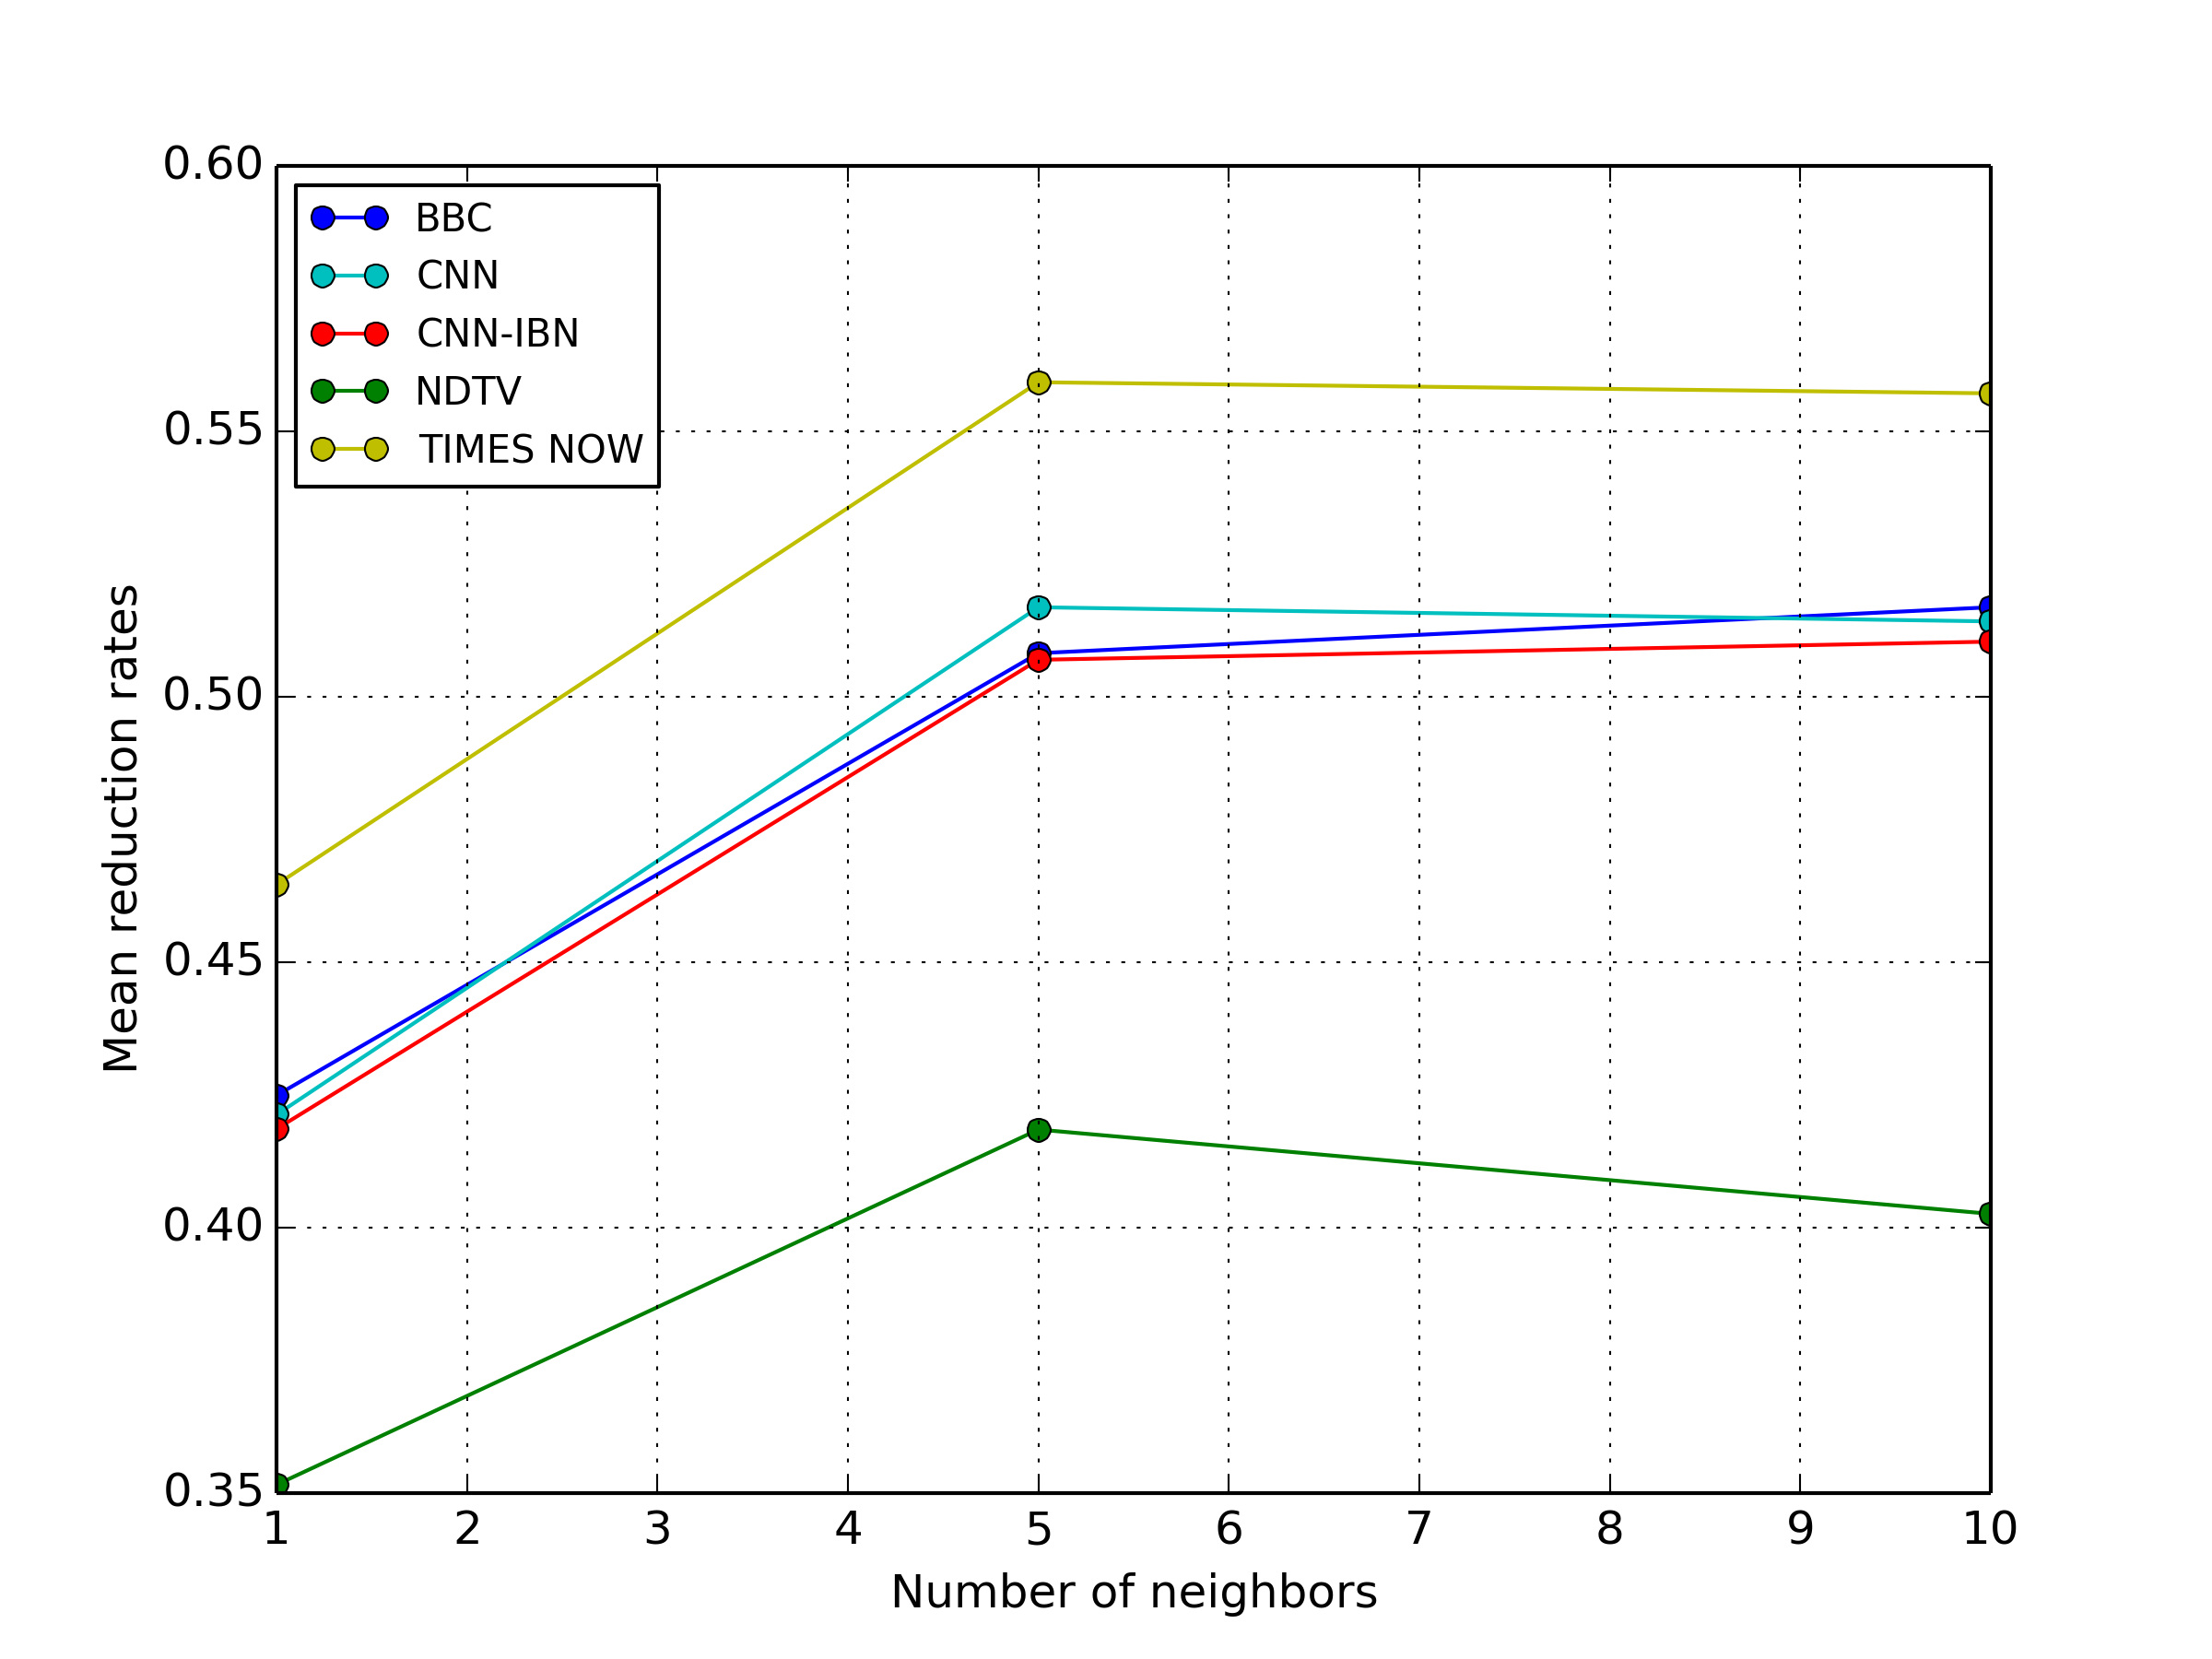
\includegraphics[width=\textwidth]{images/fcnn-stats.png}
		\caption{Доля отобранных объектов.}
	\end{subfigure}
	\begin{subfigure}{0.45\textwidth}
		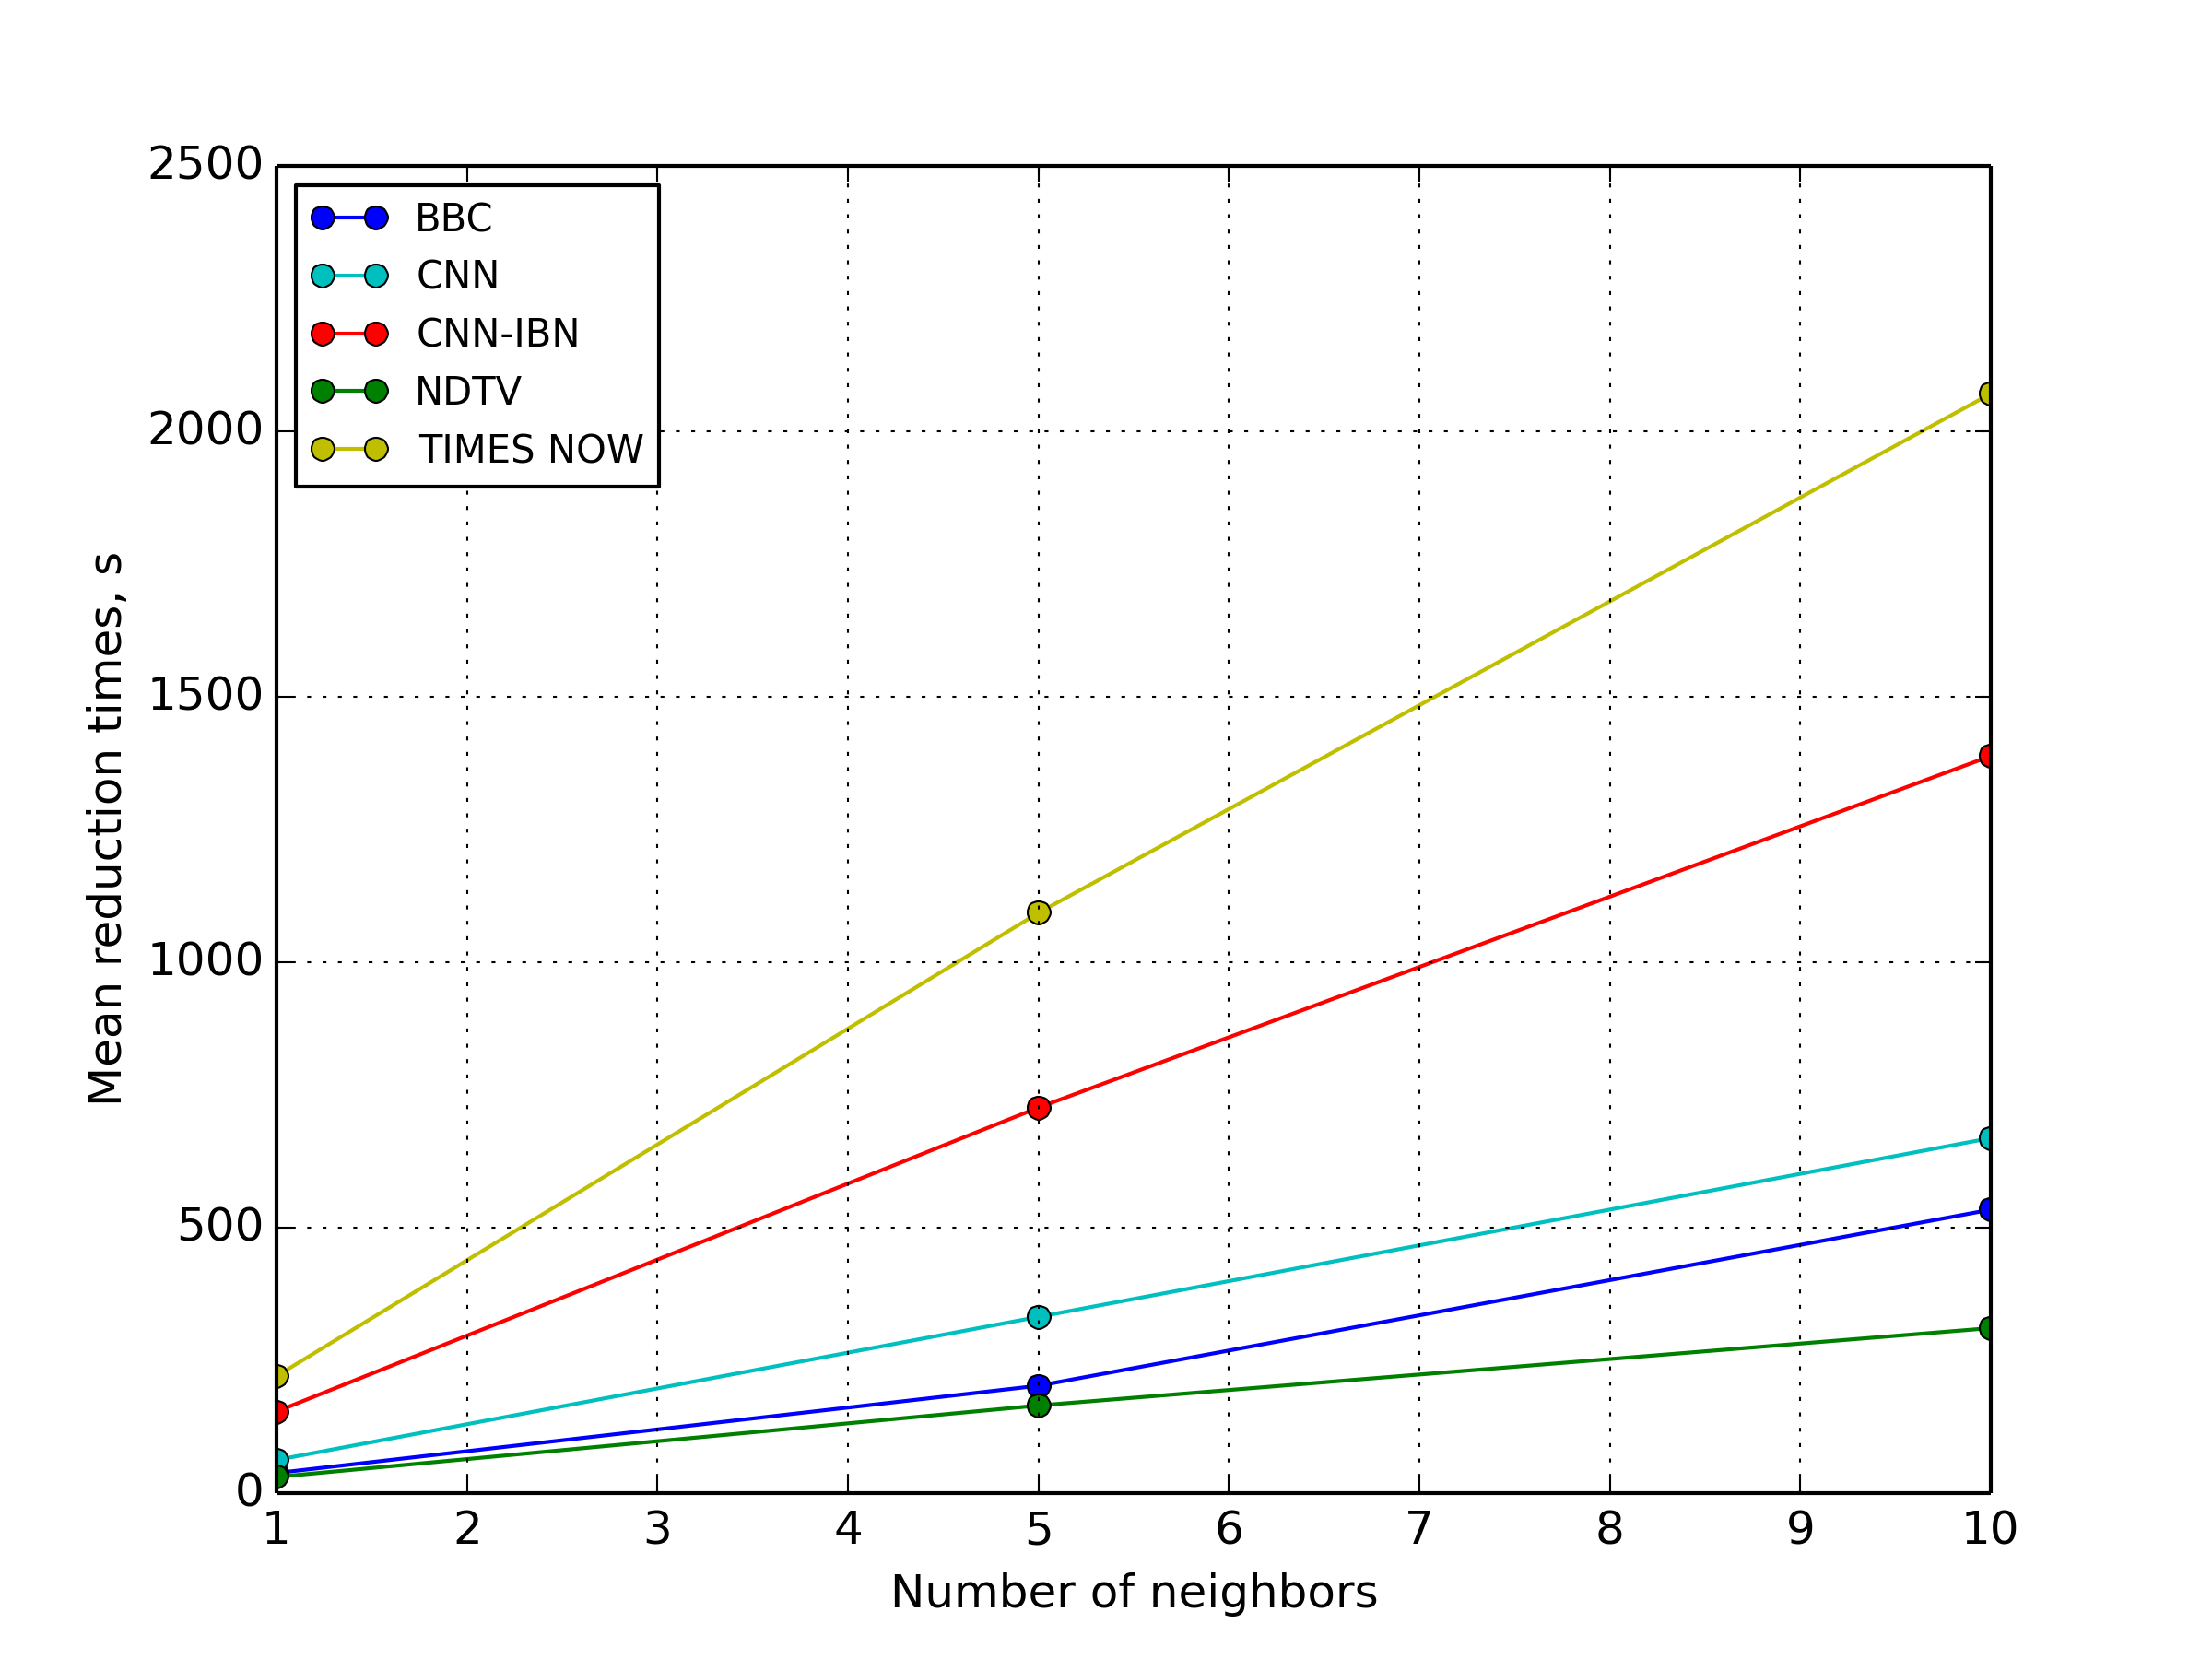
\includegraphics[width=\textwidth]{images/fcnn-TimeStats.png}
		\caption{Время, потраченное на отбор эталонов.}
	\end{subfigure}
	\caption{Результаты работы FCNN.}\label{fig:fcnn-stats}
\end{figure}

На рис.~\ref{fig:fcnn-knn-results}--\ref{fig:fcnn-gtb-results} приведены результаты работы базовых методах на обучающих выборках, редуцированных с помощью FCNN. С этим методом ситуация получается противоположная CNN --- меньший \(k\) обеспечивает большую редукцию, но при этом базовые методы после редукции дают похожие качества классификации для всех \(k\). Одно из объяснений этому --- за счёт более сложной эвристики FCNN отбирает более качественные эталоны, что нивелирует разницу для базовых методов. С другой стороны, сама процедура FCNN оказывается более подвержена ошибкам классификации на границе классов для неединичных \(k\), поэтому она выполняет больше итераций.

\begin{figure}[h!]
    \centering
	\begin{subfigure}{0.45\textwidth}
		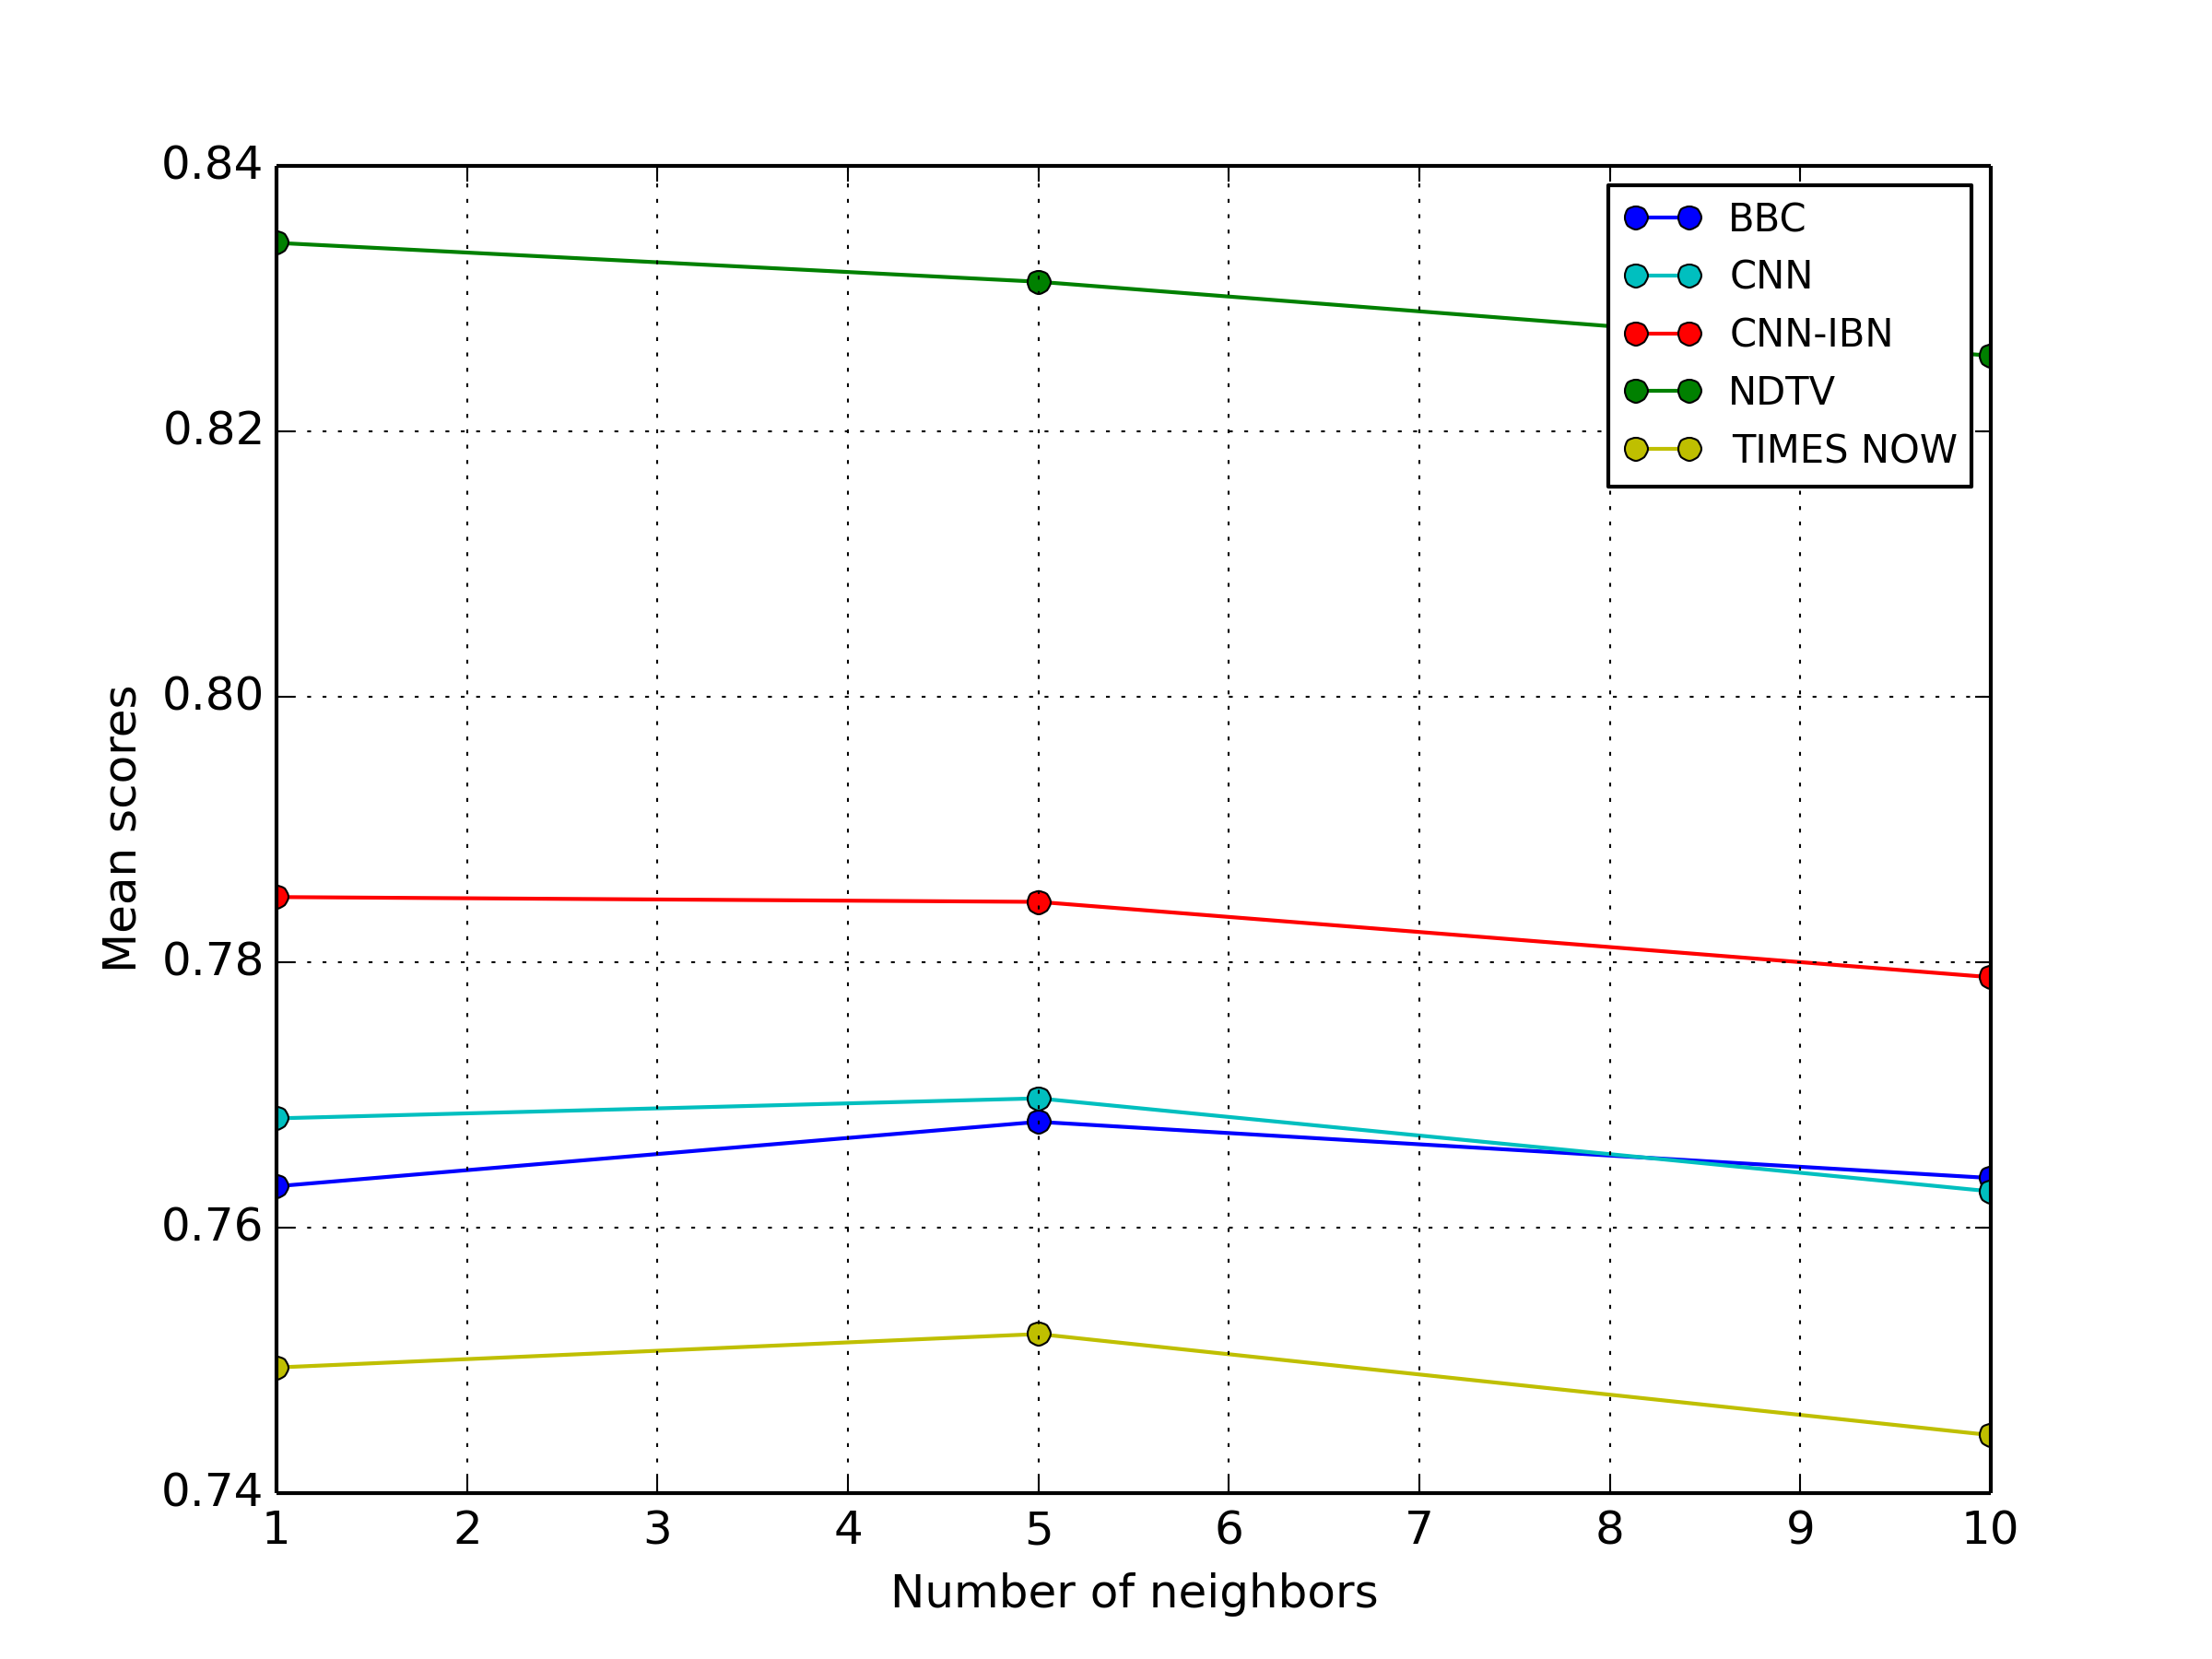
\includegraphics[width=\textwidth]{images/fcnn-KNN.png}
		\caption{Качество классификации.}
	\end{subfigure}
	\begin{subfigure}{0.45\textwidth}
		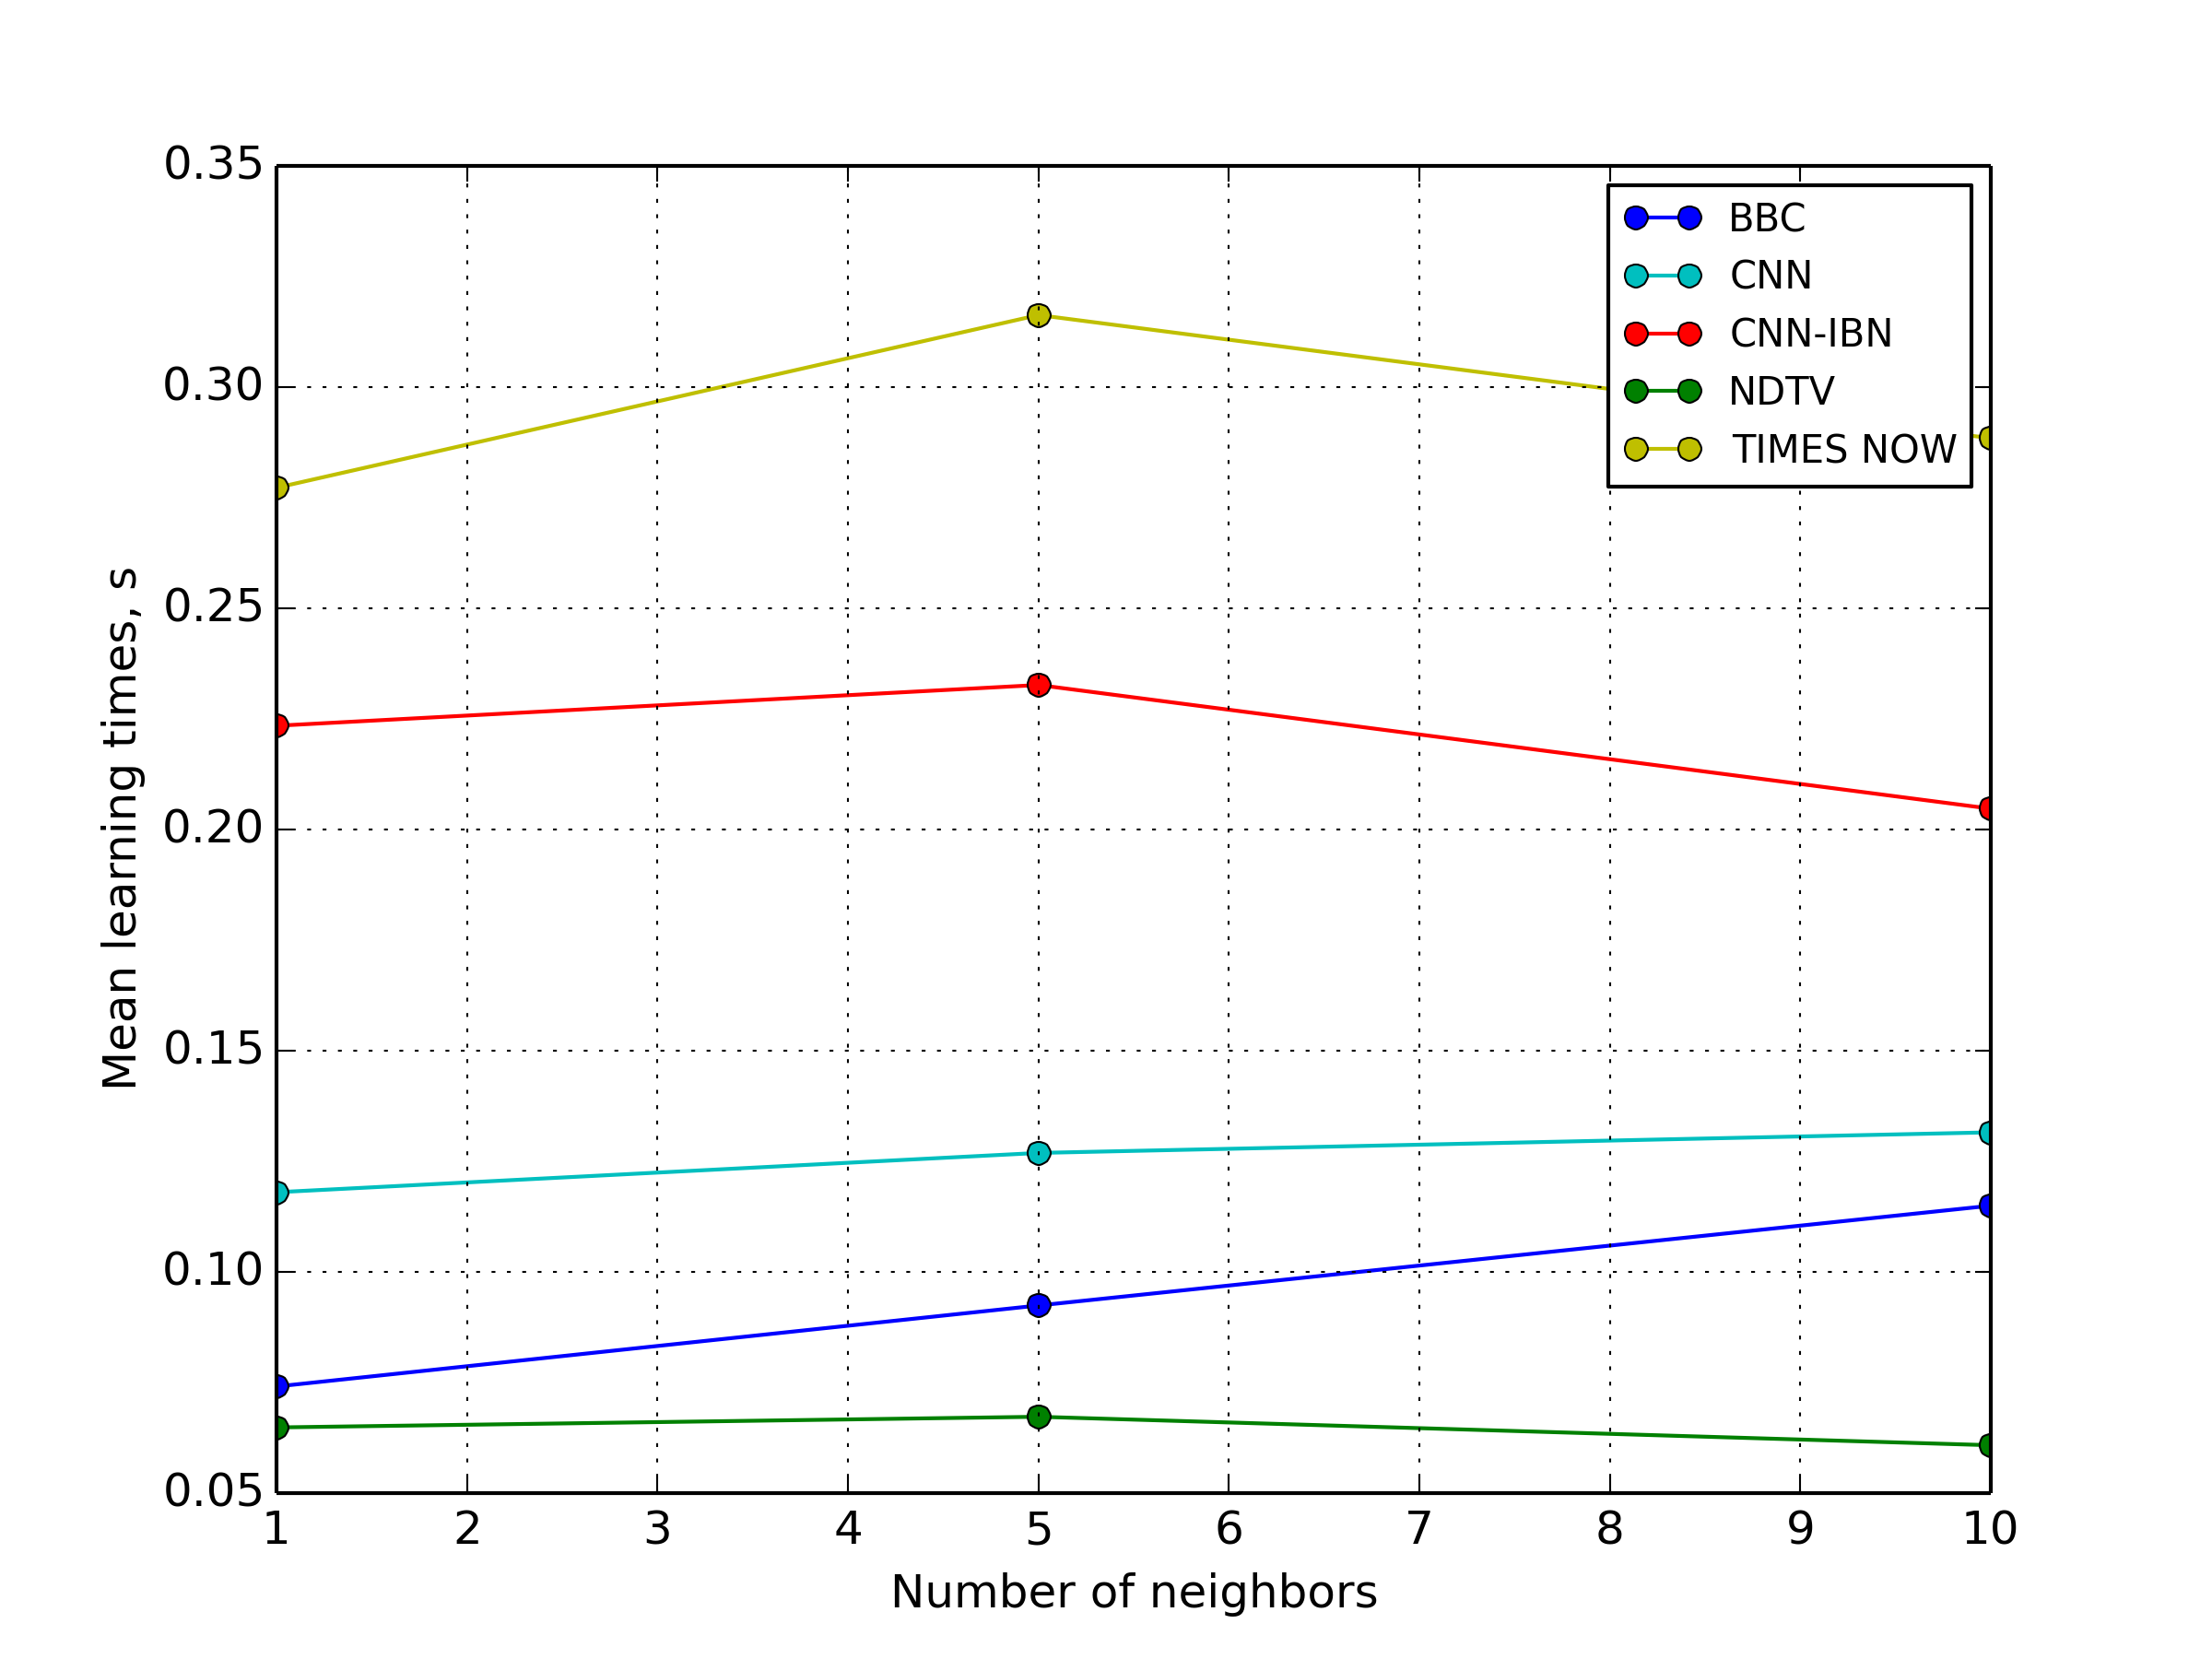
\includegraphics[width=\textwidth]{images/fcnn-KNNTime.png}
		\caption{Время обучения.}
	\end{subfigure}
	\caption{Результаты применения FCNN для 15-NN.}\label{fig:fcnn-knn-results}
\end{figure}

\begin{figure}[h!]
	\centering
	\begin{subfigure}{0.45\textwidth}
		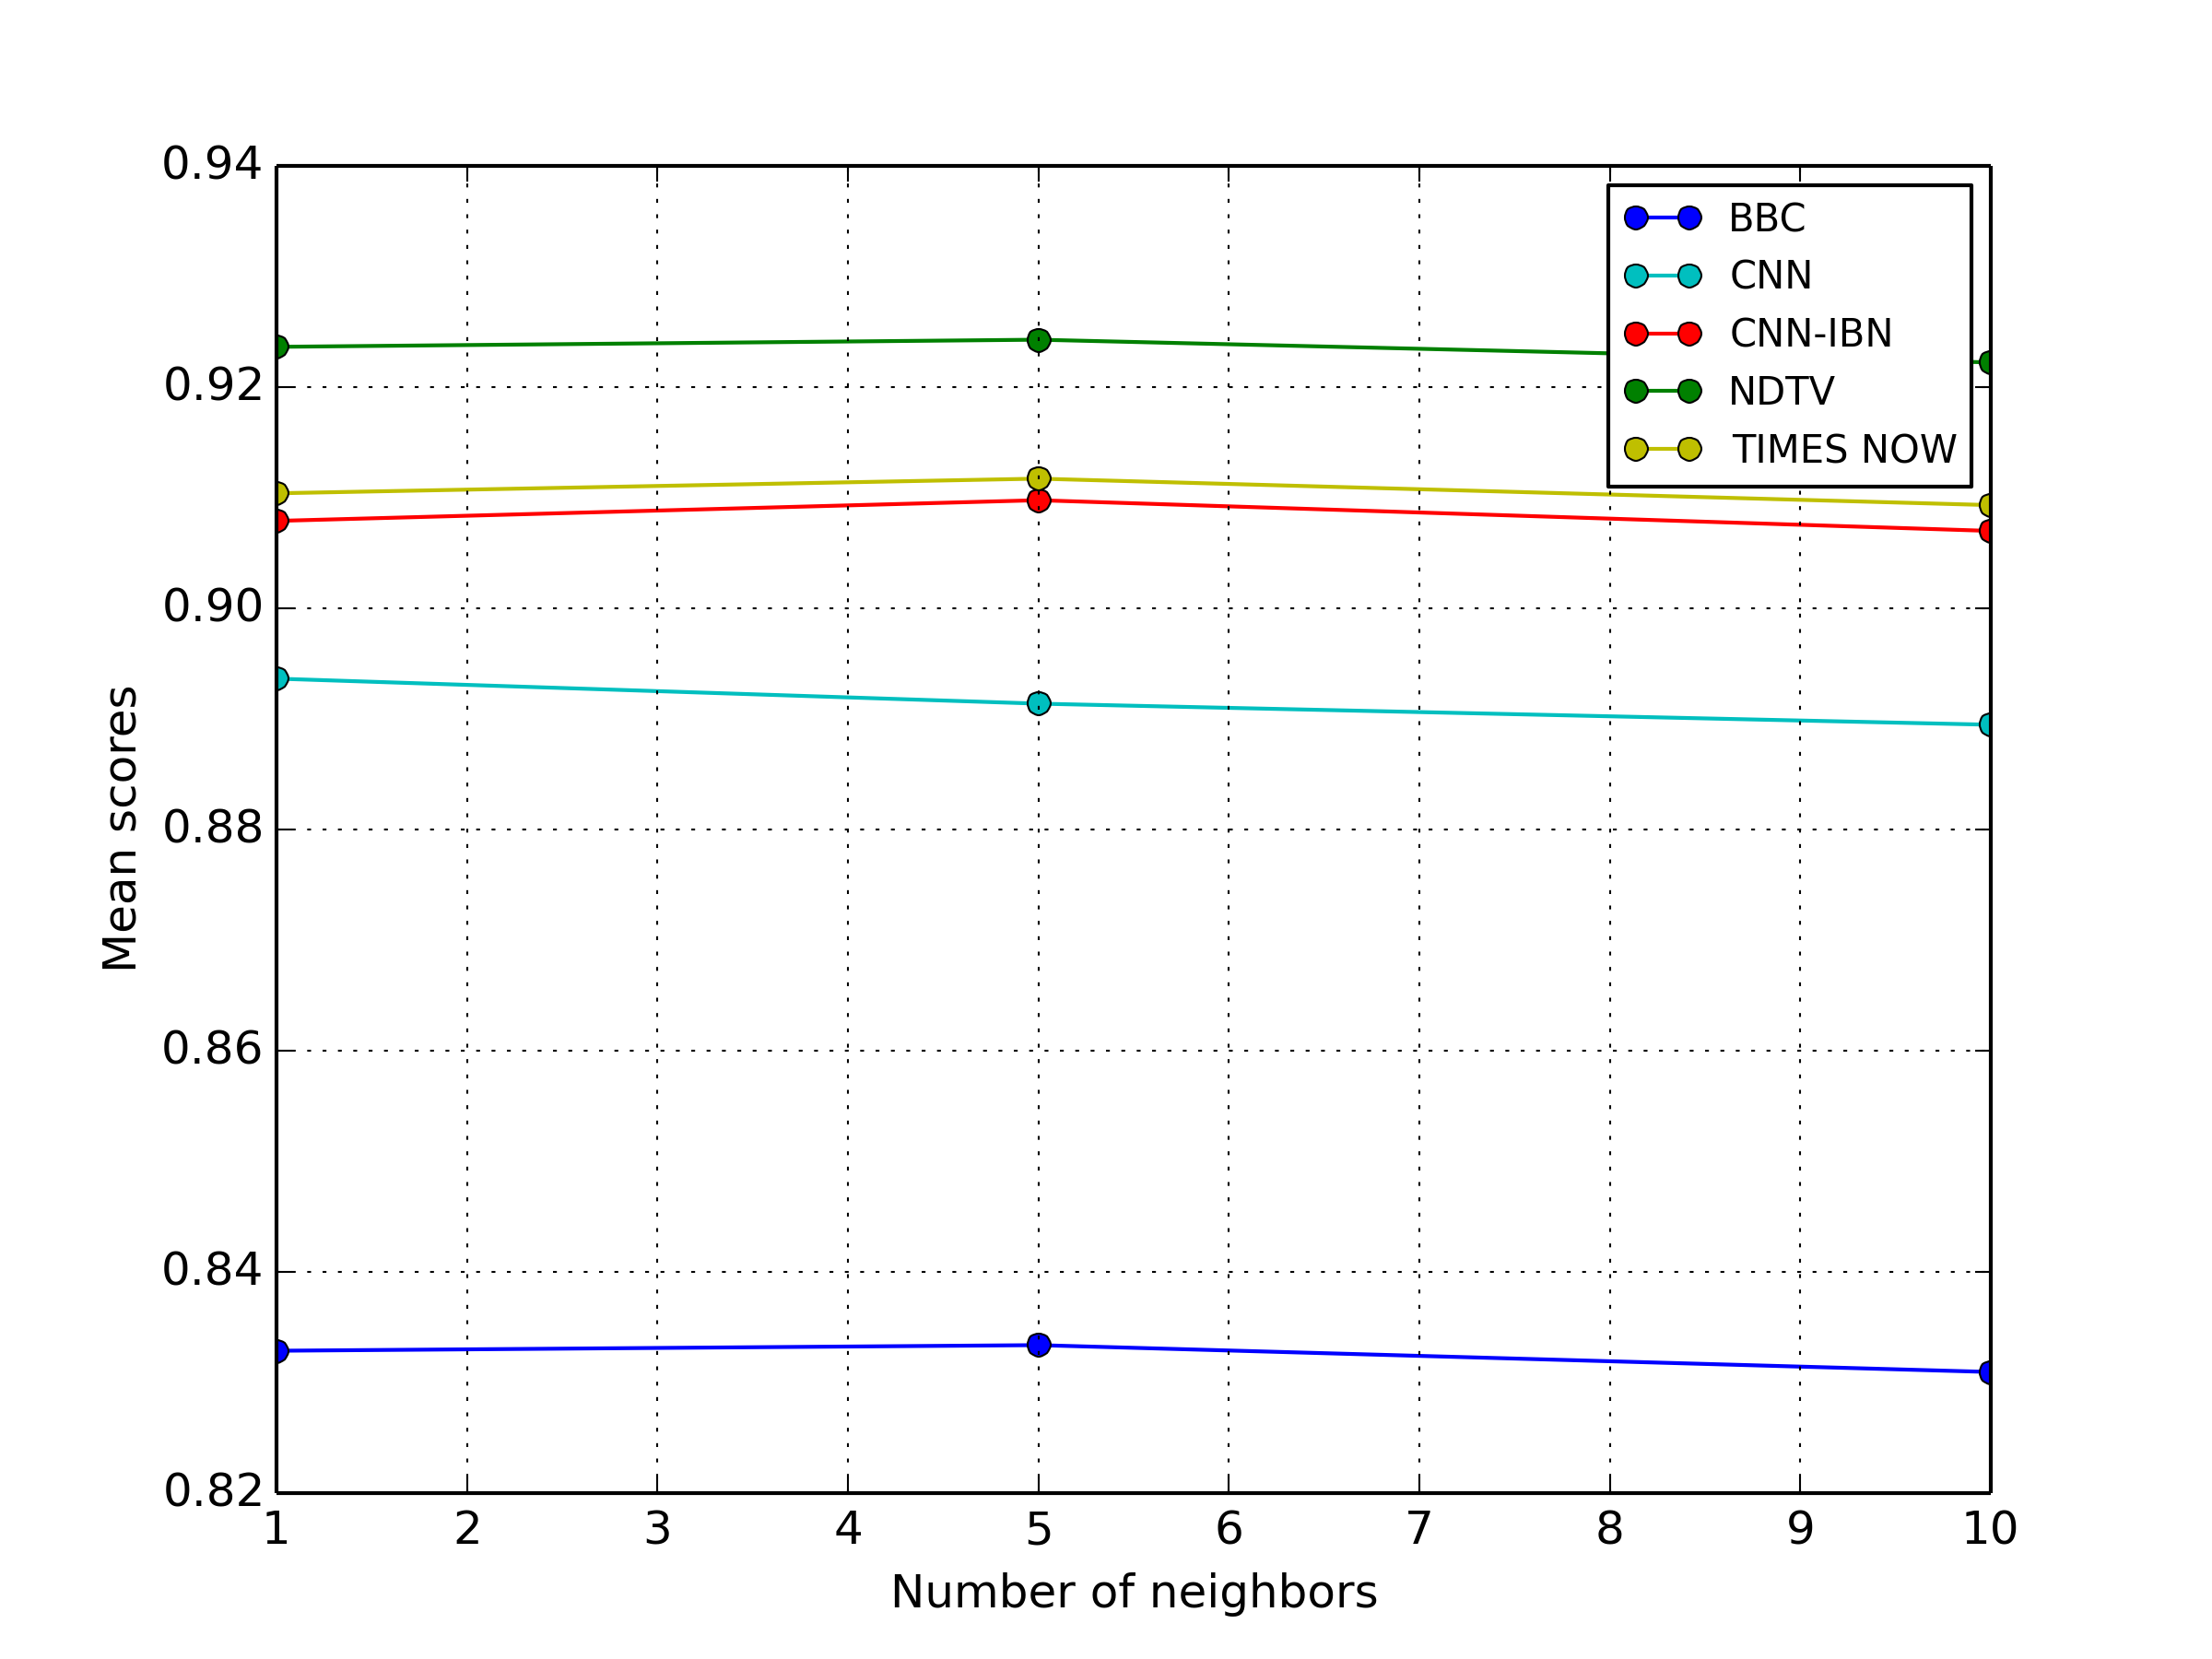
\includegraphics[width=\textwidth]{images/fcnn-LDA.png}
		\caption{Качество классификации.}
	\end{subfigure}
	\begin{subfigure}{0.45\textwidth}
		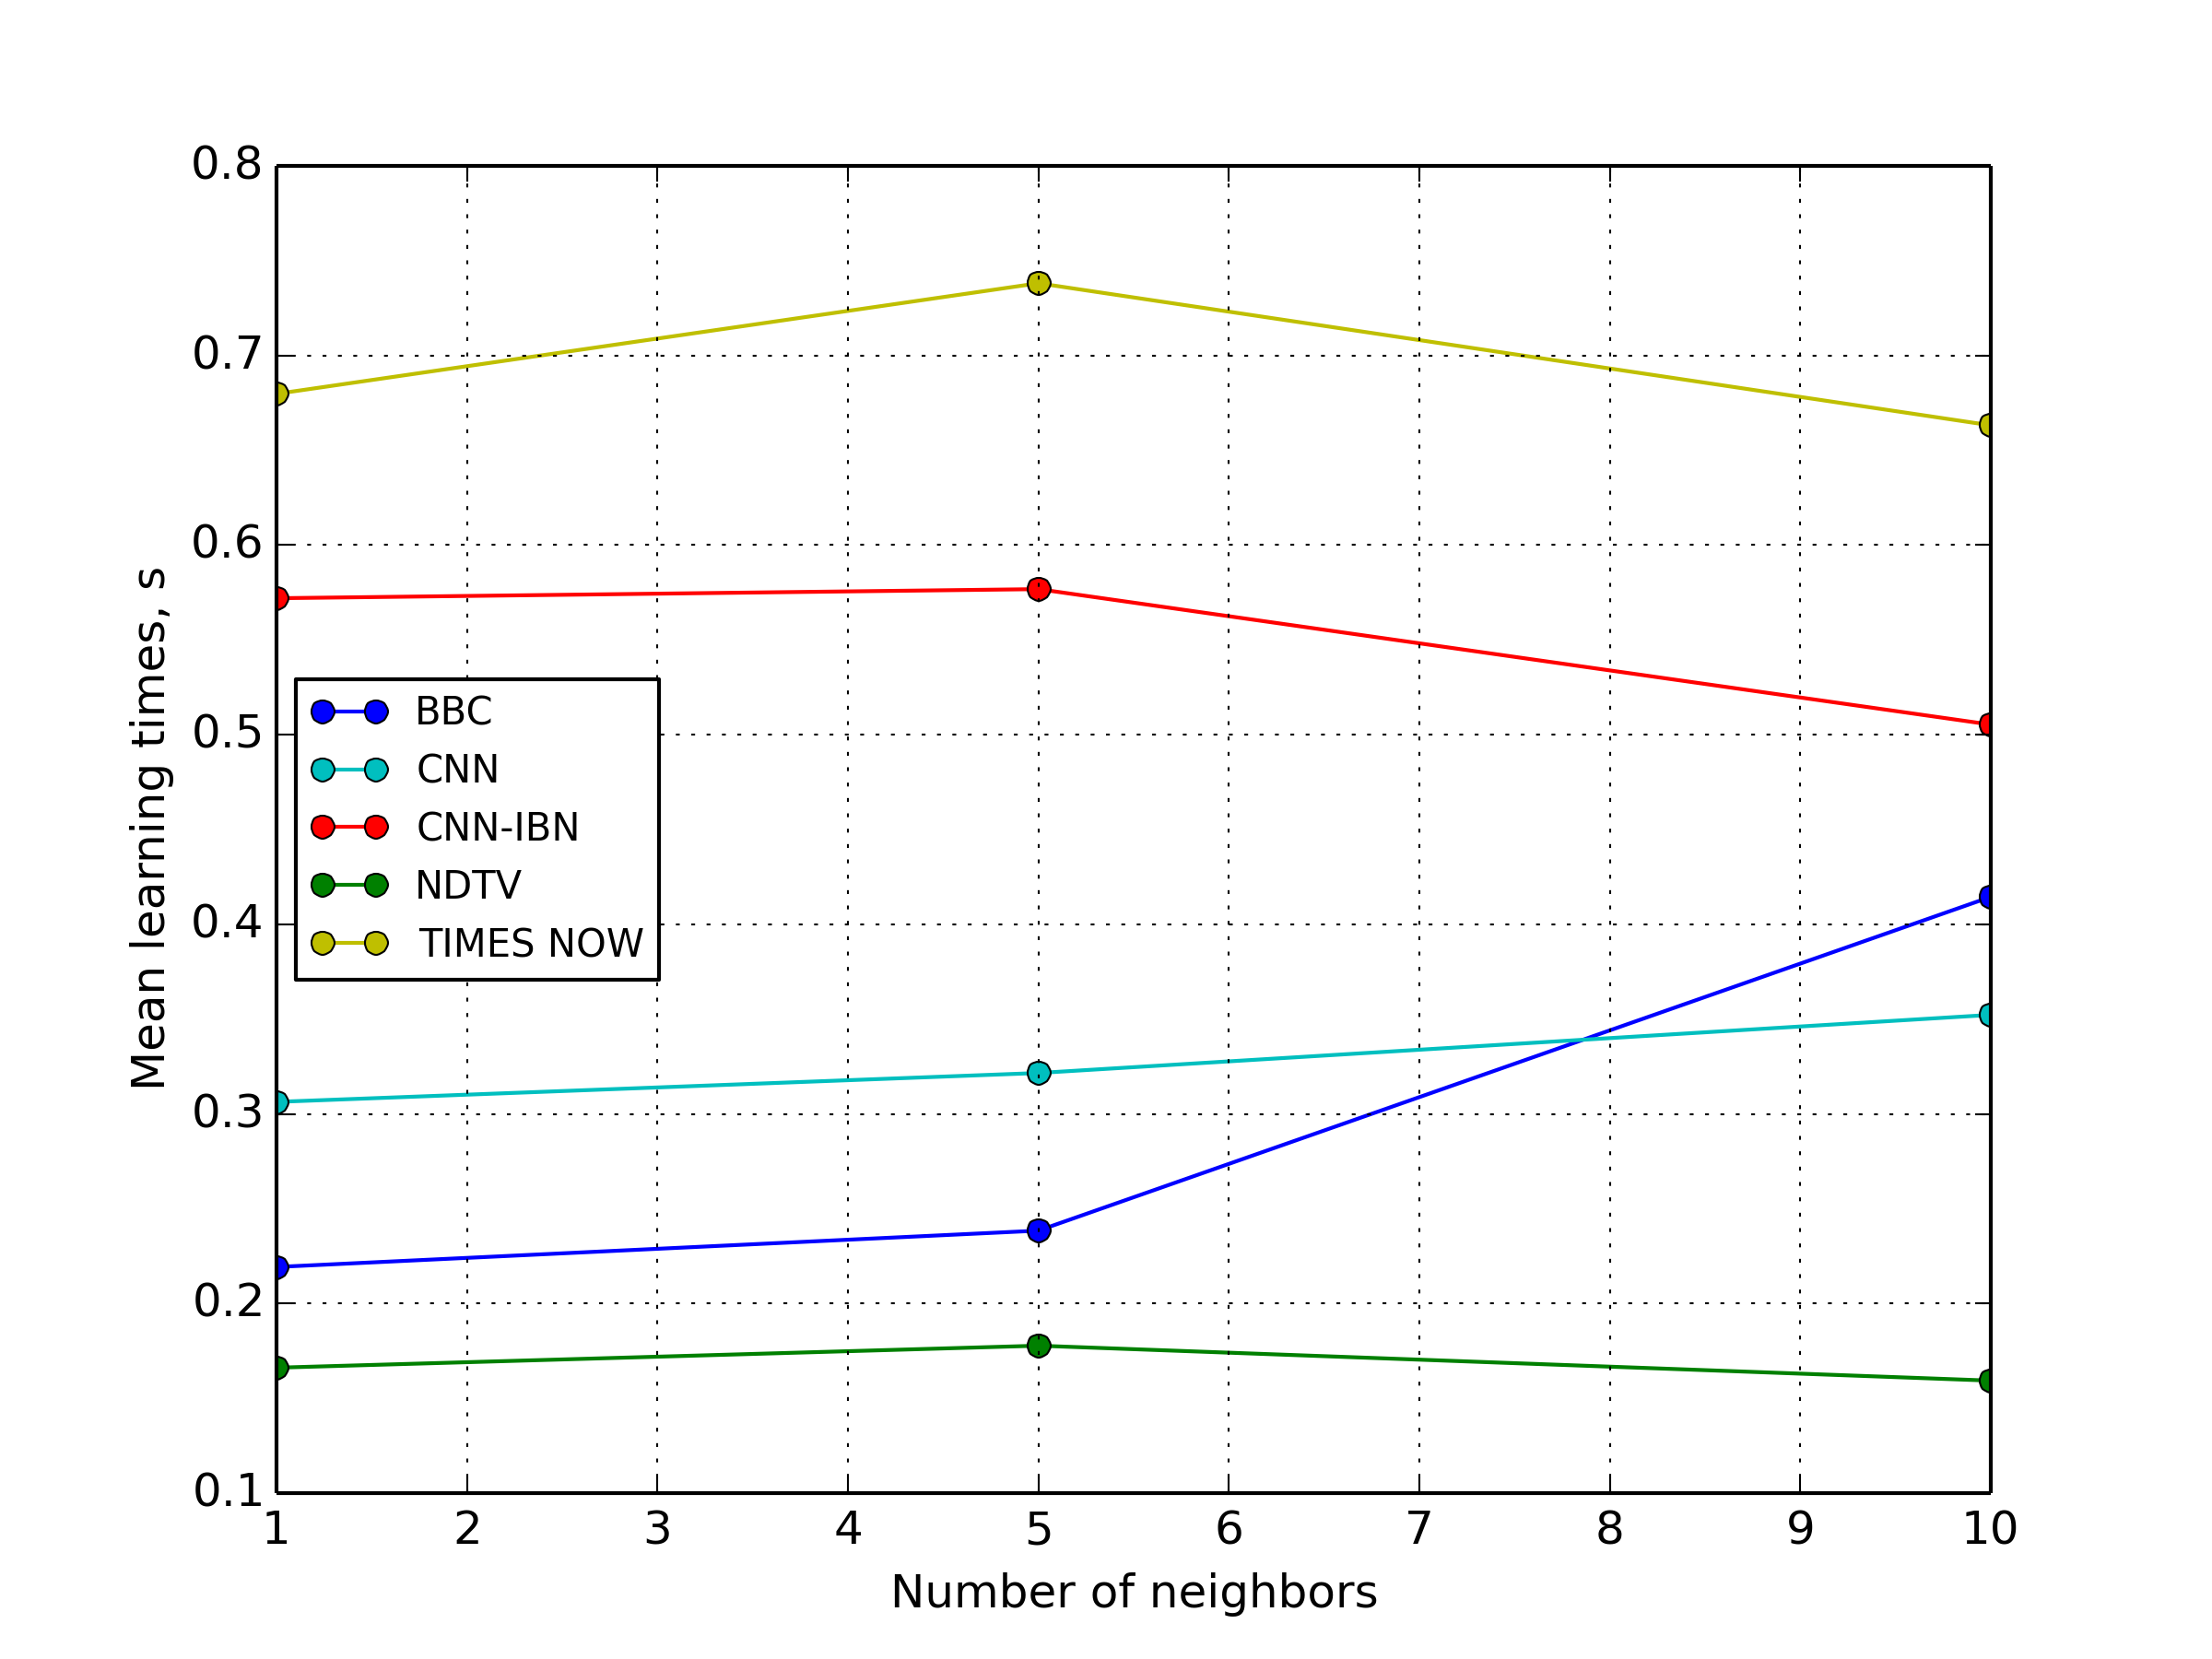
\includegraphics[width=\textwidth]{images/fcnn-LDATime.png}
		\caption{Время обучения.}
	\end{subfigure}
	\caption{Результаты применения FCNN для LDA.}\label{fig:fcnn-lda-results}
\end{figure}

\begin{figure}[h!]
	\centering
	\begin{subfigure}{0.45\textwidth}
		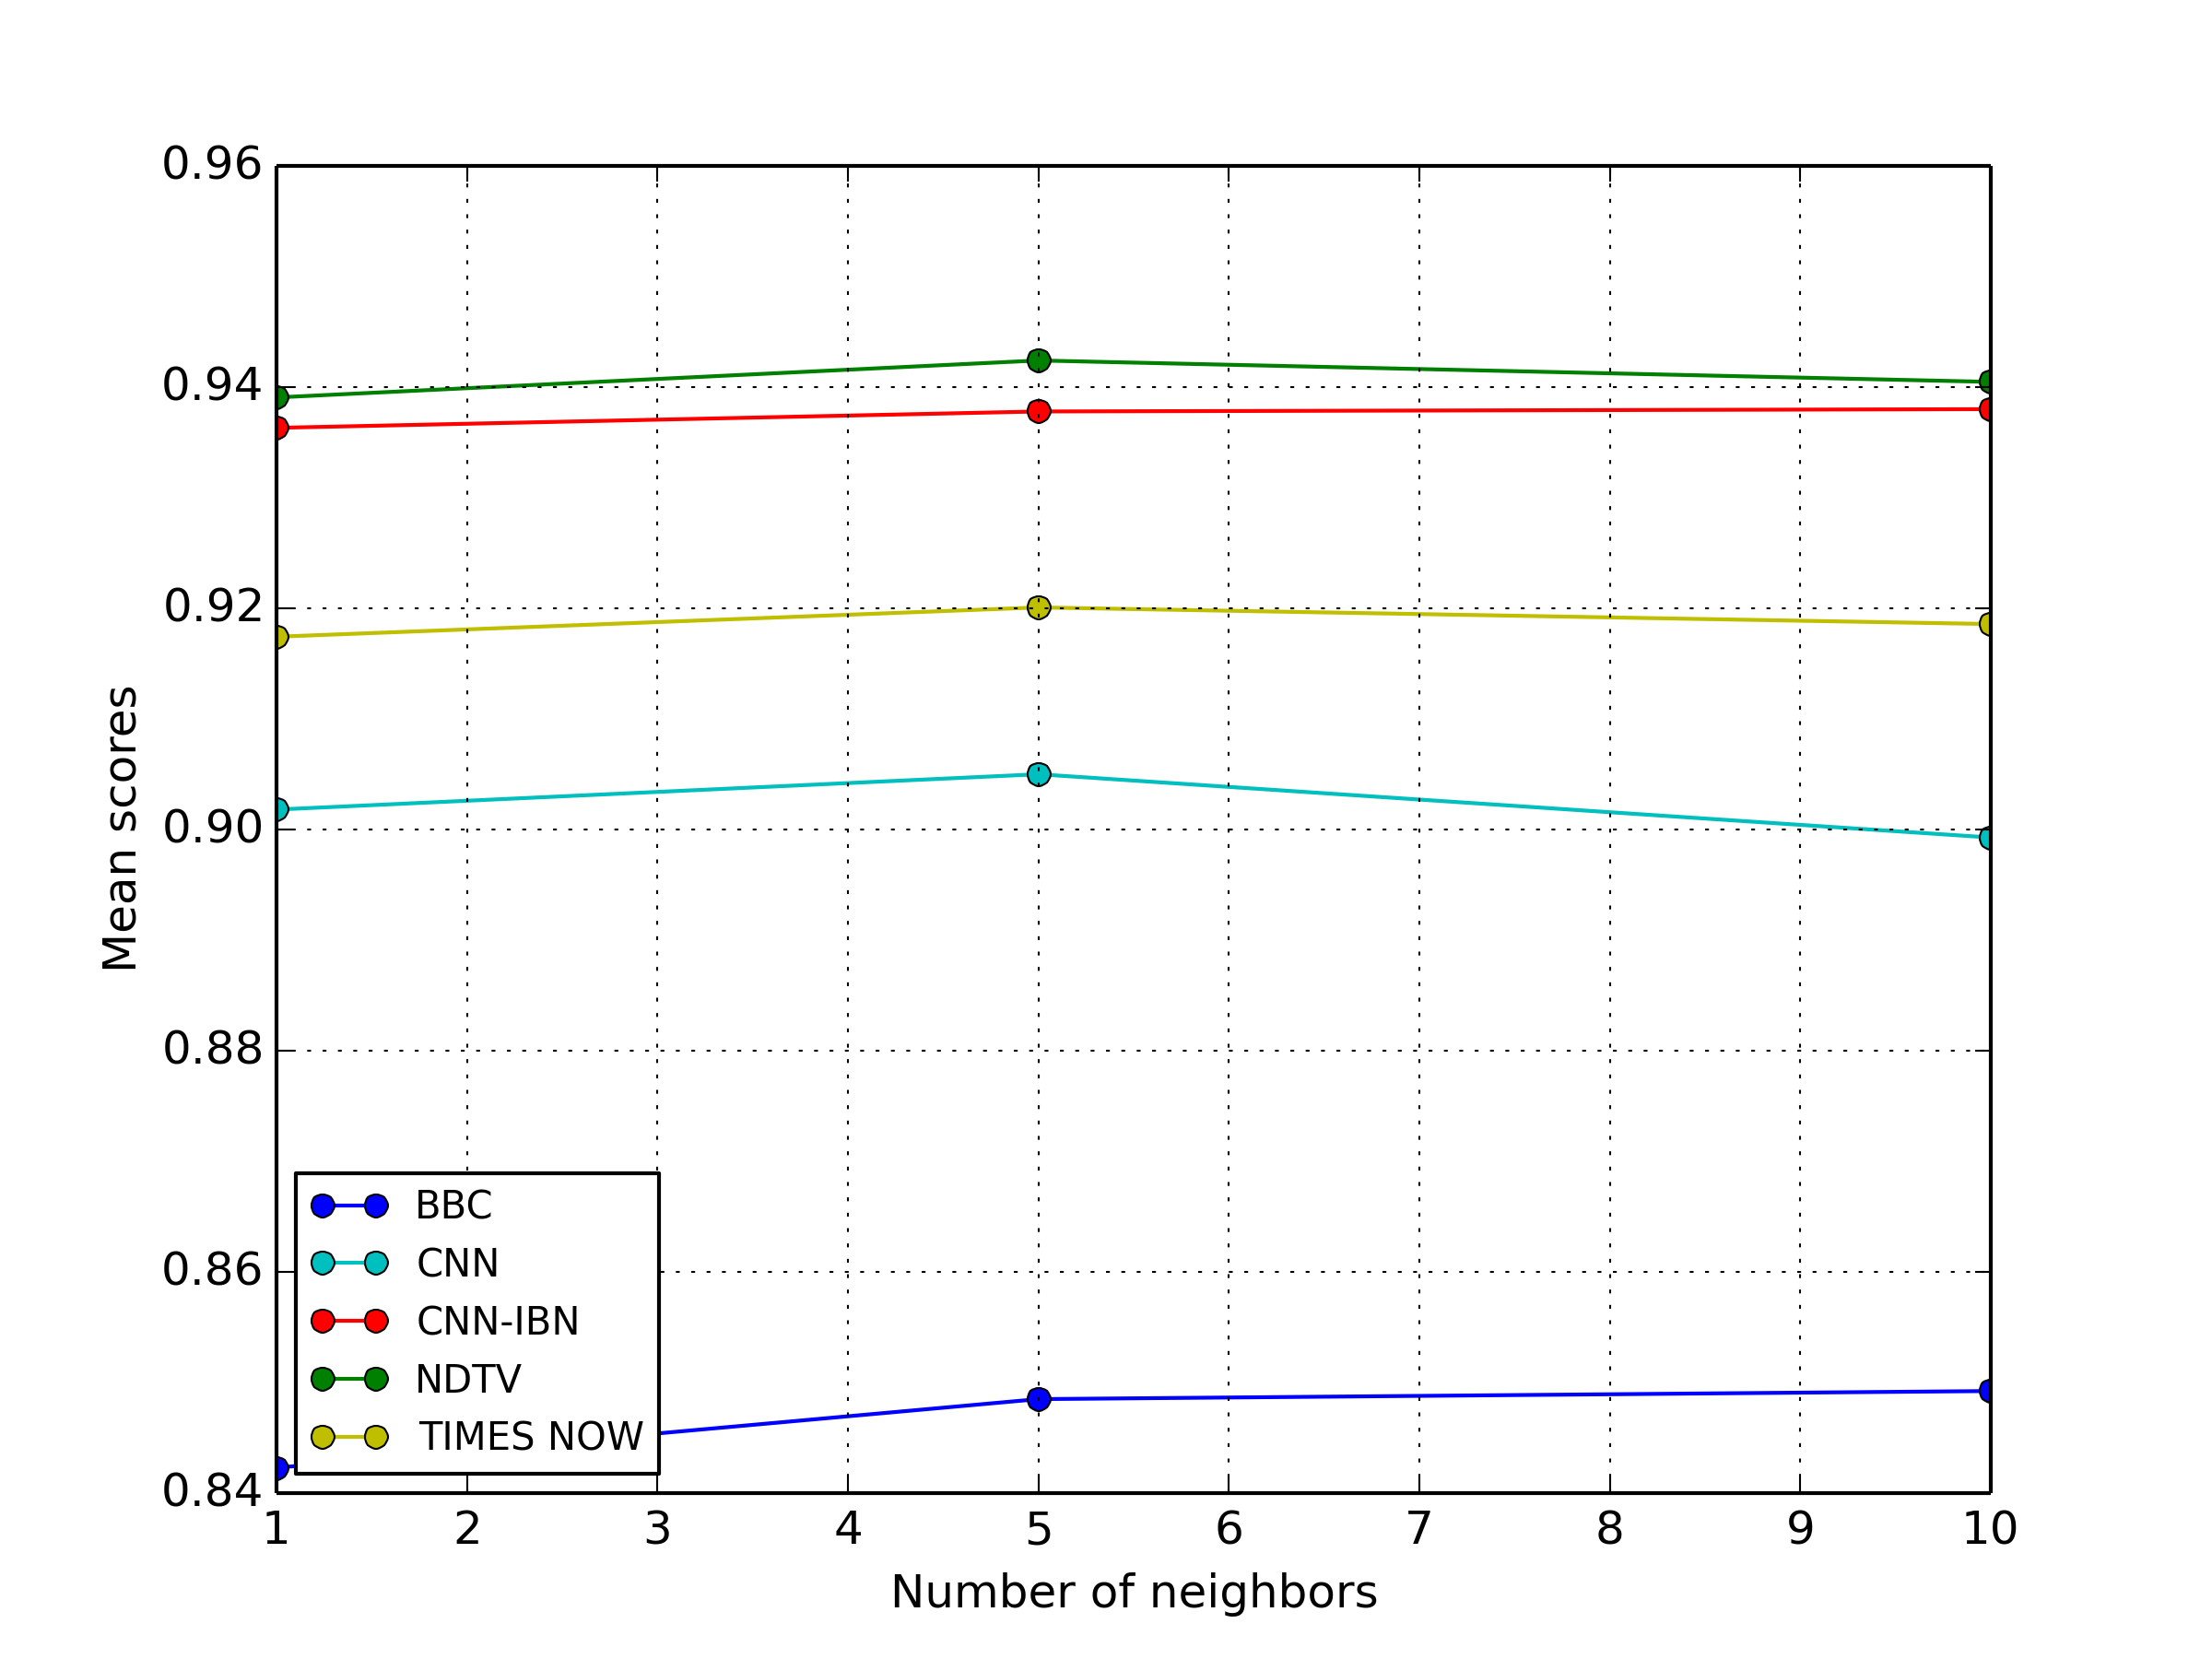
\includegraphics[width=\textwidth]{images/fcnn-SVM.png}
		\caption{Качество классификации.}
	\end{subfigure}
	\begin{subfigure}{0.45\textwidth}
		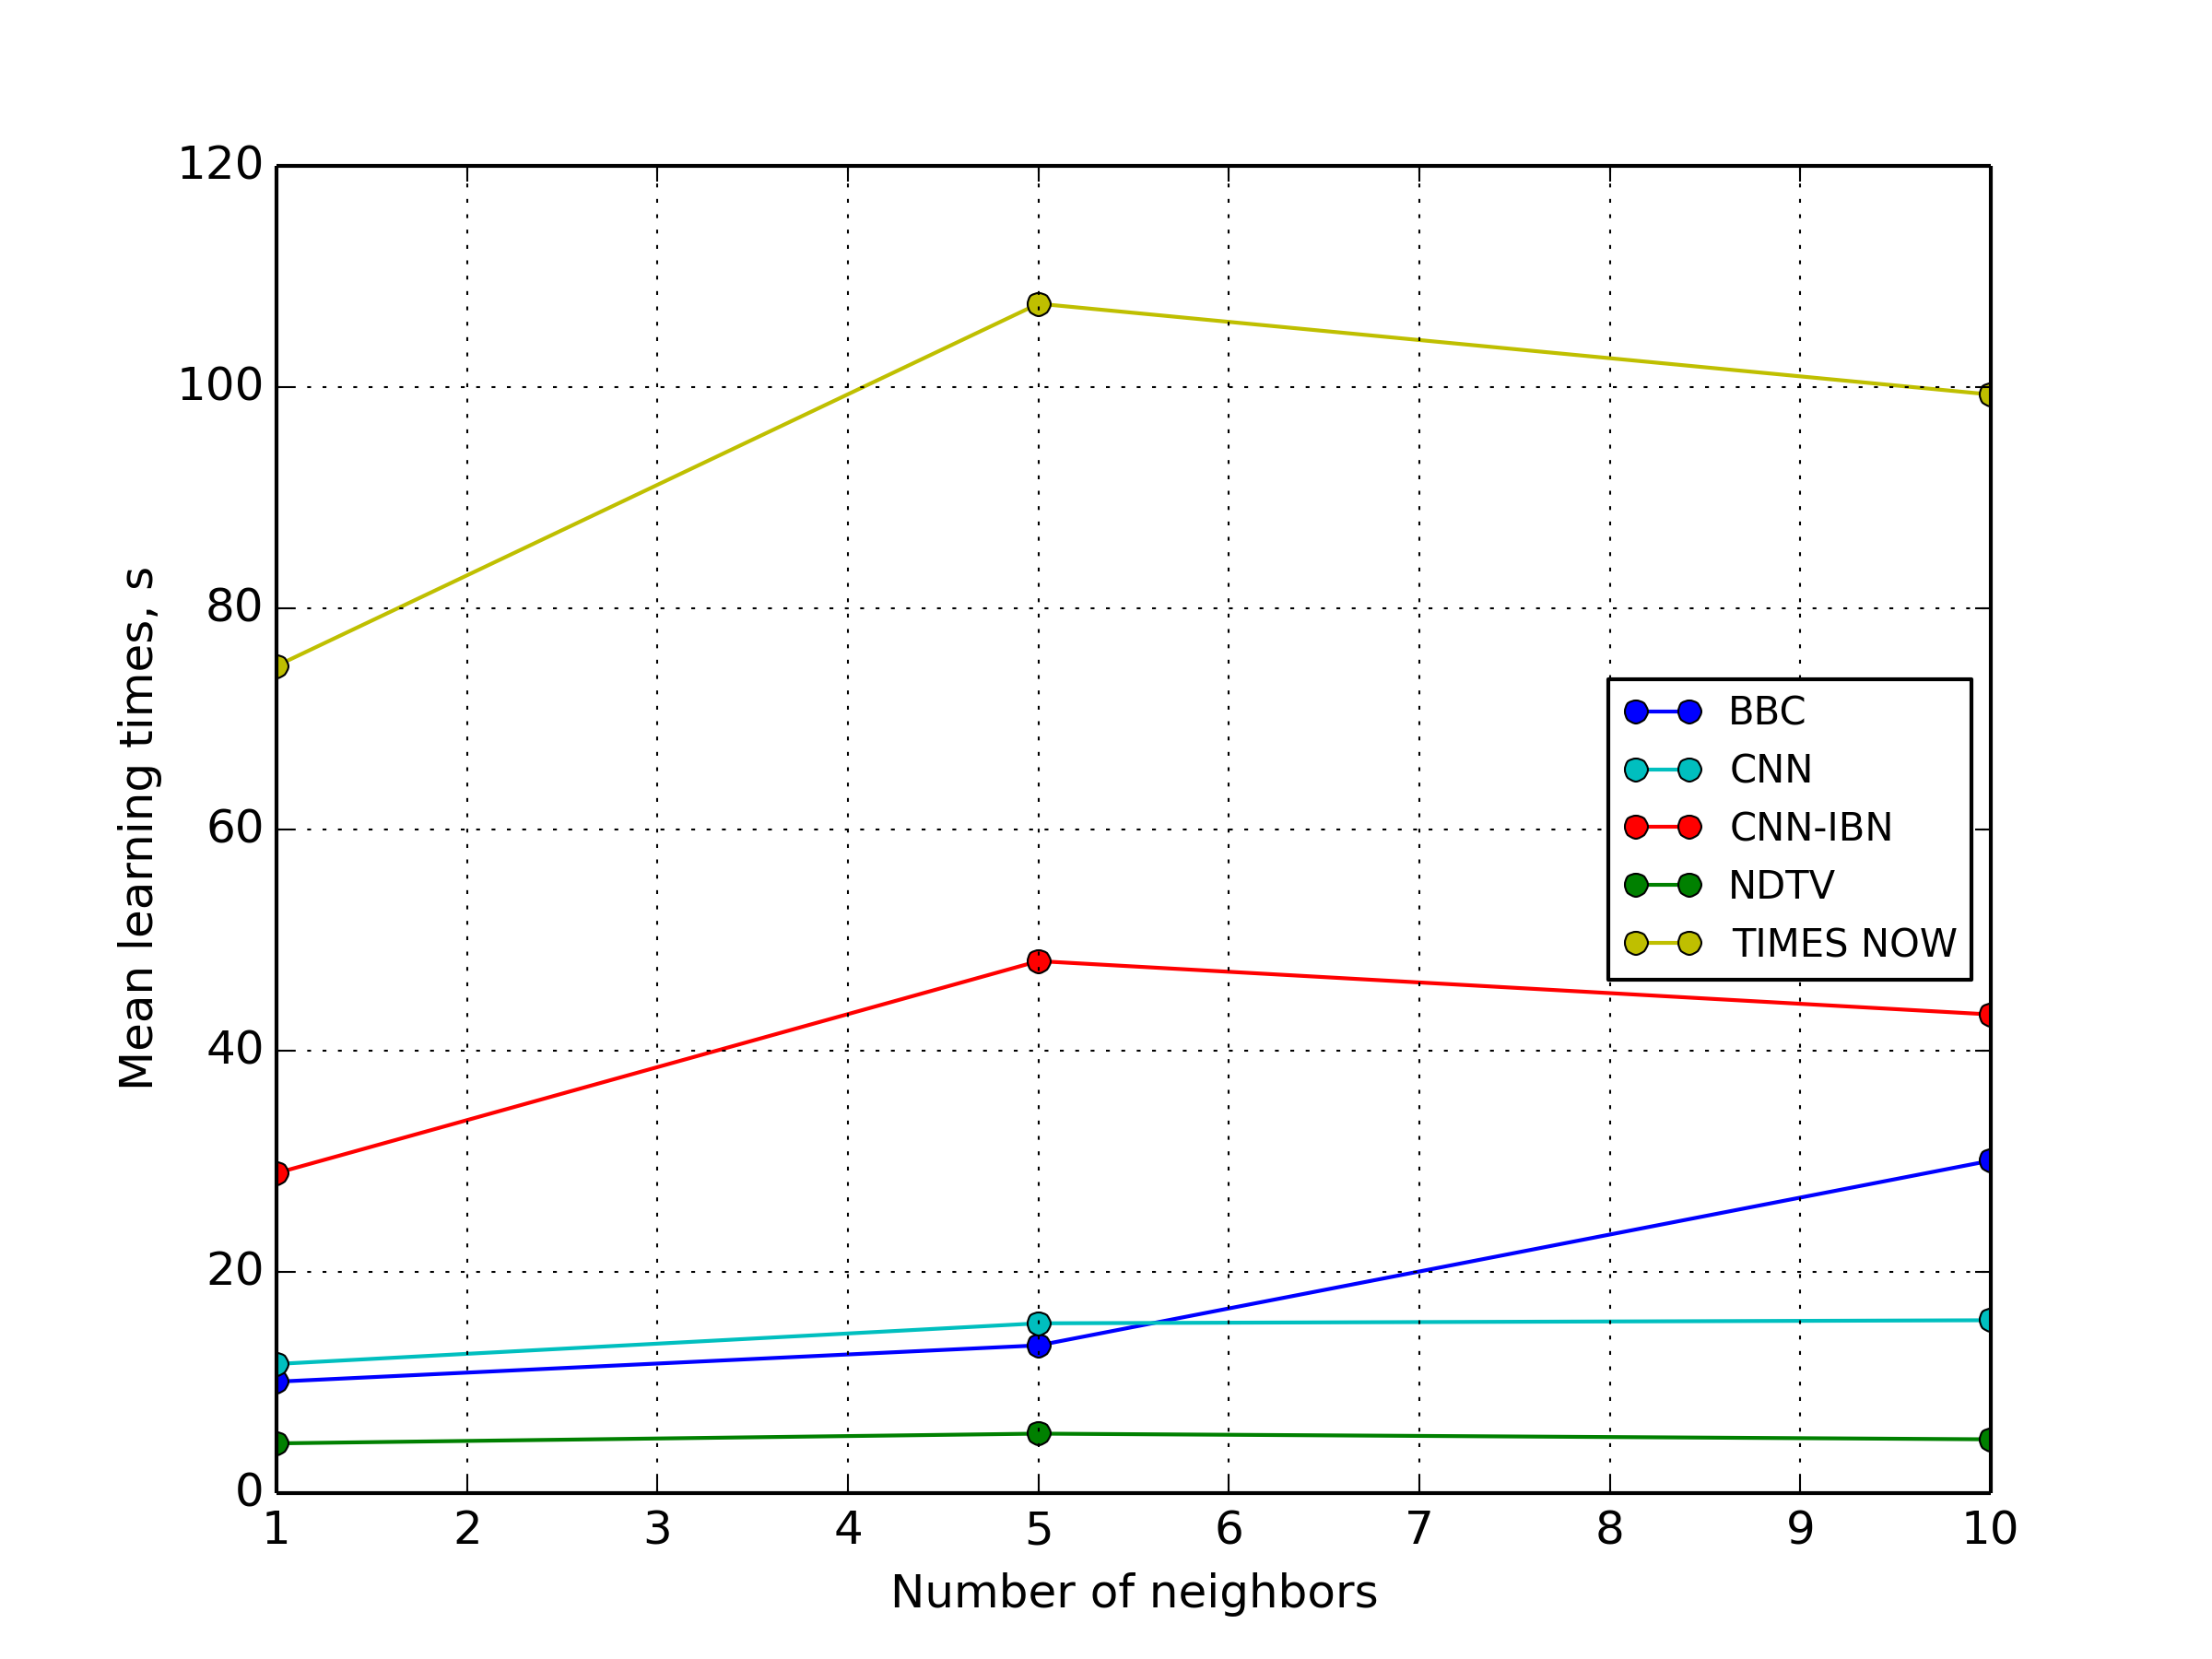
\includegraphics[width=\textwidth]{images/fcnn-SVMTime.png}
		\caption{Время обучения.}
	\end{subfigure}
	\caption{Результаты применения FCNN для SVM.}\label{fig:fcnn-svm-results}
\end{figure}

\begin{figure}[h!]
	\centering
	\begin{subfigure}{0.45\textwidth}
		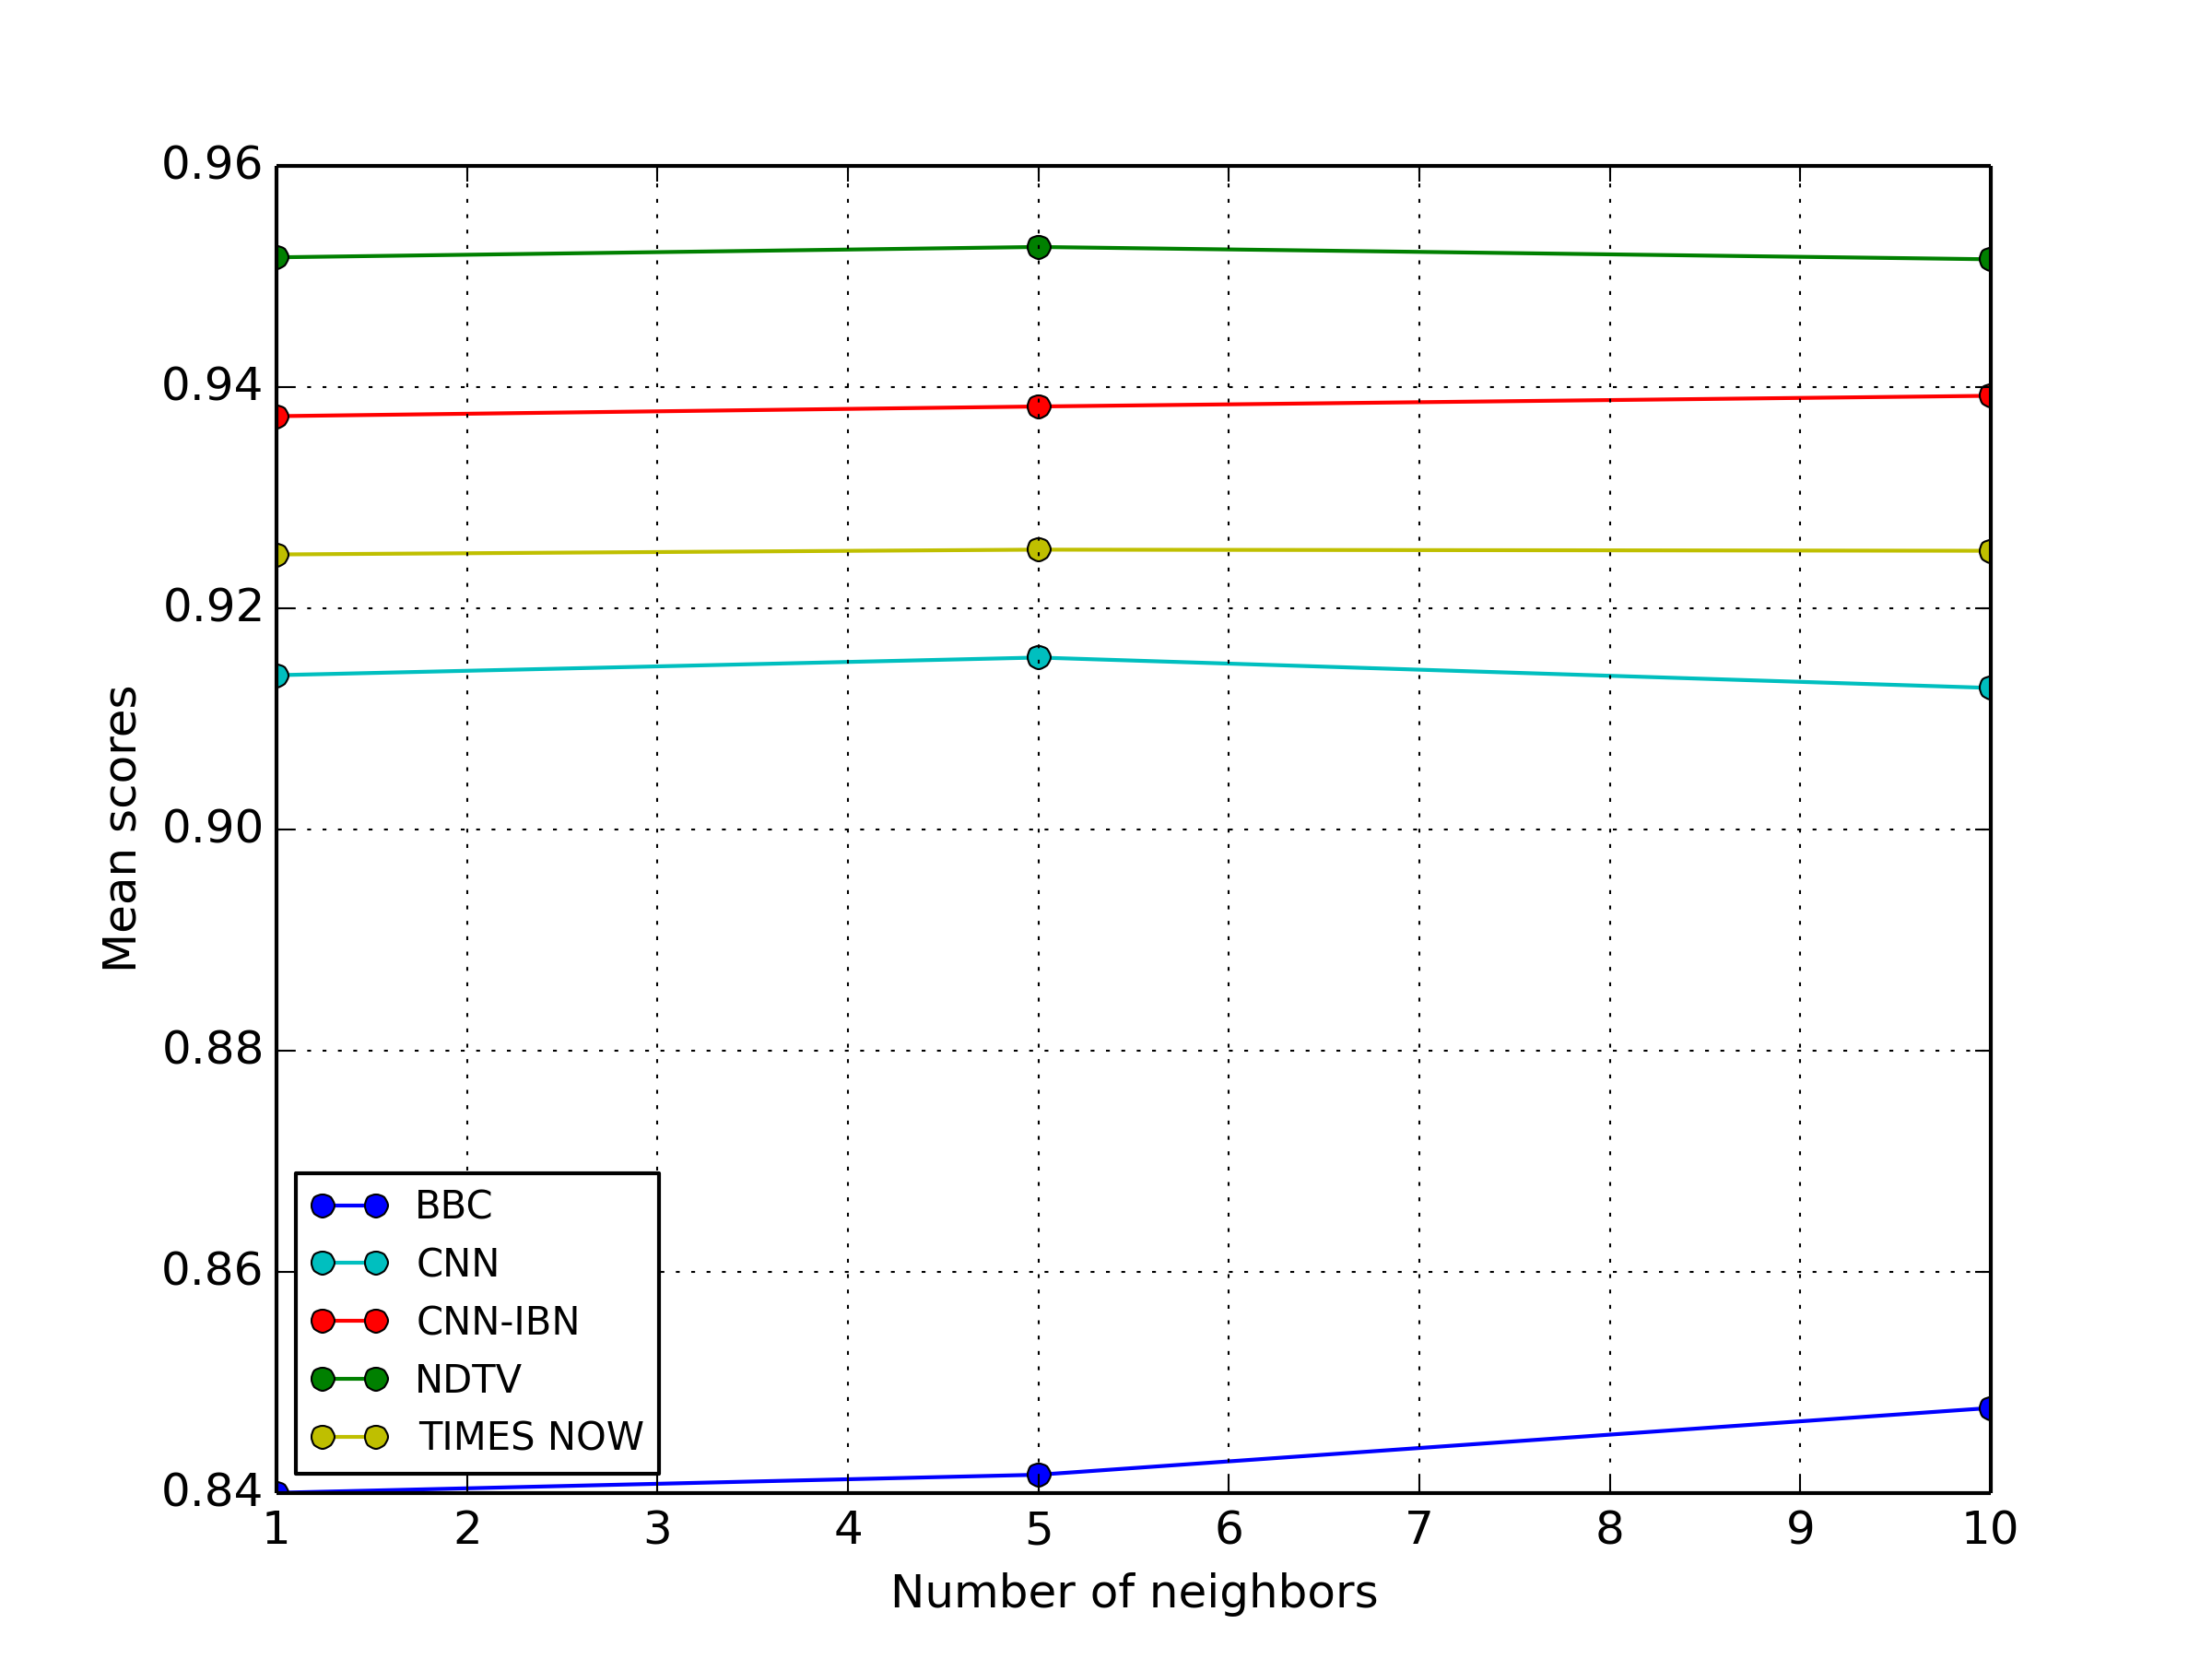
\includegraphics[width=\textwidth]{images/fcnn-randforest.png}
		\caption{Качество классификации.}
	\end{subfigure}
	\begin{subfigure}{0.45\textwidth}
		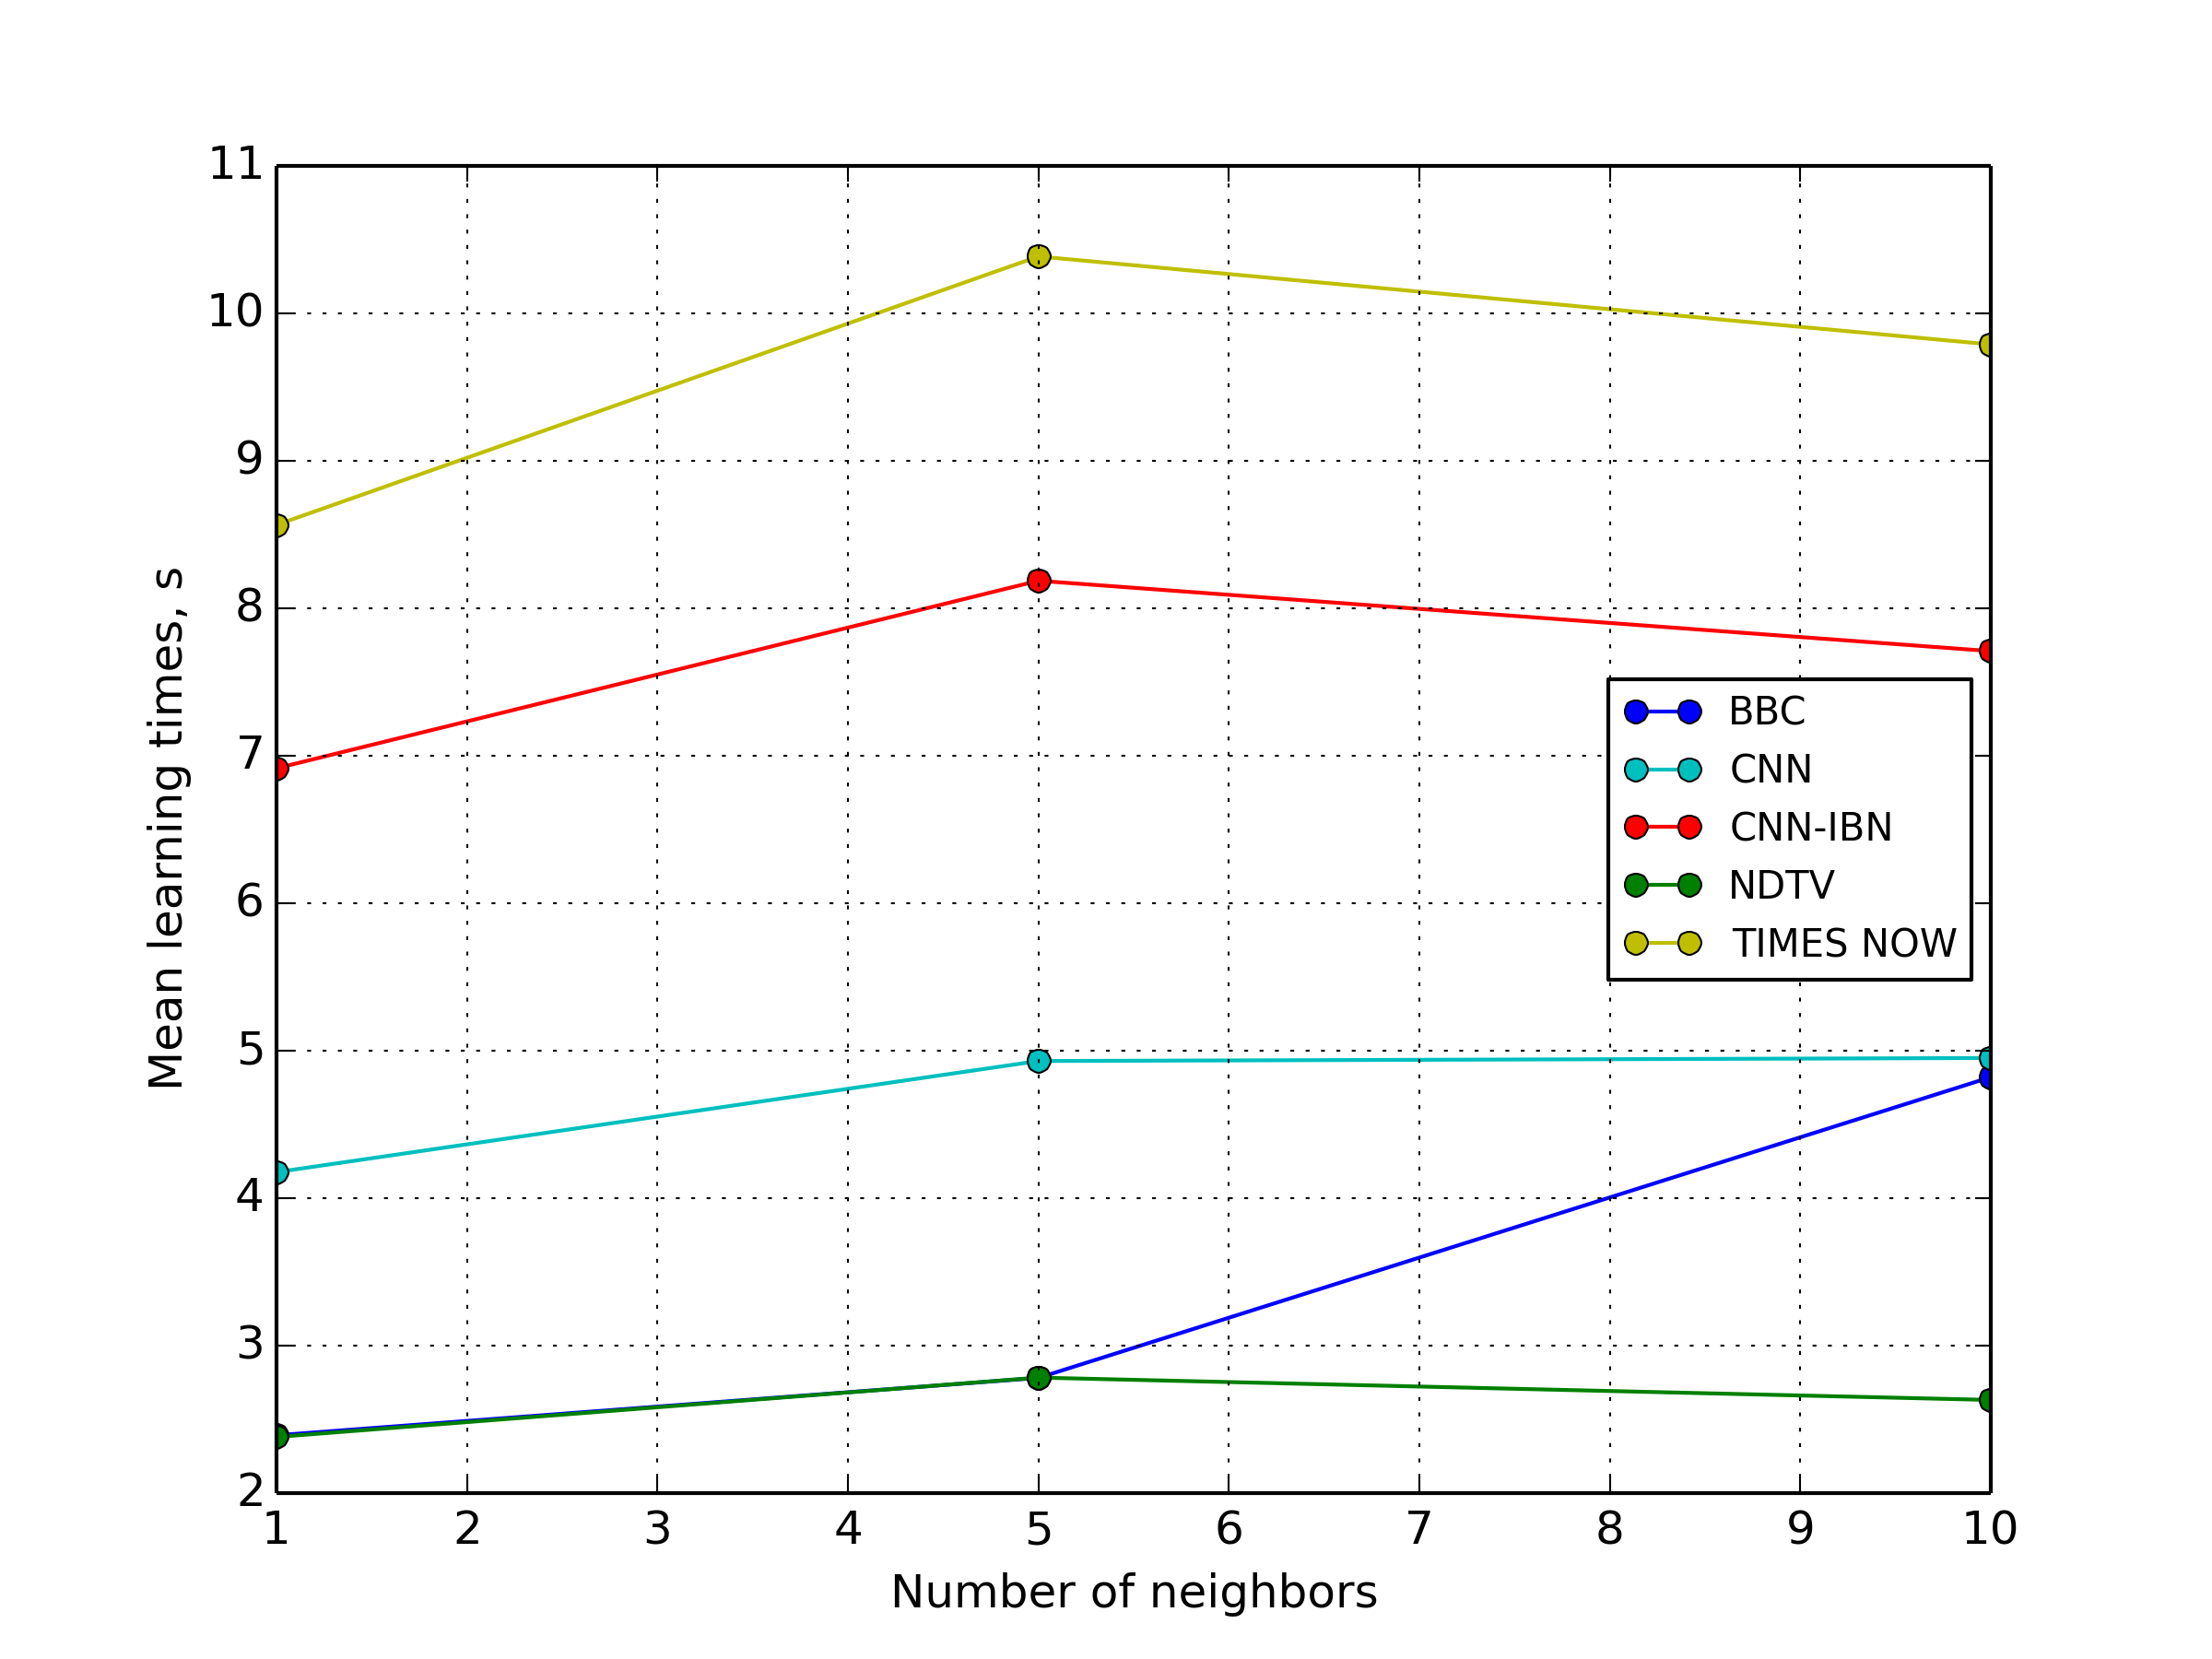
\includegraphics[width=\textwidth]{images/fcnn-randforestTime.png}
		\caption{Время обучения.}
	\end{subfigure}
	\caption{Результаты применения FCNN для Random forest.}\label{fig:fcnn-rf-results}
\end{figure}

\begin{figure}
	\centering
	\begin{subfigure}{0.45\textwidth}
		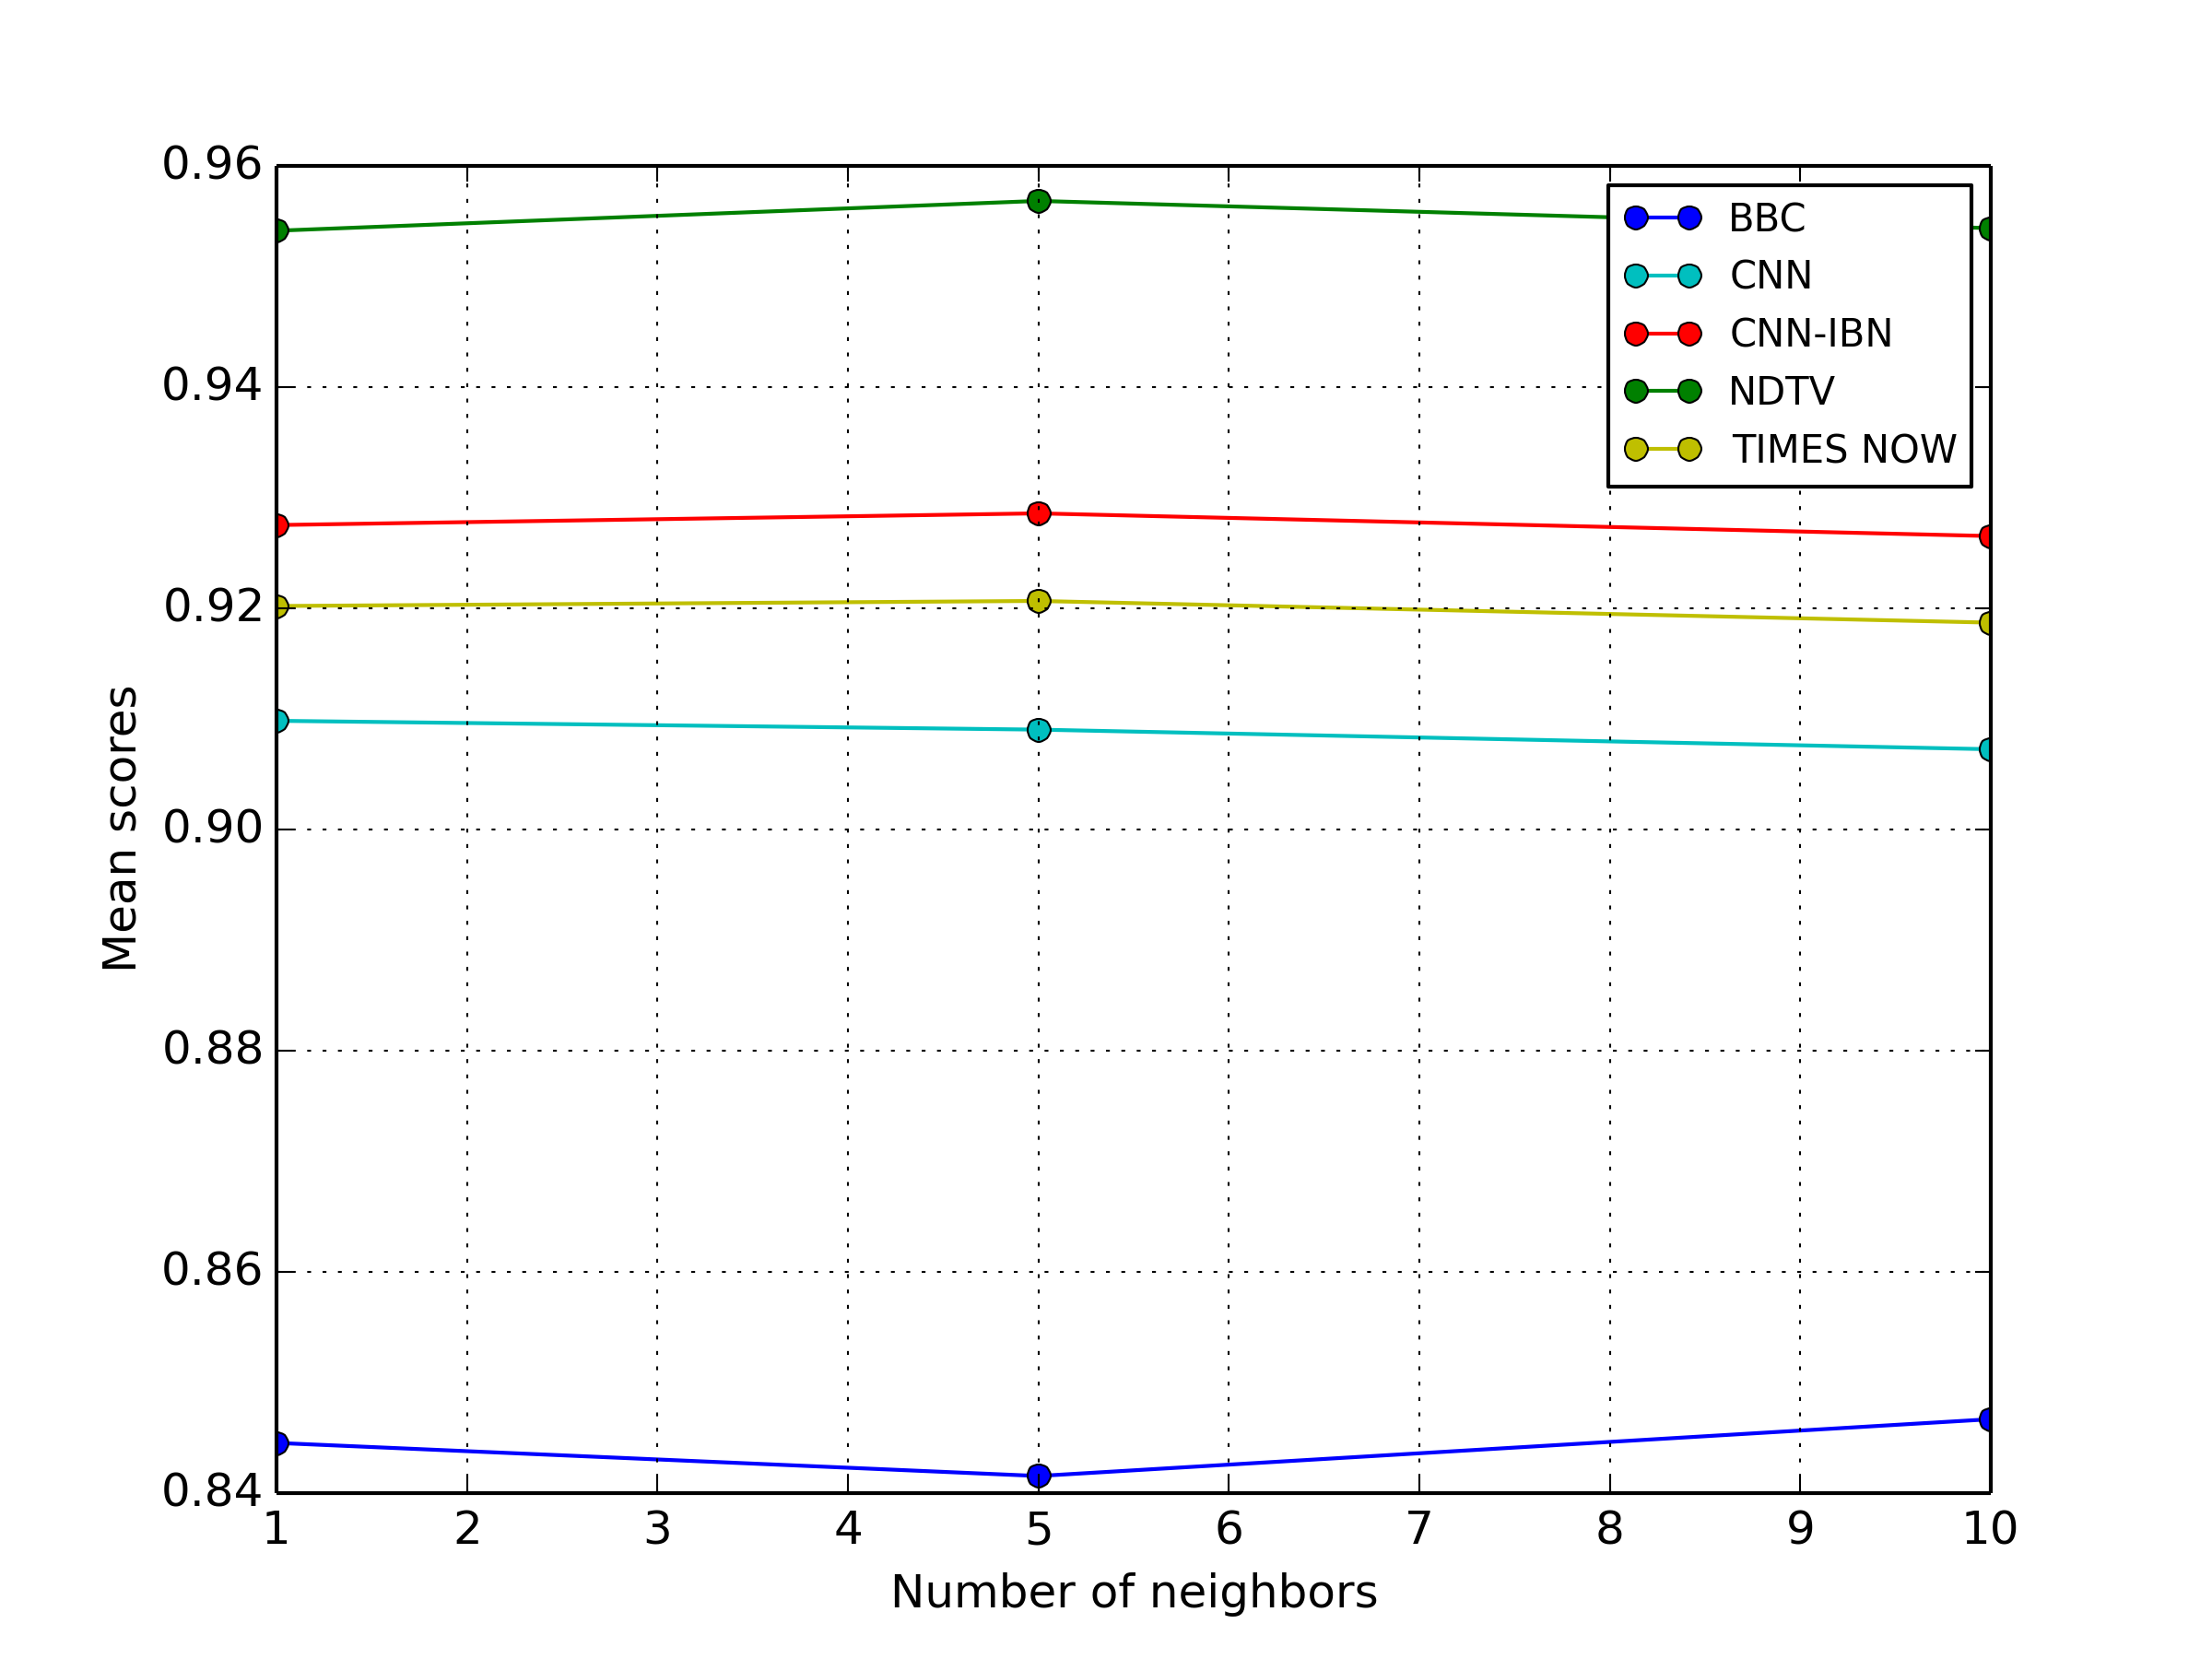
\includegraphics[width=\textwidth]{images/fcnn-gradboosting.png}
		\caption{Качество классификации.}
	\end{subfigure}
	\begin{subfigure}{0.45\textwidth}
		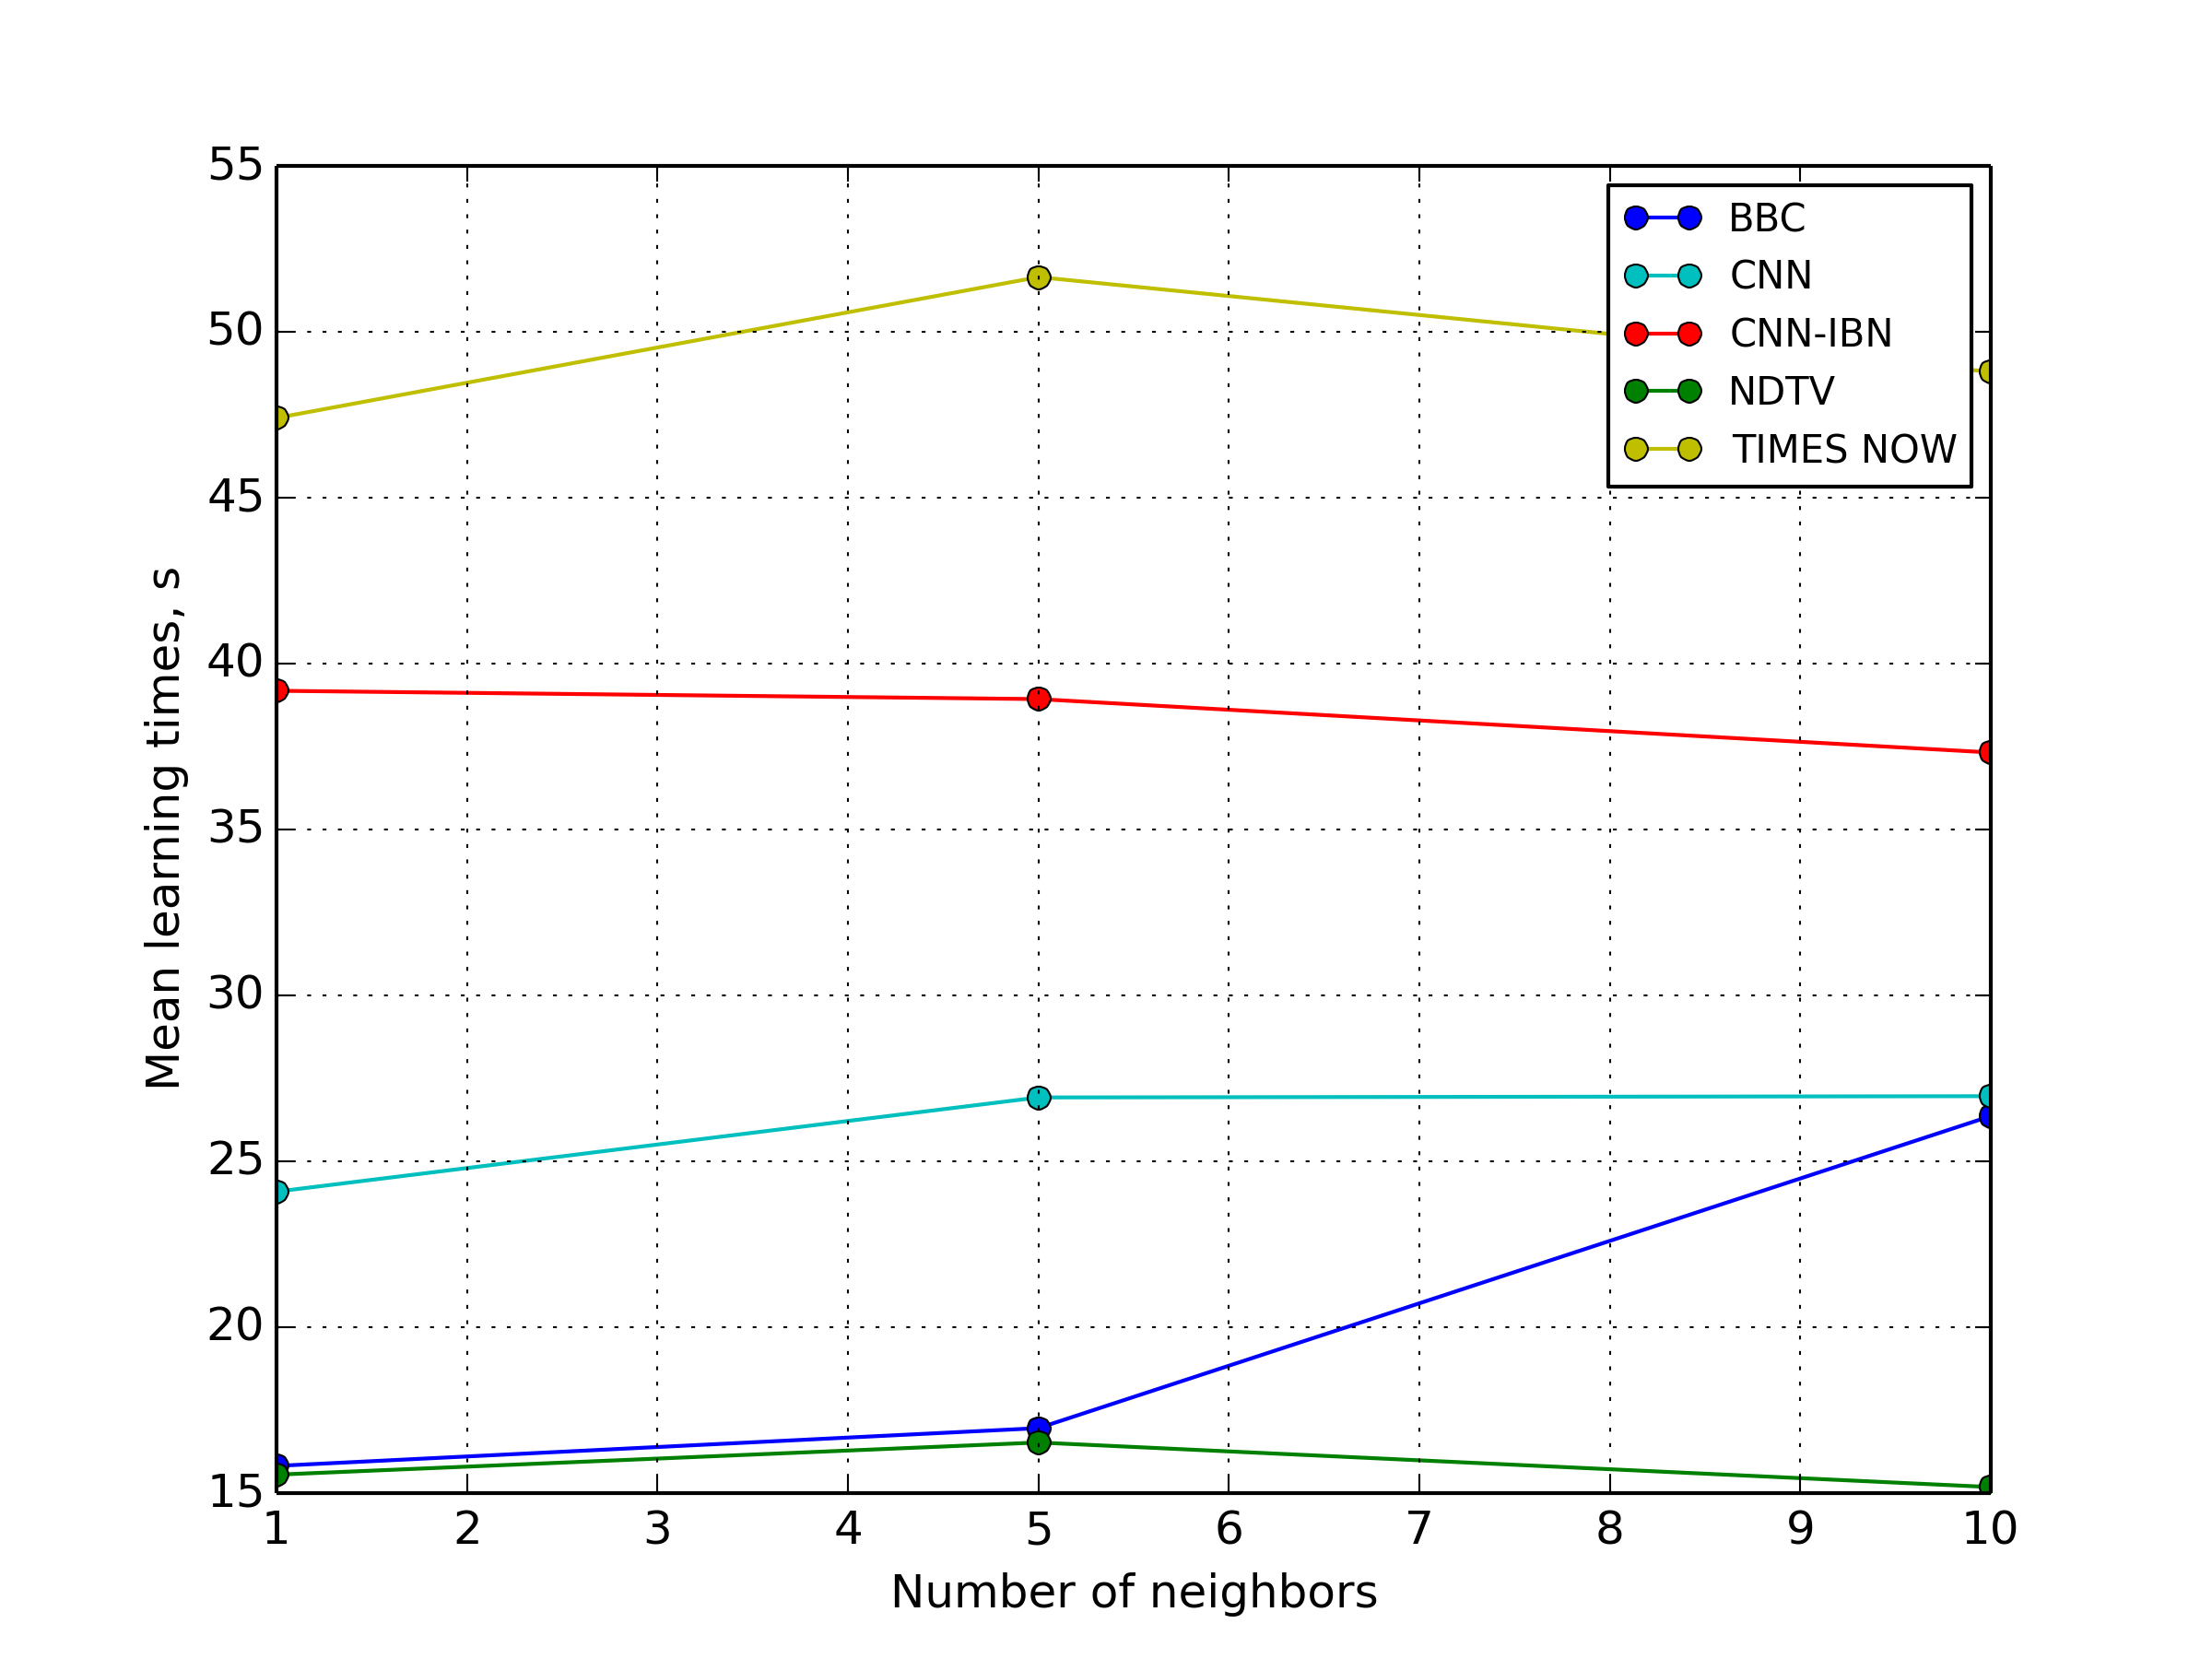
\includegraphics[width=\textwidth]{images/fcnn-gradboostingTime.png}
		\caption{Время обучения.}
	\end{subfigure}
	\caption{Результаты применения FCNN для GTB}\label{fig:fcnn-gtb-results}
\end{figure}

В целом, FCNN генерирует подвыборку немного большую, чем CNN, и тратит на это немного больше времени (в \cite{angiulli} указано, что FCNN имеет лучшую асимптотику, чем CNN, что может быть проверено на ещё больших наборах данных). Но это сполна компенсируется тем, что при сравнимых затратах времени на обучение базовых методов качество классификации оказывается у них намного выше, чем после CNN. FCNN всё равно приводит к ухудшению качества классификации, но по результатам экспериментов для \(k=1\) это ухудшение не превышает 1.9\%. Соответствующие данные приведены в таблице~\ref{table:fcnn-results} с использованием обозначений, аналогичных таблице~\ref{table:cnn-results}.

\begin{table}[h!]
    \centering
    \begin{tabular}{|c||c||c|c|}
    \cline{2-4}
    \multicolumn{1}{c||}{} & Сжатие \(T\) & \(k\)NN & LDA \\
    \hline \hline
	\input{fcnn-table1.txt}
\end{tabular}
\newline \vspace*{0.5cm} \newline
\begin{tabular}{|c||c|c|c|}
    \cline{2-4}
    \multicolumn{1}{c||}{} & SVM & Random forest & GTB \\
    \hline \hline
	\input{fcnn-table2.txt}
    \end{tabular}
    \caption{Сводная таблица результатов метода FCNN и базовых методов после применения FCNN}
    \label{table:fcnn-results}
\end{table}

\subsection{Class conditional instance selection}
CCIS \cite{marchiori} отличается от двух предыдущих методов тем, что он принадлежит к категории гибридных методов отбора эталонов. Он состоит из двух этапов: классово-условный выбор эталонов (CC) и прорежение (THIN).

Центральным для данного метода является граф классово-условных ближайших соседей \(G=(V,E)\) --- орграф, вершинам \(v\in V\) которого соответствуют элементы \(T\), а ребро \((a,b)\in E\), если \(b\) есть ближайший сосед \(a\) для некоторого класса. \(G\) разбивается на 2 подграфа: \(G_{wc}=(V,E_{wc})\), в котором есть лишь те рёбра из \(G\), которые инцидентны двум вершинам одного класса и \(G_{bc}=(V,E_{bc})\), в котором есть лишь те рёбра из \(G\), которые инцидентны двум вершинам разных классов. Полустепень захода в первом называется внутриклассовой полустепенью захода (within class in-degree), во втором --- междуклассовой полустепенью захода (between class in-degree).

Классово-условный отбор эталонов составляет подмножество \(S\) обучающей выборки \(T\), добавляя в него элементы по одному пока Leave-one-out-ошибка, полученная методом ближайшего соседа на \(S\), убывает и больше LOO-ошибки, полученной на \(T\). Порядок, в котором элементы \(T\) выбираются для добавления в \(S\), обусловлен теоретико-информационным критерием, зависящим от полустепеней захода элемента в \(G_{wc}\) и \(G_{bc}\), и характеризующим то, насколько глубоко объект находится внутри своего класса. В частности, из \(T\) удалятся все объекты, для которых междуклассовая полустепень захода больше внутриклассовой (такие элементы, скорее всего, лежат близко к границе классов.

Прорежение призвано отфильтровать \(S\), оставив объекты, наиболее важные для определения границы классов. Для этого из \(S\) выбирается подмножество \(S_f\), состоящее из объектов с положительной междуклассовой полустепенью захода в графе \(G^S\) для выборки \(S\) (эти объекты считаются важными для определения границы между классами). Затем \(S_f\) дополняется объектами из \(S\setminus S_f\) пока LOO-ошибка на \(T\) при использовании \(S_f\) в качестве обучающей выборки уменьшается.

\subsubsection*{Результаты использования CCIS}
Идея графа классово-условных ближайших соседей ориентирована на использование с методом одного ближайшего соседа, поэтому CCIS не имеет параметров. Таблица~\ref{table:ccis-results} содержит результаты работы CCIS и базовых методов после отбора им эталонов. В плюсы CCIS можно записать отличную редукцию обучающей выборки --- результат CCIS в нашей задаче имеет не более 10\% элементов исходной обучающей выборки, и, как следствие, большое ускорение тех базовых методов, которые изначально имели сколько-нибудь значительное время работы. \(k\)NN, случайный лес и градиентный бустинг ускорились более, чем в 10 раз, а SVM --- более, чем в 100, на всех каналах. Несомненным минусом CCIS является тот факт, что в нашей задаче он не смог обеспечить не только повышение качества классификации, но и удержание его на уровне данных из таблицы~\ref{table:base-all}. Данный результат приводит к мысли о том, что CCIS может быть полезен разве что для редукции сверхбольших выборок, с которыми невозможно работать в их полном составе. Хотя и в этом случае, скорее всего, есть более подходящие методы.

\begin{table}[h!]
    \centering
    \begin{tabular}{|c||c||c|c|}
    \cline{2-4}
    \multicolumn{1}{c||}{} & Сжатие \(T\) & \(k\)NN & LDA \\
    \hline \hline
	\input{ccis-table1.txt}
\end{tabular}
\newline \vspace*{0.5cm} \newline
\begin{tabular}{|c||c|c|c|}
    \cline{2-4}
    \multicolumn{1}{c||}{} & SVM & Random forest & GTB \\
    \hline \hline
	\input{ccis-table2.txt}
    \end{tabular}
    \caption{Сводная таблица результатов метода CCIS и базовых методов после применения CCIS}
    \label{table:ccis-results}
\end{table}

